
%%==================================================
%% demo.tex for BIT Thesis
%% modified by yang yating
%% version: 1.2
%% last update: Jan. 4th, 2018
%%==================================================


\documentclass[cn,11pt,fancy,hide,pad]{config}


\title{语音识别学习笔记}
\subtitle{学习大法好}

\author{杜沪}
\institute{BIT, SpeechOcean}
\date{\today}
\version{0.1}

\equote{Victory won\rq t come to us unless we go to it. --- M. Moore}

\logo{logo.png}
\cover{cover.jpg}



\begin{document}
\maketitle
\tableofcontents
\listoffigures
\listoftables

% \thispagestyle{empty}

\mainmatter
\hypersetup{pageanchor=true}

%% 各章正文内容
%\section{HMM相关知识点总结}
\subsection{basic infomation}
设Q是所有可能状态的集合,V是所有可能观测的集合。其中$N$是可能的状态数,$M$是可能的观测数。
\begin{center}
$Q=\{q_1, q_2, ..., q_N\}$, $V = \{v_1, v_2, ..., v_M\}$
\end{center}

$I$是长度为$T$的状态序列,$O$是对应的观测序列。
\begin{center}
$I=\{i_1, i_2, ..., i_T\}$, $O = \{o_1, o_2, ..., o_T\}$
\end{center}

$A$为状态转移矩阵,如公式\ref{trans-matrix},其中$a_{ij}=P(i_{t+1}=q_j|i_t=q_i)$,$i=1,2,...,N; j=1,2,...,N$,是在时刻$t$处于状态$q_i$的条件下在时刻$t+1$转移到状态$q_j$的概率。
\begin{align}
\label{trans-matrix}
A=[a_{ij}]_{N\times{N}}
\end{align}

$B$是观测概率矩阵,如公式\ref{emit-matrix},其中$b_j(k)=P(o_t=v_k|i_t=q_j)$,$k=1,2,...,M; j=1,2,...,N$是$t$时刻处于状态$q_j$的条件下生成观测$v_k$的概率。
\begin{align}
\label{emit-matrix}
B=[b_{j}(k)]_{N\times{M}}
\end{align}

$\pi$是初始状态概率向量,如公式\ref{init-vector},其中$\pi_i=P(i_1=q_i)$,$i=1,2,...,N$。
\begin{align}
\label{init-vector}
\pi = (\pi_i)
\end{align}

HMM有三个基本问题:

(1)概率计算问题。给定模型$\lambda=(A,B,\pi)$和观测序列$O=(o_1, o_2, ..., o_T)$,计算在模型$\lambda$的条件下观测序列$O$出现的概率$P(O|\lambda)$。

(2)学习问题。已知观测序列$O=(o_1, o_2, ..., o_T)$,估计模型$\lambda=(A,B,\pi)$参数,使得在该模型下观测序列$P(O|\lambda)$最大,即用最大似然估计的方法估计参数。

(3)预测问题,也称为解码问题。已知模型$\lambda=(A,B,\pi)$和观测序列$O=(o_1, o_2, ..., o_T)$,求对给定观测序列条件概率$P(I|O)$最大的状态序列$I=\{i_1, i_2, ..., i_T\}$,即给定观测序列,求最有可能的对应的状态序列。

\subsection{概率计算问题}
\subsubsection{前向算法}

\subsubsection{后向算法}

\subsection{学习问题}

\subsection{解码问题}
\chapter{数学知识总结}

%------------------------------------------------------------------------------
%                                Matrix Definations
%------------------------------------------------------------------------------
\section{各类矩阵定义}
%转置矩阵
\begin{definition}{\hypertarget{transpose}{转置矩阵}}{int}
\label{def:transpose}
把矩阵$A$的行换乘同序数的列得到一个新矩阵,就叫做$A$的转置矩阵,记作$A^{T}$。例如矩阵
\begin{align}
A = 
\begin{bmatrix}
1 & 2 & 0 \\
3 & -1 & 1
\end{bmatrix}
\end{align}
的转置矩阵为
\begin{align}
A^{T} = 
\begin{bmatrix}
1 & 3 \\
2 & -1 \\
0 & 1
\end{bmatrix}
\end{align}
\end{definition}

%对称矩阵
\begin{definition}{\hypertarget{symmetric}{对称矩阵}}{int}
\label{def:symmetric}
设$A$为$n$阶方阵,如果满足$A^T=A$,即:
\begin{align}
a_{ij} = a_{ji}  (i,j=1, 2, ..., n)
\end{align}
那么$A$称为对称矩阵,简称为对称阵。对称阵的特点是:它的元素以对角线为对称轴对应相等。
\end{definition}

%复共轭矩阵
\begin{definition}{\hypertarget{ctranspose}{复共轭矩阵}}{int}
\label{def:ctranspose}
设$A\in{C^{m\times{n}}}$,用$\bar{A}$表示以$A$的元素的共轭复数为元素组成的矩阵,命:
\begin{align}
A^{H} = (\bar{A})^{T}
\end{align}
则称$A^{H}$为$A$的复共轭转置矩阵。
\end{definition}

%Hermitian矩阵
\begin{definition}{\hypertarget{hermitian}{Hermitian矩阵}}{int}
\label{def:hermitian}
设$A\in{R^{n\times{n}}}$,若$A^{H}=A$,则称$A$为Hermitian矩阵。若$A^{H}=-A$,则称$A$为反Hermitian矩阵。
\end{definition}

%正交矩阵
\begin{definition}{\hypertarget{orthogonal}{正交矩阵}}{int}
\label{def:orthogonal}
如果$n$阶矩阵$A$满足
\begin{align}
A^{T}A=E
\end{align}
即:
\begin{align}
A^{T}=A^{-1}
\end{align}
则称$A$为正交矩阵,简称正交阵。
\end{definition}

%酉矩阵
\begin{definition}{\hypertarget{unitary}{酉矩阵}}{int}
\label{def:unitary}
如果$n$阶复矩阵$A$满足
\begin{align}
A^{H}A=AA^{H}=E
\end{align}
则称$A$为酉矩阵,记作$A\in{U^{n\times{n}}}$。
\end{definition}

%奇异矩阵
\begin{definition}{\hypertarget{singular}{奇异矩阵}}{int}
\label{def:singular}
当$|A|=0$时,$A$称为奇异矩阵,否则称为非奇异矩阵。$A$是可逆矩阵的充分必要条件是$|A|\neq{0}$,即可逆矩阵就是非奇异矩阵。
\end{definition}

%正规矩阵
\begin{definition}{\hypertarget{formal}{正规矩阵}}{int}
\label{def:formal}
设$A\in{C^{n\times{n}}}$,若:
\begin{align}
A^{H}A=AA^{H}
\end{align}
则称$A$为正规矩阵,$A\in{R^{n\times{n}}}$,显然有$A^{H}=A^{T}$,上式就变成了:
\begin{align}
A^{T}A=AA^{T}
\end{align}
则称$A$为实正规矩阵。
\end{definition}

%幂等矩阵
\begin{definition}{\hypertarget{power}{幂等矩阵}}{int}
\label{def:power}
设$A\in{C^{n\times{n}}}$,若:
\begin{align}
A^{2}=A
\end{align}
则称$A$是幂等矩阵。
\end{definition}

%正定矩阵
\begin{definition}{\hypertarget{positive}{正定矩阵}}{int}
\label{def:positive}
设$A\in{C^{n\times{n}}}$,若A的所有特征值均为正数,则称$A$为正定矩阵;若$A$的特征值均为非负数,则称$A$为版正定矩阵。

判断一个矩阵为正定矩阵的充要条件有:
\begin{enumerate}
\item $A$的所有特征值$\lambda_{i}$均为正数;
\item $x^{T}Ax \ge 0$对所有非零向量$x$都成立;
\item 存在秩满矩阵$R$,使得$A=R^{T}R$。
\end{enumerate}
\end{definition}

%Jacobi矩阵
\begin{definition}{\hypertarget{power}{Jacobi矩阵}}{int}
\label{def:jacobi}
假设某函数从$f:R^{n}\rightarrow R^{m}$,从$x\in{R^{n}}$映射到向量$f(x)\in{R^{m}}$,其Jacobi矩阵的维度是$m\times{n}$,如下所示:
\begin{align}
H = 
\begin{bmatrix}
\frac{\partial f}{\partial x_{1}} & \frac{\partial f}{\partial x_{1}} & \cdots & \frac{\partial f}{\partial x_{n}} 
\end{bmatrix}
 =
\begin{bmatrix}
\frac{\partial f_{1}}{\partial x_{1}}  & \frac{\partial f_{1}}{\partial x_{2}} & \cdots & \frac{\partial f_{1}}{\partial x_{n}} \\
\frac{\partial f_{2}}{\partial x_{1}}  & \frac{\partial f_{2}}{\partial x_{2}} & \cdots & \frac{\partial f_{2}}{\partial x_{n}} \\
\vdots        & \vdots        & \ddots    & \vdots \\
\frac{\partial f_{m}}{\partial x_{1}}  & \frac{\partial f_{m}}{\partial x_{2}} & \cdots & \frac{\partial f_{m}}{\partial x_{n}} \\
\end{bmatrix}
\end{align}
\end{definition}

%Hessian矩阵
\begin{definition}{\hypertarget{power}{Hessian矩阵}}{int}
\label{def:hessian}
若实值函数$f(x_1, x_2, ..., x_n)$的所有二阶偏导都存在并在定义域内连续,那么函数$f$的Hessian矩阵为:
\begin{align}
H = 
\begin{bmatrix}
\frac{\partial^{2}f}{\partial x_{1}^{2}}  & \frac{\partial^{2}f}{\partial x_{1}x_{2}} & \cdots & \frac{\partial^{2}f}{\partial x_{1}x_{n}} \\
\frac{\partial^{2}f}{\partial x_{2}x_{1}} & \frac{\partial^{2}f}{\partial x_{2}^{2}}  & \cdots & \frac{\partial^{2}f}{\partial x_{2}x_{n}} \\
\vdots        & \vdots        & \ddots    & \vdots \\
\frac{\partial^{2}f}{\partial x_{n}x_{1}} & \frac{\partial^{2}f}{\partial x_{n}x_{2}} & \cdots & \frac{\partial^{2}f}{\partial x_{n}^{2}} \\
\end{bmatrix}
\end{align}
根据:
\begin{align}
\frac{\partial^{2}f}{\partial x_{1}x_{2}}  = \frac{\partial^{2}f}{\partial x_{2}x_{1}} 
\end{align}
可知Hessian矩阵为对称阵。
\end{definition}
%------------------------------------------------------------------------------
%                                         瑞利商
%------------------------------------------------------------------------------
\section{瑞利商}
\label{sec:rayleigh-quotient}
对于一个\hyperlink{hermitian}{Hermitian矩阵}$M$及非零向量$x$,\href{https://en.wikipedia.org/wiki/Rayleigh_quotient}{瑞利商}(Rayleigh quotient)的定义如公式\ref{eqn:ray1},其中$x^{H}$为$x$的共轭转置向量。
\begin{align}
\label{eqn:ray1}
R(M,x)=\frac{x^{H}Mx}{x^{H}x}
\end{align}

若$M$和$x$中元素均为实数,瑞利商可以写成公式\ref{eqn:ray2}。
\begin{align}
\label{eqn:ray2}
R(M,x)=\frac{x^{T}Mx}{x^{T}x}
\end{align}

设M的特征值与特征向量分别为$\lambda_1, ..., \lambda_n$和$v_1, .., v_n$,且满足 $\lambda_{\min}=\lambda_1\leq{\lambda_2}\leq{...}\leq{\lambda_n}=\lambda_{\max}$,那么在M已知的情况下有:
\begin{align}
\label{eqn:conc-ray}
\begin{split}
cR(M,x) &= \lambda_{n} \\
\mathop{\min}_{x}R(M,x) &= \lambda_{1}
\end{split}
\end{align}

以下为证明公式\ref{eqn:conc-ray}的过程:

由于$M$是Hermitian矩阵,存在一个酉矩阵$U$,满足公式\ref{eqn:unity-matrix}。
\begin{align}
\label{eqn:unity-matrix}
M=UAU^{T}
\end{align}
其中$A=diag\{\lambda_1, ..., \lambda_n\}$。

因此公式\ref{eqn:ray2}可以转换如下:
\begin{align}
\begin{split}
R(M,x) &= \frac{x^{T}UAU^{T}x}{x^{T}x} \\
       &= \frac{(U^{T}x)^{T}A(U^{T}x)}{x^{T}x}  
\end{split}
\end{align}

设$P=U^{T}x$,则:
\begin{align}
\label{eqn:trans1}
\begin{split}
R(M,x) &= \frac{P^{T}AP}{x^{T}x} \\
       &= \frac{\sum_{i=1}^{n}\lambda_{i}|P_i|^{2}}{\sum_{i=1}^{n}|x_i|^{2}}
\end{split}
\end{align}

根据特征值的大小关系,我们可以得到不等式\ref{eqn:feature-unequal}。
\begin{align}
\label{eqn:feature-unequal}
\lambda_{1}\sum_{i=1}^{n}|P_i|^{2} \leq \sum_{i=1}^{n}\lambda_{i}|P_i|^{2} \leq \lambda_{n}\sum_{i=1}^{n}|P_i|^{2}
\end{align}

所以公式\ref{eqn:trans1}的范围如下:
\begin{align}
\label{eqn:trans0}
\lambda_{1}\frac{\sum_{i=1}^{n}|P_i|^{2}}{\sum_{i=1}^{n}|x_i|^{2}} \leq R(M,x) \leq \lambda_{n}\frac{\sum_{i=1}^{n}|P_i|^{2}}{\sum_{i=1}^{n}|x_i|^{2}} 
\end{align}

设$U$第$i$行第$j$列的元素为$u_{ij}$,则$U^{T}$第$i$行第$j$列的元素为$u_{ji}$,由$P=U^{T}x$和$P^{T}=x^{T}U$可得:
\begin{align}
\begin{split}
p_i &= \sum_{i=1}^{n} u_{ji}x_j \\
p_{i}^{T} &= \sum_{j=1}^{n} x_{i}u_{ij}
\end{split}
\end{align}

则:

\begin{align}
|p_i|^{2} = p_{i}^{T}p_i = \sum_{j=1}^{n} \sum_{k=1}^{n} x_j u_{ij} u_{ki} x_k
\end{align}

于是:
\begin{align}
\label{eqn:trans2}
\begin{split}
\sum_{i=1}^{n}|p_i|^{2} &= \sum_{i=1}^{n} p_{i}^{T}p_i \\
                        &= \sum_{i=1}^{n} \sum_{j=1}^{n} \sum_{k=1}^{n} x_j u_{ij} u_{ki} x_k \\
                        &= \sum_{j=1}^{n} \sum_{k=1}^{n} (\sum_{i=1}^{n} u_{ki} u_{ij}) x_j x_k 
\end{split}
\end{align}

因为$U$是酉矩阵,满足$U^{T}U=I$,所以:
\begin{align}
I_{jk} = \sum_{i=1}^{n} u_{ji} u_{ik}
\end{align}

其满足如下等式:
\begin{equation}
\label{eqn:trans3}
I_{jk}=\left\{
\begin{array}{rcl}
1 & & j = k\\
0 & & j \neq k
\end{array} \right
\end{equation}

结合\ref{eqn:trans2}和\ref{eqn:trans3}可得如下等式:
\begin{align}
\sum_{i=1}^{n}|p_i|^{2} = \sum_{i=1}^{n} |x_i|^2
\end{align}

代入公式\ref{eqn:trans0}可得:
\begin{align}
\label{eqn:trans4}
\lambda_{1} \leq R(M,x) \leq \lambda_{n} 
\end{align}
且:
\begin{equation}
\label{eqn:trans5}
R(M,x)=\left\{
\begin{array}{rcl}
\lambda_{1} & & x = v_1\\
\lambda_{n} & & x = v_n
\end{array} \right
\end{equation}

如果用$x^{'}=cx$代入公式\ref{eqn:ray2}有:
\begin{align}
\begin{split}
R(M,x^{'})  &=\frac{x^{'}^{T}Mx^{'}}{x^{'}^{T}x^{'}}  \\
            &=\frac{c^{2}x^{T}Mx}{c^{2}x^{T}x}  \\
            &=\frac{x^{T}Mx}{x^{T}x} 
\end{split}
\end{align}

由此可以看出来对$x$进行缩放不影响瑞利商的值,即:
\begin{align}
R(M,cx) = R(M,x) 
\end{align}

因此我们可以限定$x^Tx=1$,那么公式\ref{eqn:ray2}可以简化为:
\begin{align}
R(M,x) = x^{T}Mx
\end{align}

那么$R(M,x)$的极值就可以转换成约束条件下的拉格朗日乘法,如公式\ref{eqn:lage}。
\begin{align}
\label{eqn:lage}
L(x, \lambda) = x^{T}Mx - \lambda(x^{T}x-1)
\end{align}

对$x$求导并置为0可得:
\begin{align}
\nabla{L(x, \lambda)} = Mx - \lambda{x} = 0
\end{align}
即$M$的特征值能使得瑞利商取极值,且有:
\begin{align}
R(M,x) = \lambda
\end{align}

瑞利商可以推广至广义瑞利商(Generalized Rayleigh Quotient),其形式如公式\ref{eqn:GRQ}。
\begin{align}
\label{eqn:GRQ}
R(A,B,x) = \frac{x^{H}Ax}{x^{H}Bx}
\end{align}
其中$A$, $B$均为$n\times{n}$的Hermitian矩阵,且$B$为正定矩阵。

令$x=B^{-\frac{1}{2}}x^{'}$,广义瑞利商可以改写成:
\begin{align}
\label{eqn:GRQ}
\begin{split}
R(A,B,x) &= \frac{(B^{-\frac{1}{2}}x^{'})^{H}A(B^{-\frac{1}{2}}x^{'}))}{(B^{-\frac{1}{2}}x^{'})^{H}B(B^{-\frac{1}{2}}x^{'})} \\
         &= \frac{x^{'}^{H}(B^{-\frac{1}{2}})^{H}AB^{-\frac{1}{2}}x^{'}}{x^{'}^{H}(B^{-\frac{1}{2}})^{H}BB^{-\frac{1}{2}}x^{'}}  \\
         &= \frac{x^{'}^{H}(B^{-\frac{1}{2}})^{H}AB^{-\frac{1}{2}}x^{'}}{x^{'}^{H}x^{'}}
\end{split}
\end{align}

此时$R(A,B,x)$的最大特征值和最小特征值即为$(B^{-\frac{1}{2}})^{H}AB^{-\frac{1}{2}}$的最大和最小特征值。其实等价于当$M=(B^{-\frac{1}{2}})^{H}AB^{-\frac{1}{2}}$时的$R(M,x^{'})$,$x^{'}=B^{\frac{1}{2}}x$。

为简单起见,我们可以令$P=B^{-\frac{1}{2}}$,公式\ref{eqn:GRQ}可以写作:
\begin{align}
\label{eqn:GRQ1}
\begin{split}
R(A,B,x) &= \frac{x^{'}^{H}(B^{-\frac{1}{2}})^{H}AB^{-\frac{1}{2}}x^{'}}{x^{'}^{H}x^{'}} \\
         &= \frac{x^{'}^{H}P^{H}APx^{'}}{x^{'}^{H}x^{'}}  \\
         &= \frac{(Px^{'})^{H}APx^{'}}{x^{'}^{H}x^{'}}
\end{split}
\end{align}

类比上面提到的拉格朗日乘法,我们可以得到如下等式:
\begin{align}
\nabla{L(x, \lambda)} = P^{H}APx^{'} - \lambda{x^{'}} = 0
\end{align}

代入$x^{'}=P^{-1}x$有:
\begin{align}
\nabla{L(x, \lambda)} = P^{H}APP^{-1}x - \lambda{P^{-1}x} 
\end{align}

解得:
\begin{align}
PP^{H}Ax=\lambda{x} 
\end{align}

又因为$B^{-1}=PP^{H}$,所以最终求解特征值和特征向量可以依据:
\begin{align}
B^{-1}Ax=\lambda{x}
\end{align}

%------------------------------------------------------------------------------
%                                        EM算法
%------------------------------------------------------------------------------
\section{EM算法}
\label{sec:em}
本节来自于Andrew Ng的课堂讲义\upcite{em-alg}以及李航老师的《统计学习方法》\upcite{stat-lihang}。

\subsection{Jensen's Inequality}
首先介绍一下\href{https://en.wikipedia.org/wiki/Jensen\%27s_inequality}{Jensen不等式}。

定义$f$为实域的函数,若$f^{''}(x) \geq 0$,$x\in{R}$,则$f$为凸函数。若自变量$x$为向量,则当$f$关于$x$的Hessian矩阵为半正定矩阵,即$H \geq 0$时,$f$为凸函数;

如果对于所有的$x\in{R}$,有$f^{''}(x)>0$或对于所有的向量$x$,有$H>0$,$f$为严格意义上的凸函数。那么Jensen不等式定义定理\ref{thm:jensen-ineq}:
\begin{theorem}{Jsensen's Inequality}{jensen-ineq}
假定$f$是一个凸函数,$X$是一个随机变量,那么:
\begin{equation}
E[f(X)] \geq f(EX)
\end{equation}
\end{theorem}

且,如果$f$是严格凸函数,则当且仅当$X=E[X]$时定理\ref{thm:jensen-ineq}取等号。图\ref{fig:jesen-inequality}提供了一个理解Jensen不等式的例子。
\begin{figure}[h]
  \centering
  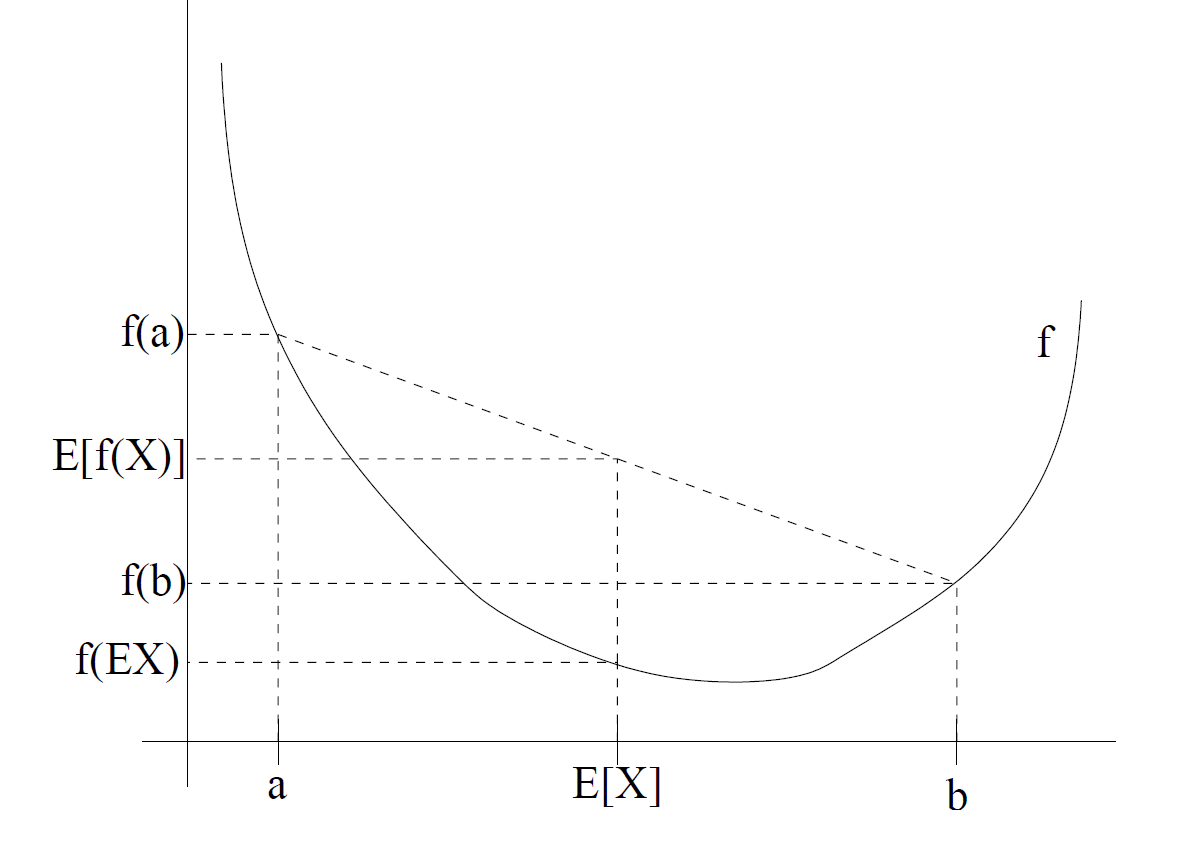
\includegraphics[width=0.55\textwidth]{jesen-inequality}
  \caption{Jensen's Inequality示例 \label{fig:jesen-inequality}}
\end{figure}

图中实线部分$f$是一个凸函数,随机变量$X$分别以$0.5$的概率取值$a$和$b$,因此随机变量$X$的期望为$a$和$b$的中间值,即:
\begin{align}
\label{eqn:exam-jsen}
  EX = \frac{a+b}{2}
\end{align}
期望对应的函数值为$f(EX)$,如图所示。而$E[f(X)]$等于:
\begin{align}
\label{eqn:exam-jsen1}
  E[f(X)] = \frac{f(a)+f(b)}{2}
\end{align}

从图上我们可以很明显的看出来二者的大小关系,又因为$X$是随机变量,当我们取$X=EX$的时候,函数的期望$E[f(x)]$和期望的函数$f(EX)$是相等的,所以有定理\ref{thm:jensen-ineq}。

\subsection{EM算法推导}
一般地,用$X$表示观测随机变量的数据,$Z$表示隐随机变量的数据,$X$和$Z$连在一起称为完全数据。观测数据$X$又称为不完全数据。假设给定观测数据$X$,其概率分布是$P(X|\theta)$,其中$\theta$是需要估计的参数,那么不完全数据$X$的似然函数是$P(X|\theta)$,对数似然函数是$L(\theta)=\log P(X|\theta)$;假设$X$和$Z$的联合概率分布是$P(X,Z|\theta)$,那么完全数据的对数似然函数是$L(\theta)=\log P(X,Z|\theta)$。

假设有$m$个相互独立的训练样本$\{x^{(1)},...,x^{(m)}\}$,我们需要估计这$m$个样本概率分布的参数。若隐变量为$z$,想要找到拟合模型$p(x,z)$的参数,其对数似然函数如公式\ref{eqn:em-likelihood}。
\begin{align}
\label{eqn:em-likelihood}
\begin{split}
  l(\theta) &= \sum_{i=1}^{m} \logp(x_{(i)}; \theta) \\
            &= \sum_{i=1}^{m} \log \sum_{z} p(x_{(i)}|z;\theta)p(x;\theta) \\
            &= \sum_{i=1}^{m} \log \sum_{z} p(x^{(i)}, z;\theta)
\end{splits}
\end{align}

由于隐变量$z$的存在,导致很难使用最大似然估计来得到参数$\theta$,在这种情况下,EM算法做的事情是给似然函数找个下界(E步),然后最大化这个下界(M步),如此反复迭代多次,最终收敛为止。

对于每一个样本$x^{(i)}$,我们定义$Q_{i}$为隐随机变量$z$的分布,其满足:
\begin{align}
\label{eqn:z-dis}
  \sum_{z} Q_{i}(z) = 1, \  Q_{i}(z) \geq 0
\end{align}
下面,我们来推导一下EM算法的精髓过程,见公式\ref{eqn:em-tuidao}。
\begin{align}
\label{eqn:em-tuidao}
\begin{split}
  \sum_{i=1}^{m} \logp(x_{(i)}; \theta) 
            &= \sum_{i=1}^{m} \log \sum_{z^{(i)}} p(x^{(i)}, z;\theta) \\
            &= \sum_{i=1}^{m} \log \sum_{z^{(i)}} Q_{i}(z^{(i)}) \frac{p(x^{(i)}, z;\theta)}{Q_{i}(z^{(i)})} \\
            &\geq \sum_{i=1}^{m} \sum_{z^{(i)}}  Q_{i}(z^{(i)}) \log \frac{p(x^{(i)}, z;\theta)}{Q_{i}(z^{(i)})}
\end{split}
\end{align}

公式\ref{eqn:em-tuidao}的最后一步是通过Jensen's Inequality得到的。我们分析下这个推导。

首先我们知道对数函数为凹函数,因为对数函数的二阶导$f^{''}(x)=-1/x^{2}<0$,其中$x\in{R^{+}}$。而
\begin{align}\nonumber
\label{eqn:em-expe}
\sum_{z^{(i)}} Q_{i}(z^{(i)}) \frac{p(x^{(i)}, z;\theta)}{Q_{i}(z^{(i)})}
\end{align}
是
\begin{align}\nonumber
\label{eqn:em-expe1}
\frac{p(x^{(i)}, z;\theta)}{Q_{i}(z^{(i)})}
\end{align}
关于服从分布$Q_{i}$的随机变量$z_{i}$期望。

由Jensen's Inequality可以得到公式\ref{eqn:em-jensen}:
\begin{align}
\label{eqn:em-jensen}
f\Bigg(E_{z^{(i)}\sim Q_{i}}\Big [\frac{p(x^{(i)}, z;\theta)}{Q_{i}(z^{(i)})}\Big ]\Bigg) \geq  E_{z^{(i)}\sim Q_{i}}\Bigg [f\Big(\frac{p(x^{(i)}, z;\theta)}{Q_{i}(z^{(i)})}\Big)\Bigg ]
\end{align}

其中下角标${z^{(i)}\sim Q_{i}}$表示这个期望是针对服从分布$Q_{i}$的随机变量$z^{(i)}$,根据公式\ref{eqn:em-jensen}就可以推出\ref{eqn:em-tuidao}的最后一步。

ok,关于公式\ref{eqn:em-jensen}多说两句,这里面其实用到的公式就是Jensen不等式,但是这个式子和前面我们提到的定理\ref{thm:jensen-ineq}中的区别在于$E[f(X)] \geq f(EX)$中的$X$同样是个函数,其等于:
\begin{align}\nonumber
\label{eqn:em-expe1}
\frac{p(x^{(i)}, z;\theta)}{Q_{i}(z^{(i)})}
\end{align}

以上公式\ref{eqn:em-tuidao}给$l{\theta}$提供了一个下界,我们不断地最大化这个下界,就可以不断地增加$l(\theta)$,说明每一次迭代模型都能找到拟合的更好的参数。

好的,下一个问题是,我们如何最大化这个下界呢?假设$t$轮迭代后的参数为$\theta^{(t)}$,我们希望通过这个$\theta^{(t)}$来得到$Q_{i}(z^{(i)})$,即隐变量的分布。而$t$轮迭代的时候一定是满足下界最大化的,而最大化很明显就是变不等号为等号的临界部分,即定理\ref{thm:jensen-ineq}中等号成立的条件。所以第$t$轮得到的$\theta^{(t)}$必然满足公式\ref{eqn:theta-1}。
\begin{align}
\label{eqn:theta-1}
E_{z^{(i)}\sim Q_{i}}\Big [\frac{p(x^{(i)}, z;\theta)}{Q_{i}(z^{(i)})}\Big ] = \frac{p(x^{(i)}, z;\theta)}{Q_{i}(z^{(i)})}
\end{align}
展开之后有:
\begin{align}
\label{eqn:theta-2}
\begin{split}
\sum_{z} Q_{i}(z^{(i)} \frac{p(x^{(i)}, z;\theta)}{Q_{i}(z^{(i)})}
    &= \sum_{z} p(x^{(i)}, z;\theta) \\
    &= \frac{p(x^{(i)}, z;\theta)}{Q_{i}(z^{(i)})}
\end{split}
\end{align}

所以我们有:
\begin{align}
\label{eqn:theta-2}
\begin{split}
  Q_{i}(z^{(i)}) &= \frac{p(x^{(i)}, z;\theta)}{\sum_{z} p(x^{(i)}, z;\theta)} \\
                 &= \frac{p(x^{(i)}, z;\theta)}{p(x^{(i)} ;\theta)} \\
                 &= p(z | x^{(i)};\theta)
\end{split}
\end{align}

上面的推导过程其实就是EM算法中的E步。

总结下EM算法步骤:
\begin{enumerate}
  \item E步:对于每一个样本,作:
    \begin{align}
    \label{eqn:estep}
      Q_{i} \coloneqq p(z | x^{(i)};\theta)
    \end{align}
  \item M步:
    \begin{align}
    \label{eqn:mstep}
      \theta \coloneqq \arg\mathop{\max}_{\theta} \sum_{i=1}^{m} \sum_{z^{(i)}}  Q_{i}(z^{(i)}) \log \frac{p(x^{(i)}, z;\theta)}{Q_{i}(z^{(i)})}
    \end{align}  
\end{enumerate}}

在用EM算法求模型参数的时候,首先定义模型的初始化参数,得到初始化参数之后,我们就可以得到隐随机变量$z$的分布,得到这个分布之后,我们再通过M步去算最大似然概率,得到新的参数,如此反复迭代,最终到EM算法收敛为止。

\subsection{EM算法收敛性证明}
如何证明EM算法最终一定会收敛呢?假设$\theta^{(t)}$和$\theta^{(t+1)}$为连续的两次迭代后的参数,我们只需要证明最大似然随着迭代次数是单调递增即可,即证明不等式\ref{eqn:em-conv}。
\begin{align}
\label{eqn:em-conv}
\theta^{(t+1)} \geq \theta^{(t)}
\end{align}

根据$t$轮迭代后的参数$\theta^{(t)}$,我们可以得到
\begin{align}\nonumber
\label{eqn:em-q}
Q_{i}^{(t)} = p(z | x^{(i)};\theta^{(t)})
\end{align}

那么$t$步的似然度为(此时公式\ref{eqn:em-tuidao}的最后一步取等号):
\begin{align}\nonumber
\label{eqn:em-like}
l(\theta^{(t)}) = \sum_{i=1}^{m} \sum_{z^{(i)}}  Q_{i}^{(t)}(z^{(i)}) \log \frac{p(x^{(i)}, z;\theta^{(t)})}{Q_{i}^{(t)}(z^{(i)})}
\end{align}

参数$\theta^{(t+1)}$则是通过最大化上述公式得到的。因此我们有:
\begin{align}
l(\theta^{(t+1)}) &\geq  \sum_{i=1}^{m} \sum_{z^{(i)}}  Q_{i}^{(t)}(z^{(i)}) \log \frac{p(x^{(i)}, z;\theta^{(t+1)})}{Q_{i}^{(t)}(z^{(i)})} \label{eqn:em-1} \\
                  &\geq  \sum_{i=1}^{m} \sum_{z^{(i)}}  Q_{i}^{(t)}(z^{(i)}) \log \frac{p(x^{(i)}, z;\theta^{(t)})}{Q_{i}^{(t)}(z^{(i)})} \label{eqn:em-2} \\
                  &= l(\theta^{(t)})  \label{eqn:em-3}
\end{align}

不等式\ref{eqn:em-1}是由公式\ref{eqn:em-tuidao}推导出来的,其对于任意的$Q_{i}$和$\theta$都是成立的,自然对于$Q_{i}=Q_{i}^{(t)}$和$\theta=\theta^{(t)}$也成立。而不等式\ref{eqn:em-2}是通过EM算法中的M步得到的,因为:
\begin{align}
  \theta^{(t+1)} = \arg\mathop{\max}_{\theta} \sum_{i=1}^{m} \sum_{z^{(i)}}  Q_{i}^{(t)}(z^{(i)}) \log \frac{p(x^{(i)}, z;\theta)}{Q_{i}^{(t)}(z^{(i)})}
\end{align}  

公式\ref{eqn:em-3}即为Jensen不等式处于临界条件时的结果。

由此可以得知$l(\theta)$是随着迭代次数的增加单调递增的,即似然度是单调收敛的。因此EM算法的终止条件是似然度收敛,即似然度不会再增加了为止。但是实际情况中一般是看两个相邻的迭代过程似然度的差是否低于一个预设的值,如果低于该值,则停止迭代。

定义公式\ref{eqn:jesen-1}:
\begin{align}
\label{eqn:jesen-1}
  J(Q,\theta) = \sum_{i=1}^{m} \sum_{z^{(i)}}  Q_{i}(z^{(i)}) \log \frac{p(x^{(i)}, z;\theta)}{Q_{i}(z^{(i)})}
\end{align}

我们知道$l(\theta) \geq J(Q,\theta)$,我们也可以把EM算法看成一个坐标上升的过程,在E步的时候,相当于固定$\theta$求$Q$;在M步的时候,相当于固定了$Q$求$\theta$。

{\bf 题外话:}这个固定一个变量,最大化另外一个变量,通过另外一个变量求这个变量这个思想感觉跟GAN很类似啊……GAN里面也是这样的,先固定生成器,优化判别器;然后固定判别器,优化生成器。有时间把这两个联系到一起来想想,还挺有意思的……
%------------------------------------------------------------------------------
%                                        GMM
%------------------------------------------------------------------------------
\section{混合高斯分布}

%方差
\begin{definition}{方差}{int}
方差用于描述数据的离散或波动程度。假定变量为$X$,均值为$\bar{X}$,$N$为总体样本数,方差计算公式如下:
\begin{align}
var(X) = \frac{\sum_{i=1}^{N}(X_i-\bar{X})^{2}}{N-1}
\end{align}
\end{definition}

%协方差
\begin{definition}{协方差}{int}
协方差表示了变量线性相关的方向,取值范围是$[-\infty, \infty]$,一般来说协方差为正值,说明一个变量变大另一个变量也变大;取负值说明一个变量变大另一个变量变小,取0说明两个变量没有相关关系.
\begin{align}
cov(X) = \frac{\sum_{i=1}^{N}(X_i-\bar{X})^{2}(Y_i-\bar{Y})^{2}}{N-1}
\end{align}
\end{definition}

%相关系数
\begin{definition}{相关系数}{int}
协方差可反映两个变量之间的相互关系及相关方向,但无法表达其相关的程度,皮尔逊相关系数不仅表示线性相关的方向,还表示线性相关的程度,取值$[-1,1]$,也就是说,相关系数为正值,说明一个变量变大另一个变量也变大;取负值说明一个变量变大另一个变量变小,取0说明两个变量没有相关关系,同时,相关系数的绝对值越接近1,线性关系越显著。
\begin{align}
\rho_{XY} = \frac{cov(X, Y)}{\sqrt{DX}\sqrt{DY}}
\end{align}
\end{definition}

%协方差矩阵
\begin{definition}{协方差矩阵}{int}
 当$X\in{R^{n}$为高维数据时,协方差矩阵可以很好的反映数据的性质,在协方差矩阵中,对角线元素反映了数据在各个维度上的离散程度,协方差矩阵为对角阵,非对角线元素反映了数据各个维度的相关性,其形式如下:
\begin{align}
\Sigma = 
\begin{bmatrix}
cov(x_1, x_1) & cov(x_1, x_2) & \cdots & cov(x_1, x_n) \\
cov(x_2, x_1) & cov(x_2, x_2) & \cdots & cov(x_2, x_n) \\
\vdots        & \vdots        & \ddots    & \vdots \\
cov(x_n, x_1) & cov(x_n, x_2) & \cdots & cov(x_n, x_n) 
\end{bmatrix}
\end{align}
\end{definition}

单变量高斯分布公式如\ref{eqn:gaussian},其中$\mu$和$\sigma^{2}$分别为均值和方差。
\begin{align}
\label{eqn:gaussian}
\mathcal{N}(x; \mu, \sigma) = \frac{1}{\sqrt{2\pi}\sigma}\exp{\{-\frac{(x-\mu)^{2}}{2\sigma^{2}}\}}
\end{align}

多变量高斯分布公式如\ref{eqn:mgaussian},其中$\mu$和$\Sigma$分别为均值和协方差矩阵。
\begin{align}
\label{eqn:mgaussian}
\mathcal{N}(x; \mu, \Sigma) = \frac{1}{(2\pi)^{-\frac{n}{2}}|\Sigma|^{\frac{1}{2}}}\exp{\{-\frac{1}{2}(x-\mu)^{T}\Sigma^{-1}(x-\mu)\}}
\end{align}

混合高斯模型(Gaussian Mixture Model)表示的是多个高斯分布叠加在一起的分布,其公式如\ref{eqn:GMM},其中$K$为高斯分量的个数,$\pi_{k}$为各个分量的权重,其满足$0 \leq \pi_{k} \leq 1$,且$\sum_{k=1}^{K}\pi_{k}=1$。$p(x)$表示的是多个高斯分量加权后的分布。
\begin{align}
\label{eqn:GMM}
p(x) = \sum_{k=1}^{K}\pi_{k}\mathcal{N}(x; \mu_{k}, \Sigma_{k})
\end{align}

那么给定一堆训练数据,我们如何根据这些数据来得到GMM的参数呢?

假设训练集$\{x^{(1)},...,x^{(m)}\}$,由于估计GMM的算法为无监督学习算法,因此这些数据都是没有标签的。我们用一个联合分布模型来对这些数据进行建模,即:
\begin{align}
p(x^{(i)}, z^{(i)})=p(x^{(i)}|z^{(i)})p(z^{(i)})
\end{align}
其中,$z^{i}\sim{Multinomial(\phi)}$,$s_{j} \geq 0$,且$\sum_{j=1}^{k} \phi_{j}=1$,$\phi_{j}$表示的是$p(z^{(i)}=j)$,此外$p(x^{(i)}|z^{(i)}=j)\sim{\mathcal{N}(\mu_j,\Sigma_j)}$。$k$表示的是$z^{(i)}$所能取的值的个数。

我们选取的模型假设每个$x^{(i)}$都由随机选取的$z^{(i)}$生成,$z^{(i)}\in\{1,...,k\}$。我们可以理解成GMM模型有$k$个高斯分量,$z$就是表征每个分量权重的随机变量,因此$z$就是隐变量。$p(z^{(i)})=\phi_{j}$就是$x^{(i)}$这个数据来源于分量$j$的概率。

综上,GMM模型的参数为$\mu,\Sigma,\phi$。现在的问题就是如何求解这些参数。我们可以得到似然函数如公式\ref{eqn:gmm-likelihood}。
\begin{align}
\label{eqn:gmm-likelihood}
\begin{split}
  l(\mu,\Sigma,\phi) 
      &= \sum_{i=1}^{m} \log p(x^{(i)};\mu,\Sigma,\phi) \\ 
      &= \sum_{i=1}^{m} \log \sum_{z_{(i)}=1}^{k} p(x^{(i)}|z^{(i)};\mu,\Sigma)p(z^{(i)};\phi)
\end{split}
\end{align}

如果我们直接对这个似然函数进行求导,由于隐变量的存在,我们无法得到关于参数的确切解。那么既然问题出在隐变量上,如果我们已经知道了每一个$x^{(i)}$所属的分量,公式\ref{eqn:gmm-likelihood}就可以写成公式\ref{eqn:gmm-likelihood1},需注意此时隐变量的分布我们还是不知道,我们只知道训练集中的样本分别属于哪一个高斯分量。
\begin{align}
\label{eqn:gmm-likelihood1}
\begin{split}
  l(\mu,\Sigma,\phi) 
        &= \sum_{i=1}^{m} \log p(x^{(i)}|z^{(i)};\mu,\Sigma)p(z^{(i)};\phi) \\
        &= \sum_{i=1}^{m} \Big[\log p(x^{(i)}|z^{(i)};\mu,\Sigma) + \log p(z^{(i)};\phi) \Big]
\end{split}
\end{align}

此时用最大似然概率求解的办法就可以得到这些参数,我们写细一点,求解一下看看。

首先,求解$\phi_j$,在此之前,我们可以看出$l$中与$\phi$相关的项为:
\begin{align}\nonumber
  \sum_{i=1}^{m} \log p(z^{(i)};\phi) 
\end{align}
我们知道$\phi$是服从多项式分布的,$\phi$受限于$\sum_{j=1}^{k} \phi_{j}=1$,因此关于$\phi$的求解我们需要构建一个拉格朗日函数如下:
\begin{align}\nonumber
      \mathcal{L}(\phi) = \sum_{i=1}^{m} \log p(z^{(i)};\phi) + \beta(\sum_{j=1}^{k} \phi_{j}-1)
\end{align}

因此关于求解$\phi$的步骤如公式\ref{eqn:gmm-phi1}:
\begin{align}
\label{eqn:gmm-phi1}
\begin{split}
  \frac{\partial \mathcal{L}(\phi)}{\partial \phi_j}
  &=\frac{\partial \sum_{i=1}^{m} \log p(z^{(i)};\phi) + \beta(\sum_{j=1}^{k} \phi_{j}-1)}{\partial \phi_j} \\
  &= \sum_{i=1}^{m} \frac{\partial \log p(z^{(i)};\phi)}{\partial \phi_j} \\
\end{split}
\end{align}

因为不一定每个$x^{(i)}$都有$j$分量产生,我们定义$1\{z^{(i)}=j\}$如下,也就是说第$i$个样本由第$j$个样本产生的时候,我们取为1。
\begin{equation}
1\{z^{(i)}=j\}=\left\{
\begin{array}{rcl}
1& & if \  z^{(i)}=j\\
0 & & otherwise\\
\end{array} \right.
\end{equation}

公式\ref{eqn:gmm-phi1}可以写成公式\ref{eqn:gmm-phi2}:
\begin{align}
\label{eqn:gmm-phi2}
\begin{split}
  \frac{\partial \mathcal{L}(\phi)}{\partial \phi_j}
  &=\frac{\partial \sum_{i=1}^{m} \log p(z^{(i)};\phi) + \beta(\sum_{j=1}^{k} \phi_{j}-1)}{\partial \phi_j} \\
  &= \sum_{i=1}^{m} 1\{z^{(i)}=j\} \frac{\partial \log \phi_j + \beta{\phi_{j}}}{\partial \phi_j} \\
  &= \sum_{i=1}^{m} 1\{z^{(i)}=j\} \Big[ \frac{1}{\phi_j} + \beta \Big]\\
\end{split}
\end{align}

令公式\ref{eqn:gmm-phi2}为0,解得:
\begin{align}
  \phi_j = \frac{\sum_{i=1}^{m} 1\{z^{(i)}=j\}}{-\beta}
\end{align}

由此可知:$\phi_j \propto \sum_{i=1}^{m} 1\{z^{(i)}=j\}$,又因为$\sum_{j=1}^{k} \phi_{j}=1$,将$\phi_j$代入约束条件有:
\begin{align}
  \sum_{j=1}^{k} \phi_j = \frac{ \sum_{j=1}^{k} \sum_{i=1}^{m} 1\{z^{(i)}=j\}}{-\beta} =1
\end{align}
即
\begin{align}
  -\beta = \sum_{j=1}^{k} \sum_{i=1}^{m} 1\{z^{(i)}=j\}
\end{align}
也就是说$-\beta$等于属于各个高斯分量的训练样本的和,也就是$m$。至此,我们可以得到如下公式:
\begin{align}
  \phi_j = \frac{1}{m}\sum_{i=1}^{m} 1\{z^{(i)}=j\}
\end{align}

接着我们来求$\mu$,如公式\ref{eqn:gmm-mu}。
\begin{align}
\label{eqn:gmm-mu}
\begin{split}
  \frac{\partial l(\mu,\Sigma,\phi)}{\partial \mu_j}
  &=\frac{\partial \sum_{i=1}^{m} \Big[\log p(x^{(i)}|z^{(i)};\mu,\Sigma) + \log p(z^{(i)};\phi) \Big]}{\partial \mu_j} \\
  &= \frac{\partial \sum_{i=1}^{m}\log p(x^{(i)}|z^{(i)};\mu,\Sigma)}{\partial \mu_j} \\
  &= \frac{\partial \sum_{i=1}^{m} 1\{z^{(i)}=j\} \log p(x^{(i)}|z^{(i)};\mu,\Sigma)}{\partial \mu_j} \\
  &= \frac{\partial \sum_{i=1}^{m} 1\{z^{(i)}=j\} \log{\mathcal{N}(x^{(i)}; \mu_j, \Sigma_j)} }{\partial \mu_j} \\
  &= \frac{\partial \sum_{i=1}^{m} 1\{z^{(i)}=j\} \log \frac{1}{(2\pi)^{-\frac{n}{2}}|\Sigma_j|^{\frac{1}{2}}} \exp{\{-\frac{1}{2}(x^{(i)}-\mu_j)^{T}\Sigma_j^{-1}(x^{(i)}-\mu_j)\}} }{\partial \mu_j} \\
  &= \frac{\partial \sum_{i=1}^{m} 1\{z^{(i)}=j\} [-\frac{1}{2}(x^{(i)}-\mu_j)^{T}\Sigma_j^{-1}(x^{(i)}-\mu_j)]}{\partial \mu_j} \\
  &= \frac{\partial \sum_{i=1}^{m} 1\{z^{(i)}=j\} [-\frac{1}{2}({x^{(i)}}^{T}\Sigma_j^{-1}{x^{(i)}} - \mu_j^{T}\Sigma_j^{-1}x^{(i)} - {x^{(i)}}^{T}\Sigma_j^{-1}\mu_j + \mu_j^{T}\mu_j)]}{\partial \mu_j} \\
  &= \frac{\partial \sum_{i=1}^{m} 1\{z^{(i)}=j\} [-\frac{1}{2}(-\mu_j^{T}\Sigma_j^{-1}{x^{(i)}} - {x^{(i)}}^{T}\Sigma_j^{-1}\mu_j + \mu_j^{T}\mu_j)]}{\partial \mu_j} \\
  &= \sum_{i=1}^{m} 1\{z^{(i)}=j\}\Sigma_j^{-1} ( {x^{(i)}} - \mu_j) 
\end{split}
\end{align}

令公式\ref{eqn:gmm-mu}为零,则有:
\begin{align}
\label{eqn:gmm-mu1}
\sum_{i=1}^{m} 1\{z^{(i)}=j\}\Sigma_j^{-1} ({x^{(i)}} - \mu_j) = 0
\end{align}
解得:
\begin{align}
\label{eqn:gmm-mu2}
\mu_j = \frac{\sum_{i=1}^{m} 1\{z^{(i)}=j\} x^{(i)}}{\sum_{i=1}^{m} 1\{z^{(i)}=j\}}
\end{align}
最后,根据方差的定义,我们可以计算出方差的值,如公式\ref{eqn:gmm-sigma}
\begin{align}
\label{eqn:gmm-sigma}
\Sigma_j = \frac{\sum_{i=1}^{m} 1\{z^{(i)}=j\} (x^{(i)}-\mu_j)(x^{(i)}-\mu_j)^{T}}{\sum_{i=1}^{m} 1\{z^{(i)}=j\}}
\end{align}

上面我们算了一下在已知每个样本所属的高斯分量的情况下参数$\phi,\mu,\Sigma$的估计值。回到最初那个问题,训练数据是没有标签的,那么怎么估计参数?

只要知道了每一个训练样本所属的高斯分量,我们就可以通过最大似然估计求出参数。既然如此,我们可以先随机的将训练样本进行分配,初始化时,随机指定每一个训练样本所属的高斯分量,结合\ref{sec:em}中讲的EM算法,我们可以算出$\phi,\mu,\Sigma$,再用这个参数来更新每一个样本所属的高斯分量,因为在得到参数后,我们将训练样本$x^{(i)}$代入到GMM中,可以得到该样本分别属于每一个高斯分量的概率值,即求取$p(z^{(i)}=j|x^{(i)};\phi,\mu,\Sigma), j\in\{1,...K\}$。得到这些概率之后,我们认为每一个高斯分量以权重$p(z^{(i)}=j|x^{(i)};\phi,\mu,\Sigma)$生成了样本$x^{(i)}$,知道这些权重之后就可以继续更新参数,这样往往复复,不停的迭代,就会不停的朝着正确分类的方向走去,最终收敛即可。

下面介绍下GMM参数估计的EM算法:
\begin{enumerate}
  \item E步:对于$i,j$,作:
    \begin{align}
    \label{eqn:gmm-estep}
      w_j^{(i)} \coloneqq p(z^{(i)}=j | x^{(i)};\phi, \mu, \Sigma)
    \end{align}
  \item M步:
    \begin{align}
    \label{eqn:gmm-mstep}
      \phi_j &\coloneqq \frac{1}{m}\sum_{i=1}^{m} w_j^{(i)} \\
      \mu_j  &\coloneqq \frac{\sum_{i=1}^{m} w_j^{(i)} x^{(i)}}{\sum_{i=1}^{m} w_j^{(i)}}  \\
      \Sigma &\coloneqq \frac{\sum_{i=1}^{m} w_j^{(i)} (x^{(i)}-\mu_j)(x^{(i)}-\mu_j)^{T}}{\sum_{i=1}^{m} w_j^{(i)}}
    \end{align}  
\end{enumerate}}
%------------------------------------------------------------------------------
%                                      HMM
%------------------------------------------------------------------------------
\section{HMM相关知识点总结}
本节笔记来自于CS229课程中Daniel Ramage的Hidden Markov Models Fundamentals\upcite{hmm-cs229}。
\subsection{Markov Models}
给定状态集合$S=\{s_1, s_2, ..., s_{|S|}\}$,我们可以观测到沿着时间线的序列$\vec{z}\in S^{T}$。比方说一个天气系统$S=\{sun, cloud, rain\}$,其$|S|=3$。假设连续五天观察到的天气序列为$\{z_1=s_{sun}, z_2=s_{cloud}, z_3=s_{cloud}, z_4=s_{rain}, z_5=s_{cloud}\}$。

上述天气系统中观测到的状态序列是时间线上的随机过程,如果不作进一步假设的话,$t$时刻的状态$s_j$可能是任意变量的函数,不仅仅包括从时刻$1$到时刻$t-1$的状态,甚至还包括一些没有建模的变量,所以我们作出两个{\bf Markov Assumptions}使模型更可行:
\begin{enumerate}
  \item {\bf Limited Horizon Assumption}:假设$t$时刻的处于某个状态的概率只取决于$t-1$时刻的状态。本假设的直观感受是:$t-1$时刻的状态囊括了对过去时刻状态的总结,因而可以用于预测$t$时刻的输出。即:
    \begin{align}
      \label{eqn:lha}
      P(z_t|z_{t-1}, z_{t-2}, ..., z_1) = P(z_t|z_{t-1})
    \end{align}
  \item {\bf Stationary Process Assumption}:给定当前状态,下一个时刻的状态分布不随着时间变化而变化。即:
    \begin{align}
      \label{eqn:spa}
      P(z_t|z_{t-1}) = P(z_2|z_1)
    \end{align}
    其中$z_{t-1}=z_1$。
\end{enumerate}

按照惯例,我们假设存在初始状态和初始观测$z_0\equiv s_0$,$s_0$表示的是在$t=0$处的初始概率分布。这么表达初始状态方便我们计算第一个真实状态的先验概率为$P(z_1|z_0)$,且可以得到$P(z_t|z_{t-1},...,z_1)=P(z_t|z_{t-1},...,z_1,z_0)$。此外,也有表达方式将这些先验置信度表示为$\pi \in R^{|S|}$。

我们定义一个状态转移矩阵$A\in{R^{(|S|+1)\times(|S|+1)}}$来表示各个状态之间的转移,其中$A_{ij}$表示的是任意时刻从状态$i$转移到状态$j$的概率。对于上述提到的天气系统,其转移矩阵可能如下:
\begin{align}
A = 
\begin{matrix}
            & s_0   &  s_{sun} & s_{cloud}  & s_{rain} \\
 s_0        & 0     &  0.33    & 0.33       & 0.33      \\
 s_{sun}    & 0     &  0.8     & 0.1        & 0.1       \\
 s_{cloud}  & 0     &  0.2     & 0.6        & 0.2      \\
 s_{rain}   & 0     &  0.1     & 0.2        & 0.7      
\end{matrix}
\end{align}

上面这个编出来的矩阵说明了天气是自我关联的,如果今天是晴天,明天还是晴天的概率会比较大;如果今天多云,明天还是多云的概率就比较大。这个规律在很多Markov Model里都有,从转移矩阵的对角线上也可以看出来。在这个天气系统中,初始化天气是均匀分布的。

\subsection{Markov Model的两个基本问题}
将上节中讲到的{\bf Markov Assumption}和状态转移矩阵$A$结合起来,我们就可以回答Markov Chain中关于状态序列的两个基本问题了。
\begin{itemize}
  \item 给定一个状态序列$\vec{z}$,如何求这个序列的概率?
  \item 如何通过最大化一个观测序列$\vec{z}$的似然概率来估计模型的参数?
\end{itemize}

\subsubsection{状态序列的概率}
给定一个状态序列$\vec{z}$,其长度为$t$。我们通过概率的链式法则(Chain Rule)来求这个状态序列出现的概率,如公式\ref{eqn:markov-chain}。
\begin{align}
\label{eqn:markov-chain}
\begin{split}
  P(\vec{z}) &= P(z_{t}, z_{t-1}, ...,z_{1};A) \\
             &= P(z_{t}, z_{t-1}, ...,z_{1}, z_{0};A) \\
             &= P(z_{t}|z_{t-1}, ...,z_{1}, z_{0};A)P(z_{t-1}|z_{t-2}, ...,z_{1}, z_{0};A)...P(z_1|z_0;A) \\
             &= P(z_{t}|z_{t-1};A)P(z_{t-1}|z_{t-2};A)...P(z_1|z_0;A) \\
             &= \prod_{t^{'}=1}^{t} P(z_{t^{'}}|z_{t^{'}-1};A)  \\
             &= \prod_{t^{'}=1}^{t} A_{z_{t^{'}-1}z_{t^{'}}}
\end{split}
\end{align}

根据公式\ref{eqn:markov-chain},我们可以求一下上节中提到的天气序列的概率:
\begin{align}
\label{eqn:markov-chain-example}
\begin{split}
&P(z_1=s_{sun}, z_2=s_{cloud}, z_3=s_{cloud}, z_4=s_{rain}, z_5=s_{cloud}) \\
      &= P(s_{sun}|s_0)P(s_{cloud}|s_{sun})P(s_{cloud}|s_{cloud})P(s_{rain}|s_{cloud})P(s_{cloud}|s_{rain}) \\
      &= 0.33 \times 0.1 \times 0.2 \times 0.7 \times 0.2 \\
      &= 0.000924‬
\end{split}
\end{align}

\subsubsection{Markov Model的最大似然估计}
出于学习的目的,我们希望找到参数$A$能够最大化长度为$T$的观测序列$\vec{z}$的最大对数似然。比方说求出天气系统中的从sunny转移到cloudy或者从sunny转移到sunny的概率等等,以使得观测序列最有可能出现。定义对数似然函数如公式\ref{eqn:markov-likelihood}。
\begin{align}
\label{eqn:markov-likelihood}
\begin{split}
  l(A) &= \log P(\vec{z};A) \\
       &= \log \prod_{t=1}^{T} A_{z_{t-1}z_t} \\
       &= \sum_{t=1}^{T} \log A_{z_{t-1}z_t} 
\end{split}
\end{align}

我们要估计的是$A$,所以我们需要将$A$的每一个元素$A_{ij}$都呈现在对数似然函数中,可是就从公式\ref{eqn:markov-likelihood}中,我们没法呈现$A_{ij}$。当然$\vec{z}$是已知的,即每个时刻的状态是确定的,但是我们没办法直接去指定$\vec{z}$中的每一个元素去估计$A$,因为我们希望得到的是一般意义的最大似然函数,即不论$\vec{z}$中都有哪些状态,公式\ref{eqn:markov-likelihood}都可以表示针对样本序列$\vec{z}$的最大似然函数。因此我们可以定义一个{\bf indicator function}如公式\ref{eqn:markov-indicator}(这个函数在GMM那一讲中也出现过)。
\begin{equation}
\label{eqn:markov-indicator}
1\{z_t=j \wedge z_{t-1}=i\}=\left\{
\begin{array}{rcl}
1& & if \  z_t=j \  and \  z_{t-1}=i\\
0 & & otherwise\\
\end{array} \right.
\end{equation}

这个函数的意义是当$t-1$时刻状态为$i$,并且$t$时刻状态为$j$,其取值为1。这样就和$A_{ij}$对应起来了,而且无需担心观测序列$\vec{z}$中是否有前一时刻为$i$、当前时刻为$j$的存在。那么我们可以继续推导公式\ref{eqn:markov-likelihood},即枚举所有可能出现的序列,而对应的状态序列是否存在则由$\vec{z}$来决定,如果某个状态转移存在,那么其状态转移的概率就会被保留下来用于计算最大似然函数,如果不存在,那么其状态转移概率就会被扔掉。
\begin{align}
\label{eqn:markov-likelihood1}
\begin{split}
  l(A) &= \sum_{t=1}^{T} \log A_{z_{t-1}z_t} \\
       &= \sum_{i=1}^{|S|} \sum_{j=1}^{|S|} \sum_{t=1}^{T} 1\{z_t=j \wedge z_{t-1}=i\} \log A_{ij}
\end{split}
\end{align}

由于$1\{z_t=j \wedge z_{t-1}=i\}$的限制,公式\ref{eqn:markov-likelihood1}一定会迫使着最大似然函数是对应着观测序列$\vec{z}$的。

为了解决这个优化问题,我们需要保证最终求出来的转移矩阵$A$是有效的。那么针对每一个状态,从该状态跳转到下一个时刻状态的概率和应当等于1,当然,$A$中的每一个元素都必须是非负的。因此,我们用拉格朗日算子来解决这个问题,如公式\ref{eqn:markov-lage}。
\begin{align}
\label{eqn:markov-lage}
\begin{split}
    A &= \arg\mathop{\max}_{A}l(A)\\
s.t \sum_{j=1}^{|S|} A_{ij} &=1, i\in\{1,2,...,|S|\} \\
    A_{ij} &\geq 0, i,j \in  \{1,2,...,|S|\}
\end{split}
\end{align}

我们可以构造一个拉格朗日函数来解决这个受约束的最优化问题,如公式\ref{eqn:markov-lage1}。
\begin{align}
\label{eqn:markov-lage1}
\begin{split}
    \mathcal{L}(A) &= l(A) + \sum_{i=1}^{|S|} \alpha_{i}(1-\sum_{j=1}^{|S|} A_{ij}) \\
                   &= \sum_{i=1}^{|S|} \sum_{j=1}^{|S|} \sum_{t=1}^{T} 1\{z_t=j \wedge z_{t-1}=i\} \log A_{ij} + \sum_{i=1}^{|S|} \alpha_{i}(1-\sum_{j=1}^{|S|} A_{ij}) 
\end{split}
\end{align}

求偏微分并置0,有:
\begin{align}
\label{eqn:markov-grad}
\begin{split}
    \frac{\partial \mathcal{L}(A)}{\partial A_{ij}}
          &=  \frac{\partial \sum_{i=1}^{|S|} \sum_{j=1}^{|S|} \sum_{t=1}^{T} 1\{z_t=j \wedge z_{t-1}=i\} \log A_{ij} + \sum_{i=1}^{|S|} \alpha_{i}(1-\sum_{j=1}^{|S|} A_{ij})}{\partial A_{ij}} \\
          &= \frac{1}{A_{ij}} \sum_{t=1}^{T} 1\{z_t=j \wedge z_{t-1}=i\} + \alpha_i \\
          &= 0
\end{split}
\end{align}

解得:
\begin{align}
\label{eqn:markov-grad1}
   A_{ij} = \frac{1}{\alpha_i}\sum_{t=1}^{T} 1\{z_t=j \wedge z_{t-1}=i\}
\end{align}

又因为:
\begin{align}
  \sum_{j=1}^{|S|} A_{ij} &=1, i\in\{1,2,...,|S|\} \\
\end{align}

代入公式\ref{eqn:markov-grad1}求得的$A_{ij}$有:
\begin{align}
  \sum_{j=1}^{|S|} \frac{1}{\alpha_i}\sum_{t=1}^{T} 1\{z_t=j \wedge z_{t-1}=i\} = 1
\end{align}
解得:
\begin{align}
\begin{split}
\alpha_i  &= \sum_{j=1}^{|S|} \sum_{t=1}^{T} 1\{z_t=j \wedge z_{t-1}=i\} \\
          &=  \sum_{t=1}^{T} 1\{z_{t-1}=i\}
\end{split}
\end{align}
所以:
\begin{align}
\label{eqn:markov-grad2}
   A_{ij} = \frac{\sum_{t=1}^{T} 1\{z_t=j \wedge z_{t-1}=i\}}{\sum_{t=1}^{T} 1\{z_{t-1}=i\}}
\end{align}

以上为Markov Model在已知观测序列的条件下估计状态转移矩阵$A$的推导。从公式\ref{eqn:markov-grad2}中,我们可以直观的看到$A_{ij}$就等于观测序列中,状态$i$跳转到状态$j$的次数除以位于状态$i$的个数。

\subsection{Hidden Markov Model}
\label{sub:hmm}
Markov Model是处理时序数据的一大利器,但是有些时候我们是无法观测状态序列的,在这种情况下,Markov Model就无法使用了。在状态序列无法观测的情况下,我们知道这些状态的概率函数,那么如何利用这些状态序列的概率函数来对模型建模呢?比如说语音识别中的,我们能观测到的是根据词发出的声音,但是其对应的词我们是不知道的,如何根据这些声音的声学特征来估计对应的词呢?

为了介绍HMM,我们借用下Jason Eisner论文中提出的“Ice Cream Climatology”\upcite{ice-cream-climatology},此处附上原文:

\begin{quotation}
The situation: You are a climatologist in the year 2799, studying the history of global warming. You can't find any records of Baltimore weather, but you do find my (Jason Eisner's) diary, in which I assiduously recorded how much ice cream I ate each day. What can you figure out from this about the weather that summer?
\end{quotation}

我们可以用HMM来解决这个问题。这个问题中模型的状态的序列(每一天的天气)是未知的,我们只能够观测到状态的输出序列(每天吃多少冰淇淋)。

正式地,HMM是一种Markov Model,其有一系列的观测输出$x=\{x_1, x_2, ..., x_T\}, x_t\in{V}, t=1,...,T$,其中$V=\{v_1, v_2, ..., v_{|V|}\}$为观测输出集合。同样有状态序列$z={z_1, z_2, .., z_T}, z_{t}\in{S}$,其中$S=\{s_1, s_2, ..., s_{|S|}\}$为状态的集合。在HMM中,状态是不可观测的。状态之间的转移概率仍然由状态转移矩阵$A$表示。

同时生成观测输出的概率为隐状态的函数。为了满足这个这个条件,我们假设HMM中所有的输出是相互独立的,且定义:
\begin{align}
   P(x_t=v_k|z_{t}=s_{j}) &= P(x_t=v_k|x_1,...,x_T,z_1,...,z_T) \\
                          &= B_{jk}
\end{align}

矩阵$B$表示的是在某个时刻处于状态$s_j$生成观测$v_k$的概率值。

回归到上面讲的天气例子,假设有连续四天的冰淇淋消耗量的日志$\vec{x}=\{x_1=v_3, x_2=v_2, x_3=v_1, x_4=v_2\}$,对应的$V=\{v_1=1 ice cream, v_2=2 ice creams, v_3=3 ice creams\}$。那么我们要解决HMM的哪些问题呢?

\subsection{HMM的三个基本问题}
HMM有三个基本问题,
\begin{itemize}
  \item 某个特定观测序列的概率值为多少(我们有多大的可能性看到连续四天消耗冰淇淋的量为 3,2,1,2)?
  \item 生成某个特定观测序列的最有可能的状态序列是什么(那四天的冰淇淋消耗量对应的状态序列是多少)?
  \item 给定一些观测序列,怎么去估计HMM的参数$A$和$B$?
\end{itemize}

\subsubsection{概率计算问题}
概率计算问题指的是已知观测序列,求的是HMM模型输出该观测序列的概率值,此时,状态转移矩阵$A$和发射矩阵$B$都是已知的。

在HMM中,数据生成的过程如下:

假定状态序列$\vec{z}$由一个Markov Model生成,其状态转移矩阵为$A$。在每一个时间步$t$,我们选定输出$x_t$,$x_t$是关于$z_t$的函数。为了得到观测序列的概率,给定每一个可能的观测序列,我们需要加上数据$\vec{x}$的似然度,见公式\ref{eqn:hmm-likelihood}
\begin{align}
\label{eqn:hmm-likelihood}
\begin{split}
  P(\vec{x};A,B) &= \sum_{\vec{z}} P(\vec{x},\vec{z};A, B) \\
                 &= \sum_{\vec{z}} P(\vec{x}|\vec{z};A,B) P(\vec{z};A;B)
\end{split}
\end{align}

公式\ref{eqn:hmm-likelihood}对于任意概率分布都成立;然而HMM的假设简化这个表达式,如公式\ref{eqn:hmm-likelihood1}。
\begin{align}
\label{eqn:hmm-likelihood1}
\begin{split}
  P(\vec{x};A,B) &= \sum_{\vec{z}} P(\vec{x}|\vec{z};A,B) P(\vec{z};A;B) \\
                 &= \sum_{\vec{z}} (\prod_{t=1}^{T} P(x_t|z_t; B)) (\prod_{t=1}^{T} P(z_t|z_{t-1};A)) \\
                 &= \sum_{\vec{z}} (\prod_{t=1}^{T} B_{z_{t}x_{t}})(\prod_{t=1}^{T} A_{z_{t-1}z_{t}})
\end{split}
\end{align}

在参数已知的情况下,公式\ref{eqn:hmm-likelihood1}是一个比较简单的表达式。HMM有三大假设:
\begin{itemize}
  \item output independent assumption;
  \item markov assumption;
  \item stationary process assumption.
\end{itemize}

但是在计算公式\ref{eqn:hmm-likelihood1}的过程中,由于求和是针对每一个可能的$\vec{z}$的,而任意时刻的$z_t$可以取$|S|$个值,计算上述的求和需要$O(|S|^{T})$次操作。一般我们使用一种动态规划算法:前后向算法来计算$P(\vec{x};A,B)$。

前向算法定义$\alpha_{i}(t)=P(x_1,x_2,...,x_t,z_t=s_i;A,B)$,$\alpha_t$表示的是直到$t$时刻的观测序列的概率值,且此时的状态为$s_i$。那么观测序列的概率值为:
\begin{align}
\label{eqn:hmm-likelihood2}
\begin{split}
  P(\vec{x};A,B) &= P(x_1,x_2,...,x_T;A,B) \\
                 &= \sum_{i}^{|S|} P(x_1,x_2,...,x_T,z_T=s_i;A,B) \\
                 &= \sum_{i}^{|S|} \alpha_{i}(T)
\end{split}
\end{align}

算法\ref{alg:hmm-forward}描述了前向算法的迭代过程,其提供了一个效率更高的方式来计算$\alpha_{i}(t)$。由算法可知,在每个时间步只需要进行$O(|S|)$次运算,最终计算出$P(\vec{x};A,B)$需要$O(|S|\dot T)$次运算。
\numberwithin{algorithm}{chapter}
\begin{algorithm}
\caption{HMM中的前向算法} 
\label{alg:hmm-forward}
\begin{enumerate}
  \item Base Case: $\alpha_{i}(0) = A_{0i}, i=1,2,...,|S|$;
  \item Recursion: $\alpha_{j}(t) = \sum_{i=1}^{|S|} \alpha_{i}(t-1)A_{ij}B_{jx_{t}}, j = 1,...,|S|, t=1,...,T$
\end{enumerate}
\end{algorithm}

类似的算法是后向算法,其定义后向概率$\beta_{i}(t)=P(x_T,x_{T-1},...,x_{t+1},z_t=s_i;A,B)$。我们同样可以得到:
\begin{align}
\label{eqn:hmm-likelihood2}
\begin{split}
  P(\vec{x};A,B) &= P(x_1,x_2,...,x_T;A,B) \\
                 &= \sum_{i}^{|S|} P(x_T,x_{T-1},...,x_1,z_0=s_i;A,B) \\
                 &= \sum_{i}^{|S|} \beta_{i}(0)
\end{split}
\end{align}

其复杂度与前向算法相同,如算法\ref{alg:hmm-backward}。
\numberwithin{algorithm}{chapter}
\begin{algorithm}
\caption{HMM中的后向算法} 
\label{alg:hmm-backward}
\begin{enumerate}
  \item Base Case: $\beta_{i}(T) = 1, i=1,2,...,|S|$;
  \item Recursion: $\beta_{j}(t) = \sum_{i=1}^{|S|} A_{ji}B_{jx_{t}}\beta_{i}(t+1), j = 1,...,|S|, t=1,...,T$
\end{enumerate}
\end{algorithm}

\subsubsection{预测问题}
HMM中最常见的一个问题是:给定观测序列$\vec{x}\in{V^{T}}$,最有可能产生$\vec{x}$的状态序列$\vec{x}$是什么?正式地:
\begin{align}
\arg\mathop{\max}_{\vec{z}} P(\vec{z}|\vec{x};A,B) 
&= \arg\mathop{\max}{\vec{z}} \frac{P(\vec{z},\vec{x};A,B)}{P(\vec{x};A,B)} \label{eqn:hmm-decode-1}\\
&= \arg\mathop{\max}{\vec{z}} \frac{P(\vec{x}, \vec{z};A,B)}{ \sum_{\vec{z}} P(\vec{x}, \vec{z};A,B)}  \label{eqn:hmm-decode-2} \\
&= \arg\mathop{\max}{\vec{z}} P(\vec{x}, \vec{z};A,B) \label{eqn:hmm-decode-3}
\end{align}

公式\ref{eqn:hmm-decode-1}和公式\ref{eqn:hmm-decode-2}利用的是贝叶斯定理和全概率公式,由公式\ref{eqn:hmm-decode-1}可知,其分母与$\vec{z}$无关,因此式\ref{eqn:hmm-decode-3}成立。我们可以尝试所有可能的$\vec{z}$,然后得到每一个$\vec{z}$的后验概率,选取其中最大值作为上述公式的解,然而这种解法同样需要$|S|^{T}$次操作。参考前面提到的前向算法,我们同样可以利用动态规划算法来求解$\vec{z}$。由于我们需要求解的是每一次迭代的最大值,而不是对每一个时间步求和,因此将$\sum_{\vec{z}}$替换成$\max$即可。我们称之为Viterbi算法,如算法\ref{alg:hmm-viterbi}。得到每一个时间步的最大概率状态序列,一直迭代到$T$为止,我们就得到了最有可能输出给定观测序列的状态序列。
\numberwithin{algorithm}{chapter}
\begin{algorithm}
\caption{HMM中的解码算法} 
\label{alg:hmm-viterbi}
\begin{enumerate}
  \item Base Case: $\alpha_{i}(0) = \max(A_{0i}), i=1,2,...,|S|$;
  \item Recursion: $\alpha_{j}(t) = \max(\alpha_{i}(t-1)A_{ij}B_{jx_{t}}), for\  i\  in\  \{1,2,...,|S|\} , j = 1,...,|S|, t=1,...,T$
\end{enumerate}
\end{algorithm}

\subsubsection{学习问题}
关于HMM,在给定一系列观测序列的条件下,如何去估计最有可能产生这些观测序列的状态转移矩阵$A$和发射概率矩阵$B$?比如说语音识别中,已知语音训练集,我们可以通过这些语音数据去训练HMM模型,估计出最适合的参数,从而可以利用这些参数去算未知语音的状态序列的最大似然。换大白话说一下这个例子:我们有一堆语音数据,这些数据的音频特征是已知的,这就是观测值,而对应的建模单元(音素什么的)是关于这些音频特征的函数,也就是状态值,我们希望通过这个训练数据来训练HMM模型,得到HMM的参数值,知道参数值之后,就可以用于识别其他音频了,这时候就变成了HMM的预测问题了。

所以如何通过训练集估计出模型的参数就变成了一个很重要的问题。本小节我们介绍一种EM算法的变体用于估计HMM的参数。算法\ref{alg:hmm-em1}。从算法中,我们可以看到M-Step有一些约束条件,这些约束条件保证了HMM的两个矩阵$A$和$B$的有效性。正如前面我们求解Markov Model的参数一样,对于这个这个优化问题需构建一个拉格朗日算子。可是不论是E-Step还是M-Step,都是对$S^{T}$内所有可能的状态序列$\vec{z}$进行枚举,E、M两步对于所有可能的标签序列(状态序列)$\vec{z}$都有$|S|^{T}$的复杂度。为了计算效率,同样使用前面提到的前后向算法来计算E、M两步的结果。
\begin{algorithm}
\caption{HMM中的EM算法1} 
\label{alg:hmm-em1}
\begin{algorithmic}[1]
  Repeat until convergence

  \{             

     (E-Step) For every possible labeling $\vec{z}\in{S^{T}}$, set 
     \begin{align}\nonumber
      Q(\vec{z}) \coloneqq p(\vec{z}|\vec{x};A,B)
     \end{align}

     (M-Step) Set 
     \begin{align}\nonumber
     \begin{split}
      A, B &\coloneqq \arg\mathop{\max}_{A,B}\sum_{\vec{z}}Q(\vec{z})\log\frac{P(\vec{z},\vec{x};A,B)}{Q(\vec{z})} \\
      s.t. &\sum_{j=1}^{|S|} A_{ij} = 1, i=1,2,...,|S|; A_{ij}\geq 0,i,j=1,2,...,|S|  \\
           &\sum_{k=1}^{|V|} B_{ik} = 1, i=1,2,...,|S|; B_{ik}\geq 0,i=1,...,|S|,k=1,...,|V|
      \end{split}
     \end{align}     
  \}
\end{algorithmic}
\end{algorithm}

首先让我们利用Markov Assumption重写估计HMM参数的目标函数,目标函数推导第二行是因为对数函数中的分母与所求的值无关,舍去了;第三行利用了Markov Assumption,而最后一行使用了{\bf indicator functions},这么表示之后,我们可以直接利用矩阵的索引来表示$A$和$B$。
\begin{align}
\label{eqn:hmm-obj}
\begin{split}
  A,B &= \arg\mathop{\max}_{A,B}\sum_{\vec{z}}Q(\vec{z})\log\frac{P(\vec{z},\vec{x};A,B)}{Q(\vec{z})} \\
      &= \arg\mathop{\max}_{A,B}\sum_{\vec{z}}Q(\vec{z})\log P(\vec{z},\vec{x};A,B) \\     
      &= \arg\mathop{\max}_{A,B}\sum_{\vec{z}}Q(\vec{z})\log \Big[ \prod_{t=1}^{T} p(\vec{z}_{t}|\vec{z}_{t-1};A) p(\vec{x}_{t}|\vec{z}_{t};B) \Big] \\
      &= \arg\mathop{\max}_{A,B}\sum_{\vec{z}}Q(\vec{z})\log \Big[ (p(\vec{z}_{t}|\vec{z}_{t-1};A))(\prod_{t=1}^{T} p(\vec{x}_{t}|\vec{z}_{t};B))  \Big] \\
      &= \arg\mathop{\max}_{A,B}\sum_{\vec{z}}Q(\vec{z})\sum_{t=1}^{T} \Big[\log{A_{z_{t-1}z_{t}}} + \log{B_{z_{t}x_{t}}} \Big] \\
      &= \arg\mathop{\max}_{A,B}\sum_{\vec{z}}Q(\vec{z})\sum_{i=1}^{|S|} \sum_{j=1}^{|S|} \sum_{k=1}^{|V|} \sum_{t=1}^{T} \Big[1\{z_{t-1}=s_i\wedge{z_t=s_j}\}\log{A_{ij}} + 1\{z_{t}=s_j\wedge{x_t=v_k}\}\log{B_{jk}} \Big]
\end{split}
\end{align}   

与前面求解Markov Model的最大似然估计一样,根据HMM的约束条件,我们构造一个拉格朗日函数,如公式\ref{eqn:hmm-lage},将约束条件包含到拉格朗日函数之后,这样我们就不需要担心这些不等式约束了,因为求解出来的值都是非负数。
\begin{align}
\label{eqn:hmm-lage}
\begin{split}
  \mathcal{L}(A,B,\delta,\epsilon) &= \sum_{\vec{z}}Q(\vec{z})\sum_{i=1}^{|S|} \sum_{j=1}^{|S|} \sum_{k=1}^{|V|} \sum_{t=1}^{T} \Big[1\{z_{t-1}=s_i\wedge{z_t=s_j}\}\log{A_{ij}} + 1\{z_{t}=s_j\wedge{x_t=v_k}\}\log{B_{jk}} \Big] \\
  &+ \sum_{j=1}{|S|}\epsilon_{j}(1-\sum_{k=1}^{|V|} B_{jk}) +  \sum_{i=1}{|S|}\delta_{i}(1-\sum_{j=1}^{|S|} A_{ij})
\end{split}
\end{align}  

公式\ref{eqn:hmm-lage}分别对HMM的参数矩阵中的各个元素求偏导数并置0。

对$A_{ij}$有:
\begin{align}
\label{eqn:hmm-a}
\begin{split}
\frac{\partial\mathcal{L}(A,B,\delta,\epsilon)}{\partial A_{ij}} &=\sum_{\vec{z}}Q(\vec{z})\frac{1}{A_{ij}}\sum_{t=1}^{T}1\{z_{t-1}=s_i\wedge{z_t=s_j}\} - \delta_{i} 
\end{split}
\end{align}  

置0解得:
\begin{align}
\label{eqn:hmm-a-answer}
A_{ij} =\frac{1}{\delta_{i}} \sum_{\vec{z}}Q(\vec{z})\sum_{t=1}^{T}1\{z_{t-1}=s_i\wedge{z_t=s_j}\}
\end{align}  

对$B_{jk}$有:
\begin{align}
\label{eqn:hmm-b}
\begin{split}
\frac{\partial\mathcal{L}(A,B,\delta,\epsilon)}{\partial B_{jk}} &=\sum_{\vec{z}}Q(\vec{z})\frac{1}{B_{jk}}\sum_{t=1}^{T}1\{z_{t}=s_i\wedge{x_t=v_k}\} - \epsilon_{j} 
\end{split}
\end{align}  

置0解得:
\begin{align}
\label{eqn:hmm-b-answer}
B_{jk} =\frac{1}{\epsilon_{j}} \sum_{\vec{z}}Q(\vec{z})\sum_{t=1}^{T}1\{z_{t}=s_j\wedge{x_t=v_k}\}
\end{align}  

再对拉格朗日算子中的参数求偏导,并代入上述求得的$A_{ij}$和$B_{jk}$。

对$\delta_{i}$有
\begin{align}
\label{eqn:hmm-delta}
\begin{split}
\frac{\partial\mathcal{L}(A,B,\delta,\epsilon)}{\partial \delta_{i}} 
        &= 1-\sum_{j=1}^{|S|} A_{ij}  \\
        &= 1-\sum_{j=1}^{|S|} \frac{1}{\delta_{i}} \sum_{\vec{z}}Q(\vec{z})\sum_{t=1}^{T}1\{z_{t-1}=s_i\wedge{z_t=s_j}\}
\end{split}
\end{align}  

置0解得:
\begin{align}
\label{eqn:hmm-delta-answer}
\begin{split}
\delta_{i} &= \sum_{j=1}^{|S|} \sum_{\vec{z}}Q(\vec{z})\sum_{t=1}^{T}1\{z_{t-1}=s_i\wedge{z_t=s_j}\} \\
           &= \sum_{\vec{z}}Q(\vec{z})\sum_{t=1}^{T}1\{z_{t-1}=s_i\}
\end{split}
\end{align} 

对$\epsilon_{i}$有
\begin{align}
\label{eqn:hmm-epsilon}
\begin{split}
\frac{\partial\mathcal{L}(A,B,\delta,\epsilon)}{\partial \epsilon_{i}} 
        &= 1-\sum_{k=1}^{|V|} B_{jk}  \\
        &= 1-\sum_{k=1}^{|V|} \frac{1}{\epsilon_{j}} \sum_{\vec{z}}Q(\vec{z})\sum_{t=1}^{T}1\{z_{t}=s_j\wedge{x_t=v_k}\}
\end{split}
\end{align}  

置0解得:
\begin{align}
\label{eqn:hmm-epsilon-answer}
\begin{split}
\epsilon_{i} &= \sum_{k=1}^{|V|} \sum_{\vec{z}}Q(\vec{z})\sum_{t=1}^{T}1\{z_{t}=s_j\wedge{x_t=v_k}\} \\
           &= \sum_{\vec{z}}Q(\vec{z})\sum_{t=1}^{T}1\{z_{t}=s_j\}
\end{split}
\end{align} 

再将$\delta_{i}$和$\epsilon_{j}$代回到公式\ref{eqn:hmm-a-answer}和公式\ref{eqn:hmm-b-answer}有:
\begin{align}
\label{eqn:hmm-a-b-answer}
\begin{split}
A_{ij} &= \frac{\sum_{\vec{z}}Q(\vec{z})\sum_{t=1}^{T}1\{z_{t-1}=s_i\wedge{z_t=s_j}\}}{\sum_{\vec{z}}Q(\vec{z})\sum_{t=1}^{T}1\{z_{t-1}=s_i\}} \\
B_{jk} &=\frac{\sum_{\vec{z}}Q(\vec{z})\sum_{t=1}^{T}1\{z_{t}=s_j\wedge{x_t=v_k}\}}{\sum_{\vec{z}}Q(\vec{z})\sum_{t=1}^{T}1\{z_{t}=s_j\}} 
\end{split}
\end{align} 

公式\ref{eqn:hmm-a-b-answer}中的$A_{ij}$和$B_{jk}$即为每一轮迭代中的M-Step所求,但是从公式上来看,都是对所有可能的标签序列$\vec{z}\in{S^{T}}$的枚举求和。前面提到的E-step中的$Q_{\vec{z}}$的定义是$P(\vec{z}|\vec{x};A,B)$。我们考虑下如何用前后向概率$\alpha_{i}(t)$和$\beta_{j}(t)$来表征参数$A_{ij}$中的分子:
\begin{align}
\begin{split}
 &\sum_{\vec{z}}Q(\vec{z})\sum_{t=1}^{T}1\{z_{t-1}=s_i\wedge{z_t=s_j}\} \\
 &= \sum_{t=1}^{T} \sum_{\vec{z}} 1\{z_{t-1}=s_i\wedge{z_t=s_j}\}Q(\vec{z}) \\
 &= \sum_{t=1}^{T} \sum_{\vec{z}} 1\{z_{t-1}=s_i\wedge{z_t=s_j}\}P(\vec{z}|\vec{x};A,B) \\
 &= \frac{1}{P(\vec{x};A,B)} \sum_{t=1}^{T} \sum_{\vec{z}} 1\{z_{t-1}=s_i\wedge{z_t=s_j}\}P(\vec{z},\vec{x};A,B) \\
 &= \frac{1}{P(\vec{x};A,B)} \sum_{t=1}^{T} \alpha_{i}(t)A_{ij}B_{jx_{t}}\beta_{j}(t+1)
\end{split}
\end{align}

解释下上面这个牛逼的公式。第二行和第三行是重新整理了下公式并且代入了$Q(\vec{z})$的定义。第四步是根据贝叶斯定理。第五步就是我个人认为非常吊的一步了。我们仔细看下$1\{z_{t-1}=s_i\wedge{z_t=s_j}\}$,这个式子的意思是$t$时刻处于状态$s_i$,$t+1$时刻处于$s_j$,好了,其他时刻,从$1$到$t-1$,从$t+2$到$T$,这些个时候处于什么状态,我们不在乎。是啥都可以。那么我们先来考虑下从$1$到$t$这个时间段,再配合上$\sum{\vec{z}},这不就是前向概率吗?换句话说,公式:
\begin{align}\nonumber
sum_{\vec{z}} 1\{z_{t-1}=s_i\wedge{z_t=s_j}\}P(\vec{z},\vec{x};A,B)
\end{align}
这就是前面我们提到的前后向概率,只不过由于此时有两个时刻的状态是确定的:$z_{t-1}=s_i$、$z_{t}=s_j$,一个从到$s_i$,一个是从$s_j$出发,前面就是终止状态为$s_i$的前向概率,后面就是初始状态为$s_j$的后向概率。

所以这个转换太厉害了。内心鼓掌……

……

同样分母可以转换成:
\begin{align}
\begin{split}
 &\sum_{\vec{z}}Q(\vec{z})\sum_{t=1}^{T}1\{z_{t-1}=s_i\} \\
 &=\sum_{t=1}^{T} \sum_{\vec{z}} 1\{z_{t-1}=s_i\}Q(\vec{z}) \\
 &=\sum_{t=1}^{T} \sum_{\vec{z}} 1\{z_{t-1}=s_i\}P(\vec{z}|\vec{x};A,B) \\ 
 &=\frac{1}{P(\vec{x};A,B)} \sum_{t=1}^{T} \sum_{\vec{z}} 1\{z_{t-1}=s_i\}P(\vec{z},\vec{x};A,B) \\
 &=\frac{1}{P(\vec{x};A,B)} \sum_{t=1}^{T} \alpha_{i}(t)A_{ij} \\
\end{split}
\end{align}

需要时刻谨记的是上述分子分母中的$A_{ij}$和$B_{jx_{t}}$都是上一轮迭代出来的参数,用于更新本轮参数,为了避免产生混淆,我们将本轮更新后的参数分别记作$\hat{A}_{ij}$和$\hat{B}_{jx_{t}}$。因此:
\begin{align}
 \hat{A}_{ij} = \frac{\sum_{t=1}^{T} \alpha_{i}(t)A_{ij}B_{jx_{t}}\beta_{j}(t+1)}{\sum_{t=1}^{T} \alpha_{i}(t)A_{ij}}
\end{align}

另外,此处说明一下,分母的计算与参考资料\upcite{hmm-cs229}中有些不同,其计算过程为:
\begin{align}
\begin{split}
 &\sum_{\vec{z}}Q(\vec{z})\sum_{t=1}^{T}1\{z_{t-1}=s_i\} \\
 &=\sum_{j=1}^{|S|} \sum_{t=1}^{T} \sum_{\vec{z}} 1\{z_{t-1}=s_i\wedge{z_t=s_j}\}Q(\vec{z}) \\
 &=\frac{1}{P(\vec{x};A,B)} \sum_{j=1}^{|S|}\sum_{t=1}^{T} \alpha_{i}(t)A_{ij}B_{jx_{t}}\beta_{j}(t+1)
\end{split}
\end{align}

最终求得的:
\begin{align}
 \hat{A}_{ij} = \frac{\sum_{t=1}^{T} \alpha_{i}(t)A_{ij}B_{jx_{t}}\beta_{j}(t+1)}{\sum_{j=1}^{|S|}\sum_{t=1}^{T} \alpha_{i}(t)A_{ij}B_{jx_{t}}\beta_{j}(t+1)}
\end{align}

同样地,$\hat{B}_{jk}$的分子可以转换如下:
\begin{align}
\begin{split}
 &\sum_{\vec{z}}Q(\vec{z})\sum_{t=1}^{T}1\{z_{t}=s_j\wedge{x_t=v_k}\} \\
 &= \sum_{t=1}^{T} \sum_{\vec{z}} 1\{z_{t}=s_j\wedge{x_t=v_k}\}Q(\vec{z}) \\
 &= \sum_{t=1}^{T} \sum_{\vec{z}} 1\{z_{t}=s_j\wedge{x_t=v_k}\}P(\vec{z}|\vec{x};A,B) \\
 &= \frac{1}{P(\vec{x};A,B)} \sum_{t=1}^{T} \sum_{\vec{z}} 1\{z_{t}=s_j\wedge{x_t=v_k}\} P(\vec{z};\vec{x};A,B) \\
 &= \frac{1}{P(\vec{x};A,B)} \sum_{i=1}^{|S|} \sum_{t=1}^{T} \sum_{\vec{z}} 1\{z_{t-1}=s_i\wedge z_{t}=s_j\wedge{x_t=v_k}\} P(\vec{z};\vec{x};A,B) \\
 &= \frac{1}{P(\vec{x};A,B)} \sum_{i=1}^{|S|} \sum_{t=1}^{T} 1\{x_t=v_k\} \alpha_{i}(t)A_{ij}B_{jx_{t}}\beta_{j}(t+1)
\end{split}
\end{align}

其分母可以转换为:
\begin{align}
\begin{split}
 &\sum_{\vec{z}}Q(\vec{z})\sum_{t=1}^{T}1\{z_{t}=s_j\} \\
 &= \sum_{t=1}^{T} \sum_{\vec{z}} 1\{z_{t}=s_j\}Q(\vec{z}) \\
 &= \sum_{t=1}^{T} \sum_{\vec{z}} 1\{z_{t}=s_j\}P(\vec{z}|\vec{x};A,B) \\
 &= \frac{1}{P(\vec{x};A,B)} \sum_{i=1}^{|S|} \sum_{t=1}^{T} \sum_{\vec{z}} 1\{z_{t-1}=s_i\wedge{z_t=s_j}\} P(\vec{z};\vec{x};A,B) \\
 &= \frac{1}{P(\vec{x};A,B)} \sum_{i=1}^{|S|} \sum_{t=1}^{T}\alpha_{i}(t)A_{ij}B_{jx_{t}}\beta_{j}(t+1)
\end{split}
\end{align}

故而:
\begin{align}
\hat{B}_{jk} = \frac{\sum_{i=1}^{|S|} \sum_{t=1}^{T} 1\{x_t=v_k\} \alpha_{i}(t)A_{ij}B_{jx_{t}}\beta_{j}(t+1)}{\sum_{i=1}^{|S|} \sum_{t=1}^{T}\alpha_{i}(t)A_{ij}B_{jx_{t}}\beta_{j}(t+1)}
\end{align}

算法\ref{alg:hmm-em2}描述了利用前后向算法来进行参数学习的Baum-Welch算法:
\begin{algorithm}
\caption{HMM中的Baum-Welch算法} 
\label{alg:hmm-em2}
\begin{algorithmic}[1]
Initialization: Set $A$ and $B$ as random valid probability matrices 

\quad where $A_{i0}=0$ and $B_{0k}=0$, for $i=1,...,|S|$ and $k=1,...,|V|$. \\

repeat until convergence \\
\{ \\

(E-Step) Run the forward-backward algorithms to compute $\alpha_i$ and $\beta_{j}$ for $i,j=1,...,|S|$\\
\begin{align} 
\label{eqn:gamma}
\gamma_{t}(i,j) \coloneqq \alpha_{i}(t)A_{ij}B_{jx_{t}}\beta_{j}(t+1)
\end{align}

(M-Step) Re-estimate the maximum likelihood parameters as: \\
\begin{align}
\label{eqn:hmm-a-b-answer-1}
\begin{split}
\hat{A}_{ij} &= \frac{\sum_{t=1}^{T} \gamma_{t}(i,j)}{\sum_{j=1}^{|S|}\sum_{t=1}^{T} \gamma_{t}(i,j)}\\
\hat{B}_{jk} &= \frac{\sum_{i=1}^{|S|} \sum_{t=1}^{T} 1{x_t=v_k} \gamma_{t}(i,j)}{\sum_{i=1}^{|S|} \sum_{t=1}^{T}\gamma_{t}(i,j)}
\end{split}
\end{align} 
\}
\end{algorithmic}
\end{algorithm}

仍然需要对算法\ref{alg:hmm-em2}进行一些补充说明。与其计算所有可能的$\vec{z}$对应的$Q(\vec{z})$,我们计算更有效率的$\gamma_{t}(i,j)=\alpha_{i}(t)A_{ij}B_{jx_{t}}\beta_{j}(t+1)$。

$\gamma_{t}(i,j)$表示的是所有的观测序列$\vec{x}$,这些$\vec{x}$对应的$t$和$t+1$时刻状态分别为$s_i$和$s_j$。再仔细观察下M-Step的公式,我们可以更直观的感受到$A_{ij}$等于从状态$s_i$跳转到$s_j$的次数除以出现状态$s_i$的次数,$B_{jk}$等于状态$s_j$生成观测$v_k$除以状态$s_j$的次数。

正如其他很多EM算法的应用场景一样,HMM的参数学习是一个非凸优化问题,其包含很多个局部最优点。不同的初始化参数会收敛到不同的最大似然,所以最好多跑几次。另外对参数矩阵的概率平滑也是很有必要的,这样可以防止参数矩阵中出现转移概率或者发射概率为0的情况。
%------------------------------------------------------------------------------
%                                      LDA
%------------------------------------------------------------------------------
\section{线性判别分析}
线性判别分析(Linear Discriminative Analysis, LDA)是一种有监督的降维学习方法,其不仅仅可以达到降维的目的,还可以对原始数据进行聚类,使得类间距变大,类内距变小。有监督意味着LDA中所有的数据都是有标签的,这也是和PCA的一个重要区别,PCA无需样本类别,是一种无监督的降维方法。

LDA概况起来就是“投影后类内方差最小,类间方差最大。”LDA是对数据进行投影,将其投影到低维空间,投影后相同类别的样本距离更近,不同类别的类别中心更远。本节首先对二类LDA进行分析,再推广至多类LDA。

二类LDA的形象表述如图\ref{fig:lda-bi}右。左边的图不同类之间有交叉,决策边界有重合,而右图既使得相同类更集中,也使得不同类的分类边界更清晰,这就是LDA达到的效果。
\begin{figure}[htbp]
  \centering
  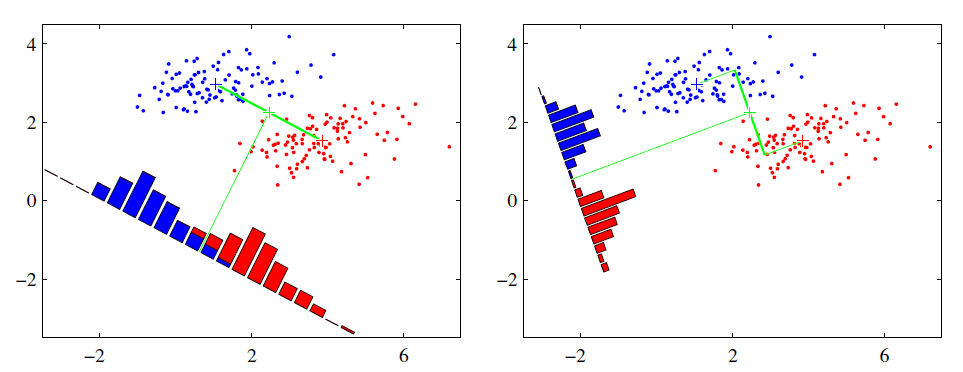
\includegraphics[width=0.55\textwidth]{lda-bi}
  \caption{二类LDA转换效果图 \label{fig:lda-bi}}
\end{figure}

假定数据集$D=\{(x_1, y_1), (x_2, y_2), ..., (x_m, y_m)\}$,其中$x_i \in R^{n}$,$y_i \in \{0, 1\}$。我们定义$N_j (j=0,1)$为第$j$类样本的个数,$X_j (j=0,1)$为第$j$类样本的合集,$\mu_j (i=0,1)$为第$j$类样本的均值向量,$\Sigma_j (j=0,1)$为第$j$类样本缺少分母部分的协方差矩阵。那么$\mu_j$和$\Sigma_j$的表达式分别如公式\ref{eqn:lda-mean}和公式\ref{eqn:lda-var}所示。
\begin{align}
\mu_j &= \frac{1}{N_j} \sum_{x\in{j}} x  \label{eqn:lda-mean}\\
\Sigma_j &= \sum_{x\in{j}} (x-\mu_{j})(x-\mu_{j})^{T} \label{eqn:lda-var}
\end{align}

由于只有两类数据,所以只需要将这些数据投影到一条直线上就可以,假设投影向量为$w$,则对任意一个样本,其在直线上的投影为$w^{T}x$,类别中心的投影分别为$w^{T}\mu_{0}$和$w^{T}\mu_{1}$,LDA要求不同类别之间的类别中心尽可能的远,所以需要最大化$\parallel w^{T}\mu_{0} - w^{T}\mu_{1} \parallel_{2}^{2}$,同时我们还希望同一类别尽可能接近,也就是样本投影之后的协方差尽可能的小,投影后的协方差如公式\ref{eqn:shadow-var}。
\begin{align}
\label{eqn:shadow-var}
\begin{split}
\Sigma_{j}^{'} &= \sum_{x\in{j}} (w^{T}x-w^{T}\mu_{j})(w^{T}x-w^{T}\mu_{j})^{T} \\
               &= \sum_{x\in{j}} w^{T}(x-\mu_{j})(x-\mu_{j})^{T}w \\
               &= w^{T}\Sigma_{j} w
\end{split}
\end{align}
所以我们希望最小化 $w^{T}\Sigma_{0} w + w^{T}\Sigma_{1} w$,由此我们可以得到需要优化的目标函数,如公式\ref{eqn:lda-obj-bi}。
\begin{align}
\label{eqn:lda-obj-bi}
\begin{split}
\arg\mathop{\max}_{w} J(w) &= \arg\mathop{\max}_{w}  \frac{\parallel w^{T}\mu_{0} - w^{T}\mu_{1} \parallel_{2}^{2}}{w^{T}\Sigma_{0} w + w^{T}\Sigma_{1} w} \\
                           &= \arg\mathop{\max}_{w}  \frac{w^{T} (\mu_{0} - \mu_{1}) (\mu_{0} - \mu_{1})^{T}w }{w^{T}(\Sigma_{0} + \Sigma_{1}) w} \
\end{split}
\end{align}

类内散度矩阵$S_w$和类间散度矩阵$S_b$分别定义为公式\ref{eqn:intra-matrix}和公式\ref{eqn:inter-matrix}。
\begin{align}
S_w &= \Sigma_{0} + \Sigma_{1} \label{eqn:intra-matrix}\\
S_b &= (\mu_{0} - \mu_{1}) (\mu_{0} - \mu_{1})^{T}  \label{eqn:inter-matrix}
\end{align}

所以目标函数就变成了:
\begin{align}
\label{eqn:lda-obj-bi-rui}
\arg\mathop{\max}_{w} J(w)  &= \arg\mathop{\max}_{w} \frac{w^{T}S_{b}w}{w^{T}S_{w}w} 
\end{align}

也就是求解出$w$使得$J(w)$最大。根据\ref{sec:rayleigh-quotient}中的介绍,我们可以通过计算矩阵$S_{w}^{-1}S_{b}$的特征值和特征向量得到对应的$w$,即求解公式\ref{eqn:lda-di-solve}。$J(w)$的最大值为$S_{w}^{-1}S_{b}$的最大特征值,最小值为$S_{w}^{-1}S_{b}$的最小特征值,而$S_w$和$S_b$均可由原始数据求解得出,因此很容易就可以求解出$J(w)$的最大值。
\begin{align}
\label{eqn:lda-di-solve}
S_{w}^{-1}S_{b}w = \lambda{w}
\end{align}

接下来我们分析下多类LDA的原理。

假定数据集$D=\{(x_1, y_1), (x_2, y_2), ..., (x_m, y_m)\}$,其中$x_i \in R^{n}$,$y_i \in \{C_1, C_2, ..., C_k\}$。我们定义$N_j (j=0,1,...,k)$为第$j$类样本的个数,$X_j (j=0,1,...,k)$为第$j$类样本的合集,$\mu_j (i=0,1,...,k)$为第$j$类样本的均值向量,$\Sigma_j (j=0,1,...,k)$为第$j$类样本缺少分母部分的协方差矩阵。此时是多类分类,因此投影后的空间不再是一条直线,而是一个超平面。假设投影后的低维空间维度为$d$,对应的基向量为$(w_1, w_2,..., w_d)$,基向量组成的矩阵为$W\in{R^{n*d}}$。

此时类内的散度矩阵$S_W$仍旧存在,如公式\ref{eqn:intra-multi}。
\begin{align}
\label{eqn:intra-multi}
S_W = \sum_{j=1}^{k} \Sigma_{j} 
\end{align}

但是类间的散度矩阵就有所不同了。此时用每个类别的均值到全局均值的距离来衡量类间距如图\ref{fig:lda-mul}。
\begin{figure}[htbp]
  \centering
  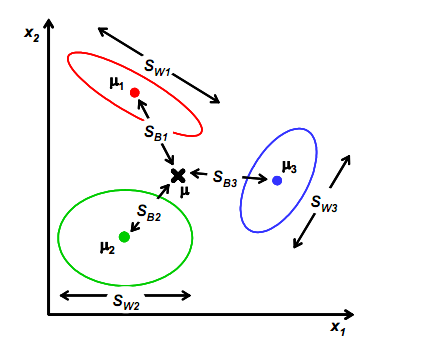
\includegraphics[width=0.55\textwidth]{lda-mul}
  \caption{多类LDA的类间散度矩阵示意图 \label{fig:lda-mul}}
\end{figure}

其定义为公式\ref{eqn:inter-multi}。
\begin{align}
\label{eqn:inter-multi}
S_B = \sum_{j=1}^{k} N_j (\mu_{j} - \mu)(\mu_{j} -\mu)^{T}
\end{align}
其中:
\begin{align}
\mu     &= \frac{1}{m}\sum_{i=1}^{m} x_{i} \\
\mu_{j} &= \frac{1}{N_{j}}\sum_{x_{j}\in{C_{j}}} x_{j}
\end{align}

同样此时的优化目标为公式\ref{eqn:lda-obj-multi}。
\begin{align}
\label{eqn:lda-obj-multi}
\arg\mathop{\max}_{W} J(W)  &= \arg\mathop{\max}_{W} \frac{W^{T}S_{B}W}{W^{T}S_{W}W} 
\end{align}

此时目标函数求解转换成了公式\ref{eqn:lda-mul-solve}:
\begin{align}
\label{eqn:lda-mul-solve}
S_{W}^{-1}S_{B}W = \lambda{W}
\end{align}

以上,可以总结出多类LDA的求解步骤:
\begin{enumerate}
  \item 计算每个类别的均值向量和方差,以及全局均值向量;
  \item 根据均值向量和方差,计算$S_w$和$S_B$;
  \item 对$S_{W}^{-1}S_{B}W = \lambda{W}$进行求解,求出$S_{W}^{-1}S_{B}$的特征值和特征向量;
  \item 对特征向量进行排序,设定低维空间的维度$d$,选取前$d$个特征值和特征向量,特征向量组合成投影矩阵$W$;
  \item 通过投影矩阵计算出投影后的输入数据$x_{i}^{'}=W^{T}x_{i}$;
  \item 得到输出的新数据集:$\{(x_{1}^{'}, y_1), (x_{2}^{'}, y_2), ..., (x_{m}^{'}, y_m)\}$。
\end{enumerate}

%------------------------------------------------------------------------------
%                                       MLLT
%------------------------------------------------------------------------------
\section{最大似然线性变换}
最大似然线性变换(Maximum Likelihood Linear Transform)

在HMM系统中,协方差矩阵的选择可以是对角阵,分块对角阵或者全矩阵。相对于对角阵来说,全矩阵的优势在于对特征向量元素之间关系的建模,劣势在于参数量巨大。

%------------------------------------------------------------------------------
%                                       Beta
%------------------------------------------------------------------------------
\section{Beta分布}
  
%------------------------------------------------------------------------------
%                                   MLE vs MAP
%------------------------------------------------------------------------------
\section{MLE和MAP}

\href{https://wiseodd.github.io/techblog/2017/01/01/mle-vs-map/}{MLE vs MAP}

\section{熵相关}


\chapter{微软Edx语音识别笔记}
本章笔记主要是对微软Edx的课程\href{https://courses.edx.org/courses/course-v1:Microsoft+DEV287x+1T2019a/course/}{Speech Recognition System}的记录,首版主要是翻译,再加上自己翻阅其他资料综合起来的一些思考和总结。代码见\href{https://github.com/MicrosoftLearning/Speech-Recognition}{Speech-Recognition}

%------------------------------------------------------------------------------
%                                Fundamentals
%------------------------------------------------------------------------------
\section{Background and Fundamentals}
\subsection{Phonetics} % (fold)
\label{ssub:phonetics}
Phonetics(语音学)是Linguistics(语言学)的一个分支,其研究的是人类语音发出的声音(sound)。语音学围绕着声音的产生(通过人类的发音器官)、声音的声学特性和感知。语音学有三个基本的分支,这三个分支都与ASR有关系。
\begin{enumerate}
	\item Articulatory Phonetics(发音语音学):通过发音器官、不同说话人而产生的声音;
	\item Acoustic Phonetics(声学语音学):声音从说话人到听者的传输;
	\item Auditory Phonetics(听觉语音学):听者对于声音的接收和感知。
\end{enumerate}

声音的最小单元我们成为\textcolor{red}{Phoneme},即音素。序列中的词(Words)是由一个或多个音素组成的。一个音素的声学实现称为\textcolor{red}{Phone}。图\ref{fig:exam-phonemes}展示了美式英语的音素和一般实现办法。
\begin{figure}[htbp]
  \centering
  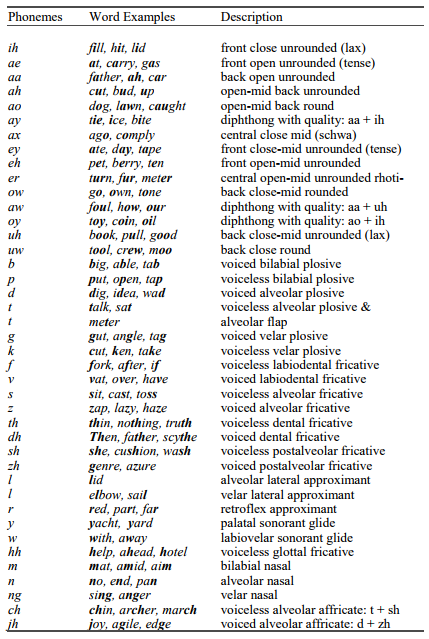
\includegraphics[width=0.35\textwidth]{phonemes}
  \caption{美式英语的音素和一般实现办法 \label{fig:exam-phonemes}}
\end{figure}

一般我们将音素分为两类:元音(Vowel)和辅音(Consonants)。
\begin{enumerate}
	\item Vowels:元音有两个特点,一是元音都是发声的声音(voiced sound),这意味着从声带(vocal chords)到口腔(mouth cavity)的气流是由声带的某种基频的震动(或者音高)产生的。二是舌头在生产过程中不会以任何方式形成气流收缩。每个元音发声的时候舌头、嘴唇和下巴的造型都不一样。这些不同的方式形成了不同的共振态,我们称之为共振峰。这些共振峰的共振态频率形成了不同的元音。
	\item Consonants:辅音是通过在口腔中或者空气中很明显的气流收缩形成的。有些辅音和元音一样是发声的,有些是不发声的。不发声的音素不会激活声带,因此也不存在基频或者音高。一些辅音音调成对出现,只有在有声或无声的情况下才有所不同,但在其他方面是相同的。比如说/b/和/p/这两个音素的发音方式是相同的,因为你的嘴唇、下巴还有舌头的姿势是一样的。但是/b/是发声的,/p/是不发声的。
\end{enumerate}

音素的另外一个重要特性是\textcolor{red}{其根据不同的上下文音素发音是会改变的}。我们称之为Phonetic Context。之所以会这样,是因为协同发音(coarticulation)。这些声音连续起来发音会改变其原有的特征。由协同发音产生的音素我们称为音素变体(allophones)。

所有当前的这些语音识别系统都使用了音素的语境相关的特性来建立处于不同phonetic context的音素模型。
% subsubsection phonetics (end)

\subsection{Words and Syntax} % (fold)
\label{sub:words_and_syntax}
Syllable 是一串声音,是个序列,由一个核心的音素,可能有初始音素和终止音素,这个核心音素一般是个元音或者一个音节辅音(syllablic consonant),是能够唱出来或者吼出来的声音。

举个例子,英文单词 "bottle" 包含两个 syllable 。第一个 syllable 有三个 phone ,在 Arpabet 音素描述代码里,是 "b aa t" 。这个 "aa" 就是核心音素,"b" 是发声的初始音素,"t" 是不发音的终止音素;第二个 syllable 是只包含一个 syllablic cosonant "l"。

一个 syllable 也可以组成一个词,其本身就是一个单独的音素,比如说,"Eye","uh",或者"eau"(医:水)。

语音识别里面,syllable 很少会考虑作为声学模型的建模单元,而词一般是变成音素来建模。

Syntax(句法规则)描述了给定词和定义了语法的规则下,句子的形成。而 Semantics(语义学)一般指代的是句子中的词或者短语是如何形成句意的。Syntax 和 Semantics 是 NLP 的重要组成部分,但是在语音识别里面,不起主要作用。
% subsection words_and_syntax (end)

\subsection{Measuring Performance} % (fold)
\label{sub:measuring_performance}
在语音识别系统的搭建和实验中,如何来衡量一个系统的好坏呢?由于语音识别是一个序列任务,跟图像当中的分类不一样,因此我们在衡量系统的性能时需要考虑到整个序列。

语音识别准确率衡量最常用的一个指标是词错误率(word error rate,WER)。一般识别出来的结果可能会产生三种错误:替换(substitution)、删除(delete)和插入(insert)。替换指的是一个词被识别成了另外一个词;删除指的是原本有词,但是没有识别出来;插入指的是原本没有词,多识别出来了词。WER 的计算方式如公式\ref{eqn:wer}。
\begin{align}
\label{eqn:wer}
  WER = \frac{N_{sub}+N_{ins}+N_{del}}{N_{ref}}
\end{align}
其中$N_{sub}$、$N_{ins}$和$N_{del}$分别是替换、插入和删除的数量,而$N_{ref}$是参考文本描述中词的个数。

WER的计算用的是通过计算实际输出描述和参考文本描述之间的\href{https://en.wikipedia.org/wiki/Edit_distance}{字符串编辑距离}得到的。编辑距离的实现通过动态规划算法。因为长文本的编辑距离可能不可靠,所以我们通过逐句的计算累积的错误,这些错误最终整合到一起来计算测试集的WER。

表\ref{tab:wer}呈现了实际输出和参考文献之间的不同,以及对应的三种错误。
\begin{lstlisting}[language = python, numbers=left, 
         numberstyle=\tiny,keywordstyle=\color{blue!70},
         commentstyle=\color{red!50!green!50!blue!50},frame=shadowbox,
         rulesepcolor=\color{red!20!green!20!blue!20},basicstyle=\ttfamily]
Ref: however a little later we had a comfortable chat
Hyp: how never a little later he had comfortable chat
\end{lstlisting}
\begin{table}[h]
 \centering
 \caption{WER计算公式中的三种错误实例演示}
   \begin{tabular*}{1\textwidth}{@{\extracolsep{\fill}}ccc}
   \toprule
    {\bf Reference} & {\bf Hypothesis} & {\bf Error} \\
   \midrule
   however      &        how  & Substitution \\ \hline
                &      never  &  Insertion   \\ \hline
         a      &          a  &              \\ \hline
    little      &     little  &              \\ \hline
    later       &      later  &              \\ \hline
    we          &         he  & Substitution  \\ \hline
    had         &        had  &              \\ \hline
    a           &             &   Deletion   \\ \hline
	comfortable   & comfortable &              \\ \hline
      chat      &       chat  &              \\
   \bottomrule
   \end{tabular*}%
 \label{tab:wer}%
\end{table}%

在某些情况中,这三种错误的成本不对等,那么计算编辑距离的时候可以作相应的调整。

句错误率(Sentence Error Rate,SER)是另外一种衡量系统的标准,其计算方式是整句没有出现任何错误。SER 仅仅作为一个指标,来看下错误的句子占全部句子的比例。

% subsection measuring_performance (end)

\subsection{Significance Testing} % (fold)
\label{sub:significance_testing}
统计显著性检验(statistical significance testing)涉及测量两个实验(或算法)之间的差异在多大程度上归因于两个算法中的实际差异,或者仅仅是数据,实验设置或其他因素中的结果固有变异性。统计显著性是所有分类任务的基石,只是统计显著性检验的方法取决于任务的特性。大多数方法的核心是假设检验的概念中存在一个无效假设。问题在于你有多大的confidence能够说无效假设会被拒绝。

对于语音识别来说,比较两个实验或者算法最常用的方法是 Matched Pairs Sentence-Segment Word Error(MAPSSWE)检验,简称为 Matched Pairs Test\upcite{asr-sign}。

在这个方法中,测试集被分为几份,假设这些子测试集中任意一个的错误都与其他子测试集统计独立。这个假设和语音识别的实验很贴合,因为测试数据都是一句一句的经由识别器输出结果。给定了每一个句子的WER,就很容易构建一个matched pairs\upcite{Pallet1990Tools}。
% subsection significance_testing (end)

\subsection{Other Consideration} % (fold)
\label{sub:other_consideration}
除去准确率,对识别系统性能的影响还可能包括计算需求,处理速度或者延迟什么的。解码速度一般用实时因子(real-time factor,RTF)来衡量。RTF为1.0指的是系统处理10s的数据需要花10s的时间。

RTF高于1.0意味着系统要花更多的时间来解码,对于某些应用,也许是可以接受的,比如希望获得一个会议或者讲座的转写,相对于快速的得到转写结果,准确率可能更重要一些,因此多花一些时间也是可以接受的。

当RTF低于1.0,系统会在当前数据达到前就处理好了之前的数据。当不止一个系统在同一个机器上运行的时候,这个就比较有用了。在这种情况下,我们可以用多线程来并行处理多路音频流。此外RTF低于1.0意味着系统能够满足在线实时解码的音频流应用。比如说,当我们在处理一个手机上远程音频需求的时候,网络阻塞可能会使得服务器接收音频产生间隙和延迟。如果语音识别器能够以比实时更快的速度来处理,那么它就可以在数据达到之后迅速跟进,追上最新的音频进度,以速度来掩盖网络的延迟。

一般来说,语音识别系统能够在准确率和速度之间调整,但是这种调整也是有限的,不可能无限好或者无限快。对于一个给定的模型和测试集,speed-accuracy图有一条不可被突破的渐近线(asymptote),即便给予无限的算力。所以准确率是有个极限的,这个时候的错误率可以认为就是模型带来的错误。一旦根据模型搜索找到了最好的结果,进一步的处理也不会带来准确率上的提升。
% subsection other_consideration (end)

\subsection{The Fundamental Equation} % (fold)
\label{sub:the_fundamental_equation}
语音识别可以看作一个优化任务。特别地,给定一个观测序列$O=\{O_{1},...,O_{N}\}$,我们找寻的是最有可能的词序列$W=\{W_1,...,W_M\}$,也就是说我们要找到最大化后验概率$P(W|O)$的词序列,如公式\ref{eqn:fundamental-equation}。
\begin{align}
\label{eqn:fundamental-equation}
  \hat{W} = \arg\mathop{\max}_{W} P(W|O)
\end{align}
利用贝叶斯规则,我们得到公式\ref{eqn:fun-bayes}。
\begin{align}
\label{eqn:fun-bayes}
  P(W|O) = \frac{P(W)P(O|W)}{P(O)}
\end{align}

因为词序列并不依赖于观测序列的边缘概率分布$P(O)$,我们可以忽略这个部分,综合上述两个公式,我们得到公式\ref{eqn:fun-final}。
\begin{align}
\label{eqn:fun-final}
  \hat{W} = \arg\mathop{\max}_{W} P(W)P(O|W)
\end{align}

这就是语音识别的基本公式。语音识别问题就可以看作是在这个联合模型上的搜索。

公式中的$P(O|W)$叫做\textcolor{red}{声学模型(acoustic model)}。这个模型描述了在给定词序列$W$的条件下,声学观测$O$的分布。声学模型表征的是词序列是如何转换成声学实现的,进而转换成ASR系统的声学观测的。

公式中的$P(W)$叫做\textcolor{red}{语言模型(language model)},其只取决于词序列$W$。语言模型给每一个可能的词序列一个概率值。它是由日常使用的一些词序列训练成的。一个训练好的英语语言模型会给"I like turtles"高的概率值,给"Turtles sing table"低的概率值。语言模型促使着词序列的搜索沿着训练数据中的模式开展。语言模型也可以在一些纯文本的应用中见到,比如浏览器的自动补全等。

由于诸多原因,构建一个语音识别系统比这个简单地公式所能呈现的要复杂的多得多。
% subsection the_fundamental_equation (end)
\subsection{Lab 1: Create a speech recognition scoring program} % (fold)
\label{sub:lab-1}
本模块有一个实验作业,标题为"Create a speech recognition scoring program"。

{\bf Required files:}
\begin{itemize}
	\item \textcolor{blue}{wer.py}
	\item \textcolor{blue}{M1\_score.py}
\end{itemize}}

{\bf Instructions:}

In this lab, you will write a program in Python to compute the word error rate (WER) and sentence error rate (SER) for a test corpus. A set of hypothesized transcriptions from a speech recognition system and a set of reference transcriptions with the correct word sequences will be provided for you.

This lab assumes the transcriptions are in a format called the "trn" format, created by NIST. The format is as follows. The transcription is output on a single line followed by a single space and then the root name of the file, without any extension, in parentheses. For example, the audio file "tongue\_twister.wav" would have a transcription

sally sells seashells by the seashore (tongue\_twister)

Notice that the transcription does not have any punctuation or capitalization, nor any other formatting (e.g. converting "doctor" to "dr.", or "eight" to "8"). This formatting is called "Inverse Text Normalization" and is not part of this course.

The python code \textcolor{blue}{M1\_Score.py} and \textcolor{blue}{wer.py} contain the scaffolding for the first lab. A main function parses the command line arguments and string\_edit\_distance() computes the string edit distance between two strings.

Add code to read the trn files for the hypothesis and reference transcriptions, to compute the edit distance on each, and to aggregate the error counts. Your code should report:
\begin{itemize}
	\item Total number of reference sentences in the test set
	\item Number of sentences with an error
	\item Sentence error rate as a percentage
	\item Total number of reference words
	\item Total number of word errors
	\item Total number of word substitutions, insertions, and deletions
	\item The percentage of total errors (WER) and percentage of substitutions, insertions, and deletions
\end{itemize}

The specific format for outputting this information is up to you. Note that you should not assume that the order of sentences in the reference and hypothesis trn files is consistent. You should use the utterance name as the key between the two transcriptions.

When you believe your code is working, use it to process hyp.trn and ref.trn in the misc directory, and compare your answers to the solution.
% subsection lab (end)

%------------------------------------------------------------------------------
%                                Speech Signal Processing
%------------------------------------------------------------------------------
\section{Speech Signal Processing}
\subsection{Introduction} % (fold)
\label{sub:introduction}
通过空气传播的音频波形通过麦克风的捕捉,将这些压力波转换成可捕捉的电信号活动。对这些电信号活动进行采样,这样就得到了一系列采样波形,我们用这些波形来描述信号。音乐信号一般采样率为 44100 Hz,即一秒钟会有44100个采样点。根据奈奎斯特定理(Nyquist theorem),只有频率低于22050 Hz的音频才可以被捕捉到。如果信号的高频部分比较少,最高频率为8000Hz的话,采样率一般就是16000Hz。传统的电话和大部分的手机带限是3400 Hz,所以8000 Hz的采样率就足够了。所以电话语音的采样率一般就是 8000Hz。

一个典型的音频波形图如\ref{fig:wavform}(左),其说的句子是"speech recognition is cool stuff"。
\begin{figure}[!ht]
  \centering
  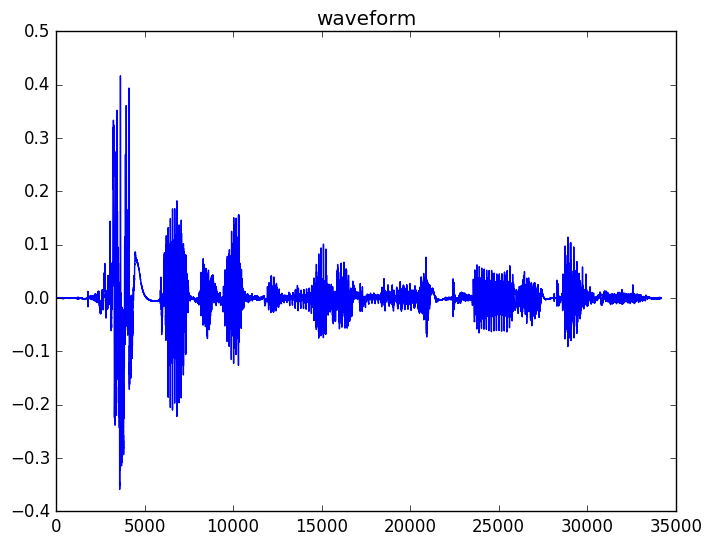
\includegraphics[width=0.45\textwidth]{waveform}
  \hspace{1cm}
  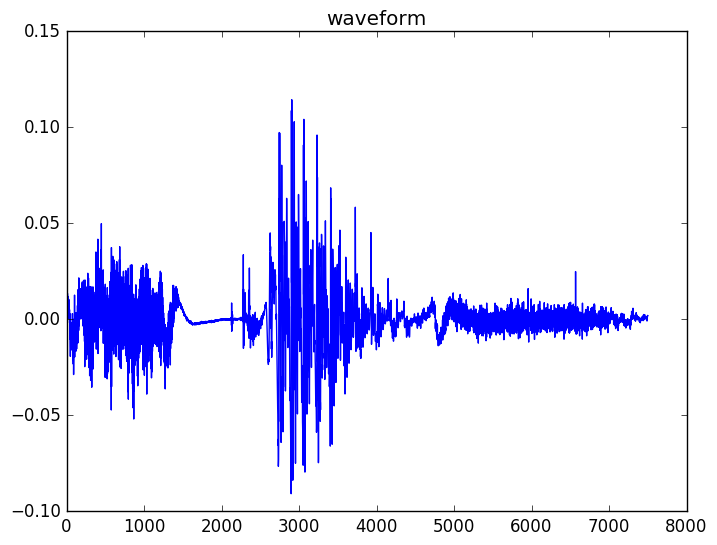
\includegraphics[width=0.45\textwidth]{stuff}
  \hspace{1cm}
  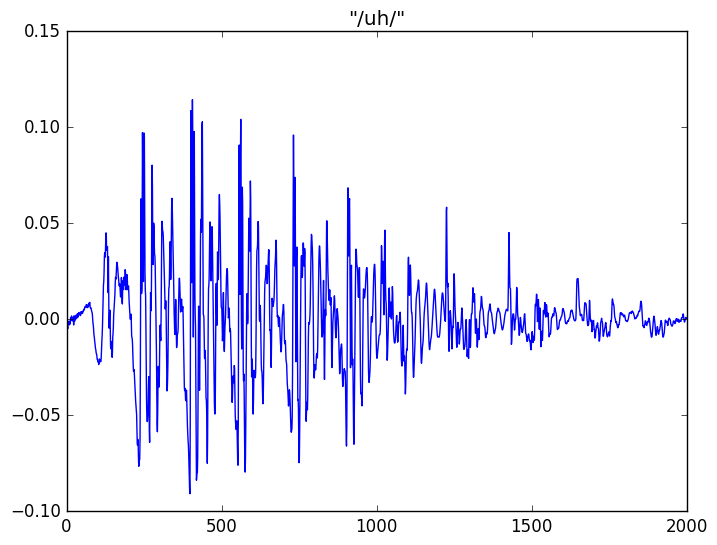
\includegraphics[width=0.45\textwidth]{uh}
  \caption{完整音频波形图与部分波形图}
\label{fig:wavform}
\end{figure}

回忆上一节中讨论的发声音素和不发声音素,我们来瞅一下最后一个单词 "stuff" 的波形图,如图\ref{fig:wavform}(右)。从图上我们看到,这个单词的发音有三个不同的部分,初始不发声语音"st",中间发声语音"uh",终止不发声语音"f"。不发声的语音部分看上去像噪音,具有随机性。而发声部分的语音由于声带的振动而具有周期性。

在拉近一点,我们看看发声的这个元音"/uh/",如图\ref{fig:wavform}(下)可以更明显的看到这个元音的周期性。

从这些波形图中,我们可以看到波形的特征形成有两方面的因素:(1)声带的应激反应(excitation)趋势着空气从声道和嘴巴流出;(2)发出某种特定声音时,声道本身的形状。

举例来说,图\ref{fig:wavform}(右)中"st"和"f"看上去都像噪声,但是他们的形状却不相同,就是因为他们是不一样的声音。而"uh"的声音更具周期性,因为发声的应激反应,其由于发声的时候声道的作用有独特的形状。所以对于同一个说话人来说,不同的元音可能会有着相近的周期,但是波形的整体形状是不一样的,就因为这些波形都是由相同的声带产生的,但是发不同的声音声道是不一样的。

在信号处理中,一般用源滤波器模型(source-filter model)来对这个语音产生的过程进行建模。声源是由通过声道的声带产生的激励信号,我们将其建模成为时变线性滤波器。源滤波器在语音识别中有很多应用,比如语义分析和编码。而且有很多种办法来评估源信号和滤波器的参数,比如很有名的线性预测编码(Linear Predictive Coding,LPC)。

对于语音识别来说,音素分类在很大程度上取决于声道的形状,也就是说取决于源滤波器模型的滤波器部分。激励信号或者原信号大都被忽略或者舍弃了。所以语音识别的特征提取过程一般设计成捕捉话语过程的时变滤波器形状。
% subsection introduction (end)

\subsection{Feature Extraction} % (fold)
\label{sub:feature_extraction}
从波形图中,很明显语音是非平稳信号(non-stationary signal),这就意味着语音信号的统计特性会随着时间变化而变化。所以为了分析语音信号,我们需要将信号分成一个又一个 chunk(也成为窗或者帧),这些chunk短到可以认为它们是平稳信号。这样我们就可以去分析一系列短时的有重叠的语音帧。在语音识别中,我们一般选窗长为 25ms,窗移位 10ms,也就是说一秒钟会被分成100帧。

因为我们是从一个长音频提取的chunk,所以对于每一个chunk的边缘,我们要进行一些处理。一般对每一帧数据加个窗函数,常用的是汉明窗(Hamming Windows),当然也有用其他窗函数的。定义$m$为某一帧的索引,$n$为采样点的索引,$L$是这一帧采样点的个数,$N$是采样中的偏移量。那么从原始信号中提取出来的每一帧计算公式见\ref{eqn:frame-window}。
\begin{align}
\label{eqn:frame-window}
  x_{m}[n]=w[n] x[m N+n], n=0,1, \ldots, L-1
\end{align}
其中$w[n]$是窗函数。

然后我们利用离散傅里叶变换将每一帧的数据转换到频域,如公式\ref{eqn:fft}。所有现代软件中都可以有效的计算快速傅里叶变换。
\begin{align}
\label{eqn:fft}
  X_{m}[k]=\sum_{n=0}^{N-1} x_{m}[n] e^{-j 2 \pi k n N}
\end{align}

傅里叶表征$X_{M} [k]$是一个很复杂的数,因为它包含了每一帧和每一个频率的频谱幅值(绝对幅值)和相位信息。为了提取特征,我们去掉了相位信息,只考虑幅值 $|X_{m}[k]|$。

频谱图描述了对语音信号进行FFT操作得到的log幅值(或者log-power),如图\ref{fig:log-compare}(右)。横轴是帧索引(单位为10ms),纵轴是频率,其范围是0Hz到采样率的一般,也就是对应的Nyquist频率。图中呈现的是"speech recognition is cool stuff"。在频谱图中,黄色和红色区域表示该区域能量高。
% subsection feature_extraction (end)

\subsection{Mel Filtering} % (fold)
\label{sub:mel_filtering}
从频谱图中可以看出高频的高能量区域大致对应着不发声的辅音,低频的高能量区域大致对应着发声的元音。频谱图中,发声区域的水平线(horizonal lines)呈现的是语音的谐波结构(harmonic structure)。

由于发声区域的谐波结构和不发声区域的随机噪声,频谱中存在着变数(variability)。为了移除这些变数,我们对幅度谱(magnitude spectrum)进行频谱光滑操作。受听觉系统处理语音信号的启发,我们对频谱图进行滤波器组操作(filterbank),该滤波器组对频率轴进行了 approximately logarithmic scale。也就是说随着频率的升高,滤波器也会变得更宽间隔更大。最常用于特征提取的filterbank是 {\bf mel filterbank}。一个 mel filterbank 包含40个滤波器,如图\ref{fig:mel-fbank}。每一个滤波器会对不同频率区间的能量谱求平均。
\begin{figure}[htbp]
  \centering
  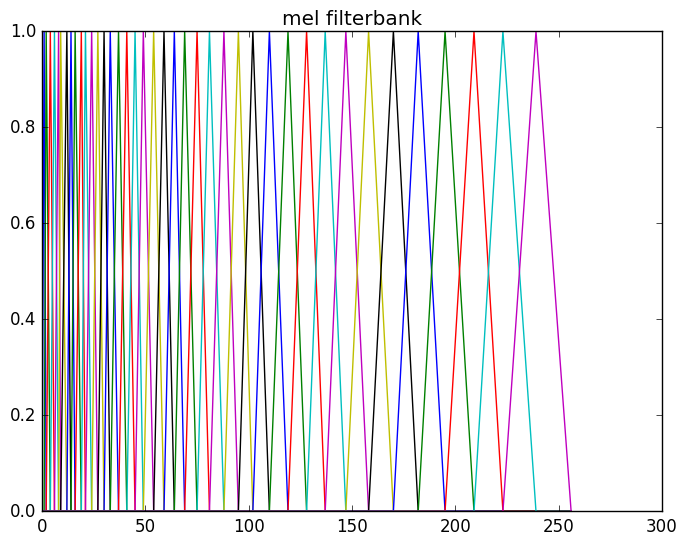
\includegraphics[width=0.45\textwidth]{mel-fbank}
  \caption{mel filterbank \label{fig:mel-fbank}}
\end{figure}

mel filterbank图在左边的滤波器很密集,在右边的滤波器间隔就比较远了。这是符合人耳听觉系统的,因为人耳对低频的信号更加敏感,对高频的信号不太敏感,所以低频的信息是更重要的,那么就需要多一些滤波器,从而提取更多有效特征。

P维的 mel filterbank的系数计算公式如\ref{eqn:mel-fbank}。一个 mel filterbank一般会计算出40个系数,虽然现代系统有的会多一些或者少一些。平滑过多,系数就少一些,反之则反之。
\begin{align}
\label{eqn:mel-fbank}
  X_{\mathrm{mel}}[p]=\sum_{k} M[p, k]\left|X_{m}[k]\right|, \quad p=0,1, \ldots, P-1
\end{align}

% subsection mel_filtering (end)

\subsection{Log Compression} % (fold)
\label{sub:log_compression}
特征提取的最后一步是对经过滤波器组得到的系数进行对数压缩。这个操作有助于压缩信号的动态范围,还能模拟听觉系统对声音的非线性压缩效果。我们把对数压缩后的输出称为 "filterbank" 系数。

将提取的特征以频谱图式的方式呈现出来之后,如图\ref{fig:log-compare}(左),与原始信号频谱图(右)进行比较,我们可以看出沿着频率轴的Fbank系数要平滑得多,这是因为高频噪声和pitch/谐波结构都被移除了。
\begin{figure}[!ht]
  \centering
  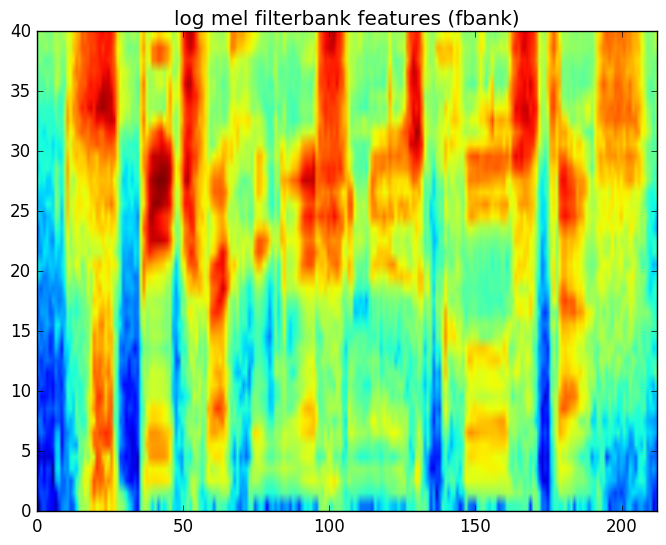
\includegraphics[width=0.45\textwidth]{figure/log-mel-fbank}
  \hspace{1cm}
  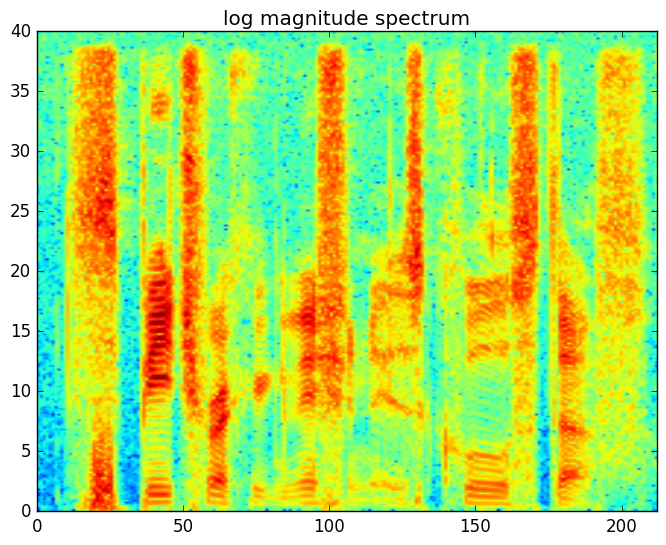
\includegraphics[width=0.45\textwidth]{figure/log-power}
  \caption{提取Fbank特征(左)与原始信号的频谱图(右)}
\label{fig:log-compare}
\end{figure}
% subsection log_compression (end)

除了上面的这些操作,在提取特征的过程中可能还会有一些其他的操作。其中有:
\begin{enumerate}
  \item Dithering(抖动):在原始音频信号中加入一个很小的噪声,为了防止在提取特征的时候出现数学问题,尤其是出现$\log0$;
  \item DC-removal(直流常数移除):在提取特征之前,去除音频中的常数偏置;
  \item Pre-emphasis(预加重):在提取特征之前用一个高通滤波器处理信号,因为发声的语音部分低频能量比不发声的语音部分高频能量要大得多,用一个高通滤波器来抵消下这个问题。实际操作的时候就是用了一个简单地线性滤波器,见公式\ref{eqn:pre-emp},其中$\alpha=0.97$。
    \begin{align}
    \label{eqn:pre-emp}
    y[n]=x[n]-\alpha x[n-1]
    \end{align}
  \item DCT(离散余弦变换):Fbank系数是强相关的,为了减弱这种相关性,将上述步骤提取出来的Fbank特征值再经过DCT。经过DCT之后的特征,一般取前13个,余下的由于所含信息不足舍弃了。DCT公式如\ref{eqn:dct}。
    \begin{align}
    \label{eqn:dct}
    d_t =\frac{\sum_{n=1}^{N}n(c_{t+n}-c_{t-n})}{2\sum_{n=1}^{N}n^2}
    \end{align}
\end{enumerate}}

\subsection{Feature Normalization} % (fold)
\label{sub:feature_normalization}
通信信道可能会对捕获的语音信号引入一些偏差(恒定滤波)。比如说,麦克风的频率响应不平稳,此外,即使相同语音的基础信号,其信号增益的变化也可能导致计算的滤波器组系数的差异。这些信道的影响可以用时域上的卷积进行建模,等价于频域表征的信号进行点乘(elementwise multiplication)。

因此信道的影响可以用恒定滤波来建模(constant filter),如公式\ref{eqn:model-channel}。
\begin{align}
\label{eqn:model-channel}
X_{t, \mathrm{obs}}[k]=H[k] X_{t}[k]
\end{align}
其观测幅度为:
\begin{align}
\label{eqn:ob-mag}
\left|X_{t, \mathrm{obs}}[k]\right|=|H[k]|\left|X_{t}[k]\right|
\end{align}

如果我们对公式\ref{eqn:ob-mag}两边取对数,并计算句子中所有帧的均值,则我们有公式\ref{eqn:log-mean}。
\begin{align}
\begin{split}
\label{eqn:log-mean}
\mu_{\mathrm{obs}}
    &=\frac{1}{T} \sum_{t} \log \left(\left|X_{t, \mathrm{obs}}[k]\right|\right) \\
    &=\frac{1}{T} \sum_{t} \log \left(|H[k]|\left|X_{t}[k]\right|\right) \\
    &=\frac{1}{T} \sum_{t} \log (|H[k]|)+\frac{1}{T} \sum_{t} \log \left(\left|X_{t}[k]\right|\right)\\
\end{split}
\end{align}

假设滤波器在时间轴上是常数,且语音信号的对数幅值均值为0,那么公式\ref{eqn:log-mean}可以简化为\ref{eqn:log-mean-simple}。
\begin{align}
\label{eqn:log-mean-simple}
  \mu_{t t o b s}=\log (|H[k]|)
\end{align}

以上,如果我们计算出句子的对数幅值的均值,并且对句子中的每一帧都减去这个均值,这样我们就可以除去信号中所有的恒定信道效应。

为了简便,我们直接对取了$\log$之后fbank特征进行归一化(normalization)。为了对比一系列操作的结构,图\ref{fig:fbank-normalization}展现了原始信号的频谱图(左)、fbank特征的频谱图(右)和对fbank特征归一化后的频谱图(下)。
\begin{figure}[!ht]
  \centering
  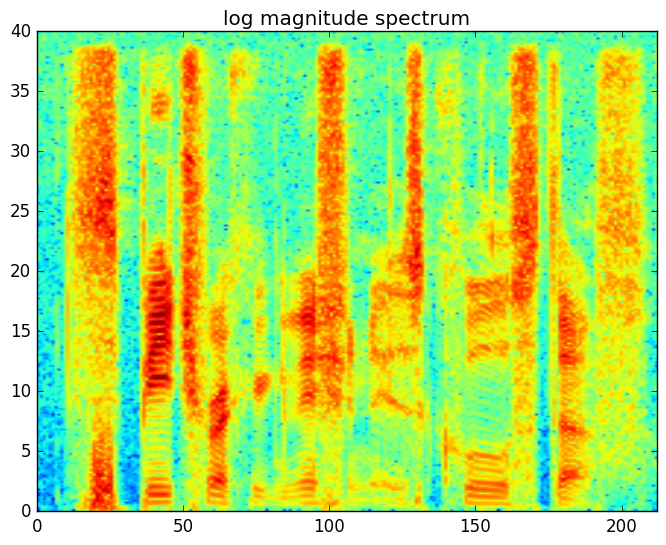
\includegraphics[width=0.40\textwidth]{figure/log-power}
  \hspace{0.5cm}
  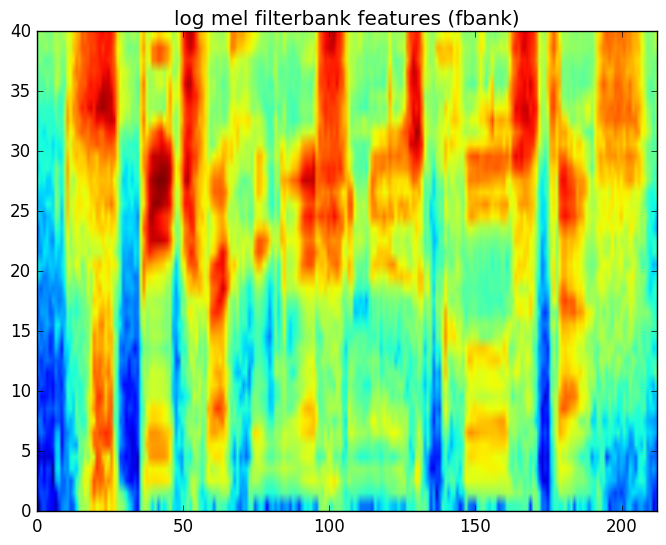
\includegraphics[width=0.40\textwidth]{figure/log-mel-fbank}
  \hspace{0.5cm}
  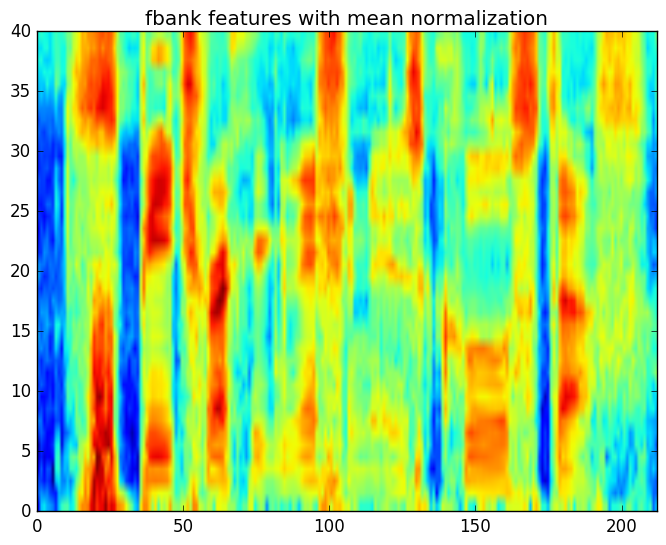
\includegraphics[width=0.40\textwidth]{figure/log-mel-fbank-norm}
  \caption{原始信号的频谱图(左)、提取Fbank特征(右)和归一化后的Fbank特征(下)}
\label{fig:fbank-normalization}
\end{figure}
% subsection feature_normalization (end)
\subsection{Summary}
为了从语音信号中提取语音识别所需的特征,我们希望提取到与声道形状有关的时变频谱信息,其由源滤波器模型中的一个滤波器建模,计算语句中的特征步骤如下:
\begin{enumerate}
  \item 预处理信号,包括预加重和dithering;
  \item 将信号切割成有重叠部分的帧,一般帧长为 25ms,帧移为 10ms;
  \item 对于每一帧:
      \begin{itemize}
        \item 用汉明窗处理信号;
        \item 使用FFT进行傅里叶变换;
        \item 计算频谱的幅值;
        \item 应用 mel filterbank;
        \item 进行对数操作;
      \end{itemize}
  \item 如果需要进行信道补偿,则对每一帧的fbank系数进行均值归一化。
\end{enumerate}}

\subsection{Lab 2: Feature extraction for speech recognition} % (fold)
\label{sub:lab_2}
本模块有一个实验作业,标题为"Feature extraction for speech recognition"。

{\bf Required files:}
\begin{itemize}
  \item \textcolor{blue}{M2\_Wav2Feat\_Single.py}
  \item \textcolor{blue}{M2\_Wav2Feat\_Batch.py}
  \item \textcolor{blue}{speech\_sigproc.py}
  \item \textcolor{blue}{htk\_featio.py}
\end{itemize}}

{\bf Instructions:}

In this lab, you will write the core functions necessary to perform feature extraction on audio waveforms. Your program will convert an audio file to a sequence of log mel frequency filterbank ("FBANK") coefficients.

The basic steps in features extraction are
\begin{enumerate}
  \item Pre-emphasis of the waveform
  \item Dividing the signal into overlapping segments or frames
  \item For each frame of audio:
    \begin{itemize}
      \item Windowing the frame
      \item Computing the magnitude spectrum of the frame
      \item Applying the mel filterbank to the spectrum to create mel filterbank coefficients
      \item Applying a logarithm operation to the mel filterbank coefficient
    \end{itemize}
\end{enumerate}
In the lab, you will be supplied with python file called {\bf speech\_sigproc.py}. This file contains a partially completed python class called {\bf FrontEnd} that performs feature extraction, using methods that perform the steps listed above. The methods for dividing the signal into frames (step 2) will be provided for you, as will the code for generating the coefficients of the mel filterbank that is used in step 3c. You are responsible for filling in the code in all the remaining methods.

There are two top-level python scripts that call this class. The first is called {\bf M2\_Wav2Feat\_Single.py}. This function reads a single pre-specified audio file, computes the features, and writes them to a feature file in HTK format.

In the first part of this lab, you are to complete the missing code in the {\bf FrontEnd} class and then modify {\bf M2\_Wav2Feat\_Single.py} to plot the following items:
\begin{enumerate}
  \item Waveform
  \item Mel frequency filterbank
  \item Log mel filterbank coefficients
\end{enumerate}

You can compare the figures to the figures below. Once the code is verified to be working, the feature extraction program should be used to create feature vector files for the training, development, and test sets. This will be done using {\bf M2\_Wav2Feat\_Batch.py}. This program takes a command line argument {\bf –-set} (or {\bf -s} ) which takes as an argument either {\bf train}, {\bf dev}, or {\bf test}. For example

{\bf \$ python M2\_Wav2Feat\_Batch.py –set train}

This program will use the code you write in the {\bf FrontEnd} class to compute feature extraction for all the files in the LibriSpeech corpus. You need to call this program 3 times, once each for train, dev, and test sets.

When the training set features are computed ({\bf –set train}) the code will also generate the global mean and precision (inverse standard deviation) of the features in the training set. These quantities will be stored in two ASCII files in the {\bf am} direction for use by CNTK during acoustic model training in the next module.

Here are the outputs you should get from plotting:
\begin{figure}[!ht]
  \centering
  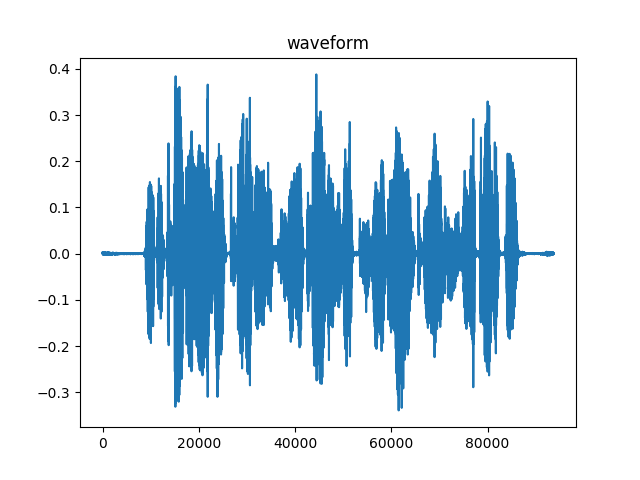
\includegraphics[width=0.30\textwidth]{figure/lab2-1}
  \hspace{0.5cm}
  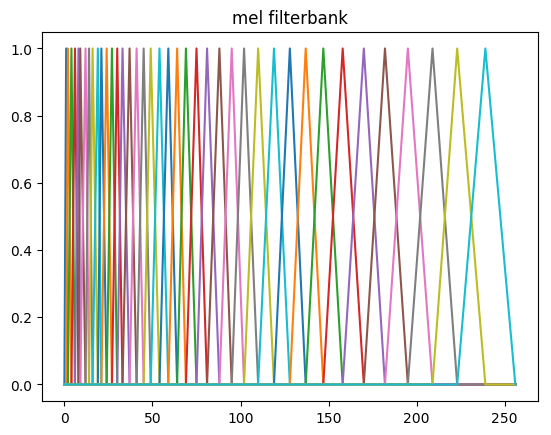
\includegraphics[width=0.30\textwidth]{figure/lab2-2}
  \hspace{0.5cm}
  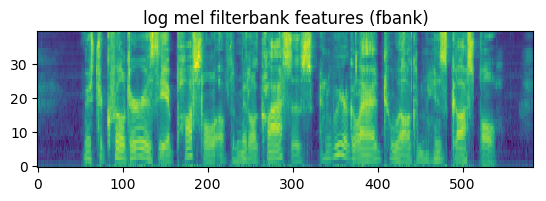
\includegraphics[width=0.30\textwidth]{figure/lab2-3}
  \caption{Lab 2的期望输出}
\label{fig:expect-output}
\end{figure}
% subsection lab_2 (end)

%------------------------------------------------------------------------------
%                                Acoustic Model
%------------------------------------------------------------------------------
\section{Acoustic Modeling}
\subsection{Introduction} 
本节讨论的是语音识别器中的声学模型。声学模型是一个混合模型,通过DNN得到逐帧的预测标签,再通过HMM将这些预测的音素转换成序列预测。HMM常用于对离散时间序列事件的建模。HMM的基本概念可以追溯到数十年前,而且HMM有很多应用。

\subsection{Markov Chains} 
了解一点马尔科夫链(Markov Chains)对学习HMM大有帮助。马尔科夫链是一种对随机过程进行建模的方法。在马尔科夫链中,用一系列状态(states)来对离散时间进行建模。状态之间的运动由随机过程控制。

举例说明,在一个天气预测的应用中,状态为 "{\bf S}unny"、"{\bf P}artly Cloud"、"{\bf C}loudy"、和"{\bf R}aining"。我们考虑某个连续五天的特定天气概率,比如$P(p,p,c,r,s)$,我们可以使用贝叶斯规则将这个联合概率分布打散成一系列条件概率的乘积,如公式\ref{eqn:markov1}。
\begin{align}
\label{eqn:markov1}
  p(X_1, X_2, X_3, X_4, X_5)=p(X_5 | X_4, X_3, X_2, X_1) p(X_4 | X_3, X_2, X_1) p(X_3 | X_2, X_1) p(X_2 | X_1) p(X_1)
\end{align}

假设天气模型满足一阶马尔科夫假设,即满足公式\ref{eqn:first-order}。
\begin{align}
\label{eqn:first-order}
  p(X_i |X_1, ..., X_{i-1})=p(X_i | X_{i-1})
\end{align}

那么连续五天天气的联合概率分布可以简化为公式\ref{eqn:markov2}。
\begin{align}
\label{eqn:markov2}
\begin{split}
  p(X_1, X_2, X_3, X_4, X_5)
      &= p(X_5 | X_4) p(X_4 | X_3) p(X_3 | X_2) p(X_2 | X_1) p(X_1) \\
      &= p(X_1)\prod_{i=2}^{5}p(x_i|x_{i-1})
\end{split}
\end{align}

一个马尔科夫链的核心元素有\textcolor{red}{状态的定义}(此处为天气预测)和\textcolor{red}{转移概率$p(X_i|X_{i-1})$},转移概率描述的是从一个状态移动到另一个状态的概率值(也包括转移到自身状态)。

比如说,天气预报的一个完整的(大体完整的)马尔科夫链可以用图\ref{fig:markov-weather}来表示。
\begin{figure}[htbp]
  \centering
  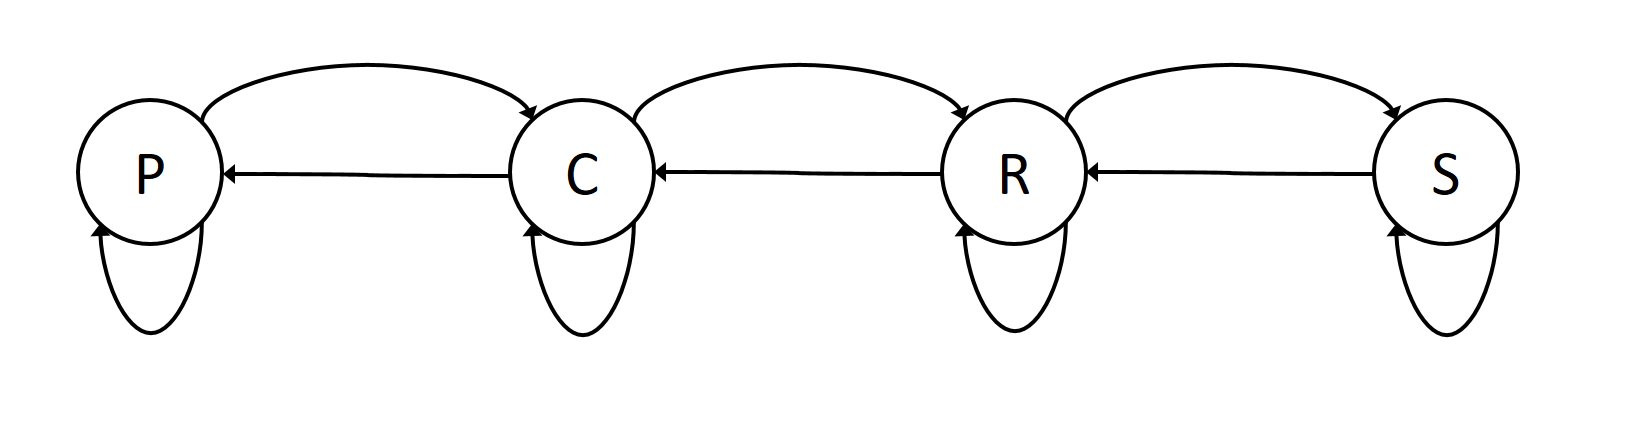
\includegraphics[width=0.45\textwidth]{markov-weather}
  \caption{天气预报模型的马尔科夫链\label{fig:markov-weather}}
\end{figure}

需要注意的是除了上面说的转移概率$p(X_i|X_{i-1})$,我们还需要知道这个序列的第一个元素,即第一天的某种天气的概率值$p(X_1)$。

所以除了状态清单和状态转移概率,我们还需要知道从马尔科夫链每一个状态开始的初始概率值。假设先验概率(每个状态的初始概率值)如公式\ref{eqn:markov-prior}。
\begin{align}
\label{eqn:markov-prior}
\begin{split}
  p(p) &= \pi_{p} \\
  p(c) &= \pi_{c} \\
  p(s) &= \pi_{s} \\
  p(r) &= \pi_{r}
\end{split}
\end{align}

现在我们回到这个例子,公式\ref{eqn:markov-weather-solu}说明了如何求$P(p,p,c,r,s)$。
\begin{align}
\label{eqn:markov-weather-solu}
\begin{split}
  p(p,p,c,r,s) &= p(s|p,p,c,r)p(r|p,p,c)p(c|p,p)p(p|p)p(p) \\
               &= p(s|r) p(r|c) p(c|p) p(p|p) p(p)
\end{split}
\end{align}

\subsection{Problems with Markov Models} 

\subsection{Hidden Markov Models} 

\subsection{Deep Neural Network Acoustic Models} 

\subsection{Training Feedforward Deep Neural Networks} 

\subsection{Using a Sequence based Objective Function} 

\subsection{Lab 3}

%------------------------------------------------------------------------------
%                                Language Modeling
%------------------------------------------------------------------------------
\section{Language Modeling}
\subsection{Introduction} 

\subsection{N gram Models}

\subsection{Language Model Evalution}

\subsection{Operations on Language Models}

\subsection{Advanced LM Topics}

\subsection{Lab 4}

%------------------------------------------------------------------------------
%                                Speech Decoding
%------------------------------------------------------------------------------
\section{Speech Decoding}
\subsection{Overview}

\subsection{Weighted Finite State Transducers}

\subsection{WFSTs and Acceptors}

\subsection{Graph Composition}

\subsection{Lab 5}


%------------------------------------------------------------------------------
%                                Advanced Acoustic Modeling
%------------------------------------------------------------------------------
\section{Advanced Acoustic Modeling}
\subsection{Imporved Objective Functions}

\subsection{Sequential Objective Function}

\subsection{Connectionist Temporal Classsification}

\subsection{Sequence Discriminative Objective Functions}

\subsection{Lab 6}


\section{补充知识点}

\subsection{傅里叶变换}

\subsection{Nyquist定理}
\chapter{Kaldi学习笔记}
\section{kaldi中的数据扰动}
kaldi程序中对原始数据进行扰动以达到数据增强的效果,一般是在单音素对齐,三音素对齐之后,在生成ivector的时候进行扰动处理,扰动有两种方式:速度扰动和音量扰动。如果存在segment文件的话,那么对应的起始和终止时间点会存在segment文件中,提取特征时会根据这个segment中存储的时间节点进行操作;如果不存在的话,相当于整段wav音频都是有效的,那么起始时间点和wav文件相同。扰动也会根据segment文件的有无进行对应的操作。

\subsection{速度扰动}

速度扰动一般是对音频进行加速和减速,根据Povey大佬的论文\href{https://www.danielpovey.com/files/2015_interspeech_augmentation.pdf}{《Audio Augmentation for Speech Recognition》}中的第二部分Audio Perturbation,对mel频谱进行一个偏移就能得到类似加速和减速的效果。首先定义一个扰动因子$\alpha$,假定segment中某一段音频的起始时间和终止时间为$t_1$和$t_2$,那么新的音频起始时间和终止时间计算方式如公式\ref{eqn:sp}。
\begin{align}
\label{eqn:sp}
\begin{split}
  t_{1}' = \frac{t_1}{\alpha} \\
  t_{2}' = \frac{t_2}{\alpha}
\end{split}
\end{align}

kaldi一般取$\alpha$为$0.9$和$1.1$以达到加速和减速的目的。得到了segment文件之后,在wav.scp文件中存储原始音频的位置,加速后音频sox指令和减速后音频sox指令。其详细的脚本指令见代码 utils/data/perturb\_data\_dir\_speed.sh 第74行。最终重新提取特征存于代码根目录下mfcc\_pertubed文件夹中。由于速度扰动对音频时间轴有改动,因此此时需要对音频进行重新对齐的操作。

\subsection{音量扰动}
音量扰动一般是对音频进行增大音量和减小音量。音量增加或者减小的幅度默认取$[0.125, 2]$之间的正态分布值。使用sox工具中的"sox - -vol #volume"来进行实际操作。其详细的脚本指令见代码 utils/data/perturb\_data\_dir\_volume.sh 第71行,其sox操作见代码 utils/data/internal/perturb\_volume.py。其重新提取的特征位于代码根目录下mfcc\_hires 文件夹中。此时由于仅仅对音频进行音量大小的扰动,并没有对时间维度进行操作,因此无需再进行一遍对齐操作,其标签对齐直接采用上一步即速度扰动后生成的对齐结果。此时重新提取特征时,MFCC特征的维度是40d。其原因是40d的MFCC和40d的Fbank维度相同,保存的信息量相似,同时MFCC由于其相关性较弱(DCT去相关),所以能更好的压缩特征,因此Kaldi一般都是采用40d的MFCC作为神经网络的输入特征(见kaldi的各个egs里conf下mfcc\_hires.conf)。
\begin{quotation}
"Config for high-resolution MFCC features, intended for neural network training. Note: we keep all cepstra, so it has the same info as filterbank features, but MFCC is more easily compressible (because less correlated) which is why we prefer this method. "
\end{quotation}

\section{kaldi中的UBM}

\href{http://citeseerx.ist.psu.edu/viewdoc/download?doi=10.1.1.117.338&rep=rep1&type=pdf}{通用背景模型UBM}(Universal Background Model)

\section{kaldi通过lattice输出语音对齐音素和词}

我们通过解码之后得到一堆的 lat.*.gz 文件,这些文件是lattice对齐后生成的对齐文件,其为压缩格式,所以首先通过 gunzip 指令对齐解压,我们以 lat.1.gz 为例来讲这一节的知识点。
\chapter{C++学习笔记}
\begin{lstlisting}[language=shell, numbers=left, 
         numberstyle=\tiny,keywordstyle=\color{blue!70},
         commentstyle=\color{red!50!green!50!blue!50},frame=shadowbox,
         rulesepcolor=\color{red!20!green!20!blue!20},basicstyle=\ttfamily]
gunzip exp/chain/tdnn7q_sp_online/decode_data_tgsmall/lat.1.gz
\end{lstlisting}

这样会在 exp/chain/tdnn7q_sp_online/decode_data_tgsmall/ 下生成一个 lat.1 文件,原先的 lat.1.gz 消失不见了…… lat.1 文件是二进制的格式,其由指令 online2-wav-nnet3-latgen-fatser 生成。
\chapter{FFmpeg和sox}
\section{FFmpeg}
\subsection{安装FFmpeg}
\href{https://www.jianshu.com/p/2b98e0f87720}{在Centos中利用yum安装FFmpeg}步骤如下:
\begin{enumerate}
\item 升级系统
\begin{lstlisting}[language = shell, numbers=left, 
         numberstyle=\tiny,keywordstyle=\color{blue!70},
         commentstyle=\color{red!50!green!50!blue!50},frame=shadowbox,
         rulesepcolor=\color{red!20!green!20!blue!20},basicstyle=\ttfamily]
sudo yum install epel-release -y
sudo yum update -y
sudo shutdown -r now
\end{lstlisting}
\item 安装Nux Dextop Yum源 \\
	由于CentOS没有官方FFmpeg rpm软件包。但是,我们可以使用第三方YUM源(Nux Dextop)完成此工作。
	\begin{itemize}
		\item CentOs 7
\begin{lstlisting}[language = shell, numbers=left, 
         numberstyle=\tiny,keywordstyle=\color{blue!70},
         commentstyle=\color{red!50!green!50!blue!50},frame=shadowbox,
         rulesepcolor=\color{red!20!green!20!blue!20},basicstyle=\ttfamily]
sudo rpm --import http://li.nux.ro/download/nux/RPM-GPG-KEY-nux.ro
sudo rpm -Uvh http://li.nux.ro/download/nux/dextop/el7/x86_64/nux-dextop-release-0-5.el7.nux.noarch.rpm
\end{lstlisting}
		\item CentOs 6
\begin{lstlisting}[language = shell, numbers=left, 
         numberstyle=\tiny,keywordstyle=\color{blue!70},
         commentstyle=\color{red!50!green!50!blue!50},frame=shadowbox,
         rulesepcolor=\color{red!20!green!20!blue!20},basicstyle=\ttfamily]
sudo rpm --import http://li.nux.ro/download/nux/RPM-GPG-KEY-nux.ro
sudo rpm -Uvh http://li.nux.ro/download/nux/dextop/el6/x86_64/nux-dextop-release-0-2.el6.nux.noarch.rpm
\end{lstlisting}
	\end{itemize}
\item 安装FFmpeg 和 FFmpeg开发包
\begin{lstlisting}[language = shell, numbers=left, 
         numberstyle=\tiny,keywordstyle=\color{blue!70},
         commentstyle=\color{red!50!green!50!blue!50},frame=shadowbox,
         rulesepcolor=\color{red!20!green!20!blue!20},basicstyle=\ttfamily]
sudo yum install ffmpeg ffmpeg-devel -y
\end{lstlisting}
\item 测试是否安装成功
\begin{lstlisting}[language = shell, numbers=left, 
         numberstyle=\tiny,keywordstyle=\color{blue!70},
         commentstyle=\color{red!50!green!50!blue!50},frame=shadowbox,
         rulesepcolor=\color{red!20!green!20!blue!20},basicstyle=\ttfamily]
ffmpeg
\end{lstlisting}
\end{enumerate}

备注:

(1)查看机器的centos版本:cat /etc/redhat-release

(2)在执行安装FFmpeg和FFmpeg包的时候,可能会出现一些错误,因为有些依赖包没有安装,看下未安装的包有哪些,然后去\href{https://pkgs.org}{pkgs}官网上去搜索下载对应的版本即可。

(3)\href{http://ffmpeg.org/}{FFmpeg}的使用参考资料
	\begin{itemize}
		\item \href{https://www.cnblogs.com/reach296/p/4002020.html}{reach296}的博客;
		\item \href{https://github.com/feixiao/ffmpeg}{feixiao的GitHub库};
		\item \href{https://juejin.im/post/5a59993cf265da3e4f0a1e4b}{ffprobe,ffplay ffmpeg常用的命令行命令}
	\end{itemize}

\section{sox}
sox的参考资料:
\begin{itemize}
	\item \href{https://rollingstarky.github.io/2018/12/18/processing-audio-with-sox/}{SoX — 音频处理工具里的瑞士军刀}
\end{itemize}


\chapter{Linux相关笔记}

\section{linux备忘录}

以下零零散散的一些笔记用于记录不太熟的Linux指令,不断扩充中……
\begin{enumerate}
  \item 永久修改ip地址。首先ifconfig找到对应的网卡,其次编辑 vi /etc/sysconfig/network-scripts/ifcfg-lo,此处假设网卡是lo。
  \item 当我们输入history的时候,会出现历史命令。这些命令从1开始到history这个指令的索引数,可以用!+index的方式来调用。比如history中显示的第五条命令是ls,那么当我们在终端输入 !5 的时候会自动调用 ls 指令。而且 ! 也可以接指令的部分内容,其会自动找寻最近的一条与该内容相关的指令并执行。比如说历史中有两条 ls 指令。一条是ls / ;一条是ls /home,假设第二条是最近的指令,那么我们执行 !ls,那么系统就会执行 ls /home 这条指令。
  \item alias short\_cmd='real\_cmd',使用这个指令可以将real\_cmd用short\_cmd代替,减少常用命令的输出时间。使用unalias short\_cmd可以取消对应的映射。alias单独运行可以查看当前有哪些short\_cmd。而且我们可以将这个指令直接添加到 \~/.bashrc中,这样就万事大吉,省心了,重启的时候也不会消失。
  \item > >> 2> 和 2>> 还有 &>  bash run.sh 1>>result 2>&1。 正确错误的都会传到result里面。
  \item free -m 以M为单位显示磁盘存储空间
  \item 修改Ubuntu下载源可以修改 /etc/apt/sources.list 文件
  \item 查看Ubuntu版本可以使用 cat /etc/issue
  \item Ubuntu下解决ifconfig command not found的办法:sudo apt-get install net-tools
  \item 当拥有多个用户,想把某个文件或者文件夹的权限下放到某个用户或者限制某个用户对某个文件或者文件夹的访问的时候,可以使用 setfacl 这个指令。具体的下放权限指令操作为: setfacl -m u:user1:rw test.txt,清空对于某个文件或者文件夹设置的权限时指令操作为: setfacl -b  test.txt。查看某个文件或者文件夹更细化的权限信息可以使用 getfacl 指令。对目录以及子目录设置acl权限时,指令为:setfacl -m u:user1:rw -R /mnt。如果后续当前目录有生成新的子目录或者文件,想要继承现有权限的时候,需要在执行上述指令之后,再执行一次 setfacl -m d:u:user1:rw -R /mnt
  \item 设置用户对于某个命令的执行权限,使用指令 visudo(需要在root下执行),举例:首先执行visudo,会打开一个文件,要添加某个用户对于某个指令的权限时,需要给出对应命令的绝对路径,假设给予 user4 添加新用户的权限,则在visudo打开的文件添加一句 user4 localhost=/usr/sbin/useradd,之后使用 sudo /usr/sbin/useradd user5 之后再输入 user4 的密码,就可以创建 user5。多个命令使用 “,” 隔开。
  \item 分配无密码的sudo命令:同样使用 visudo,然后在文本中添加一句: user4 ALL=NOPASSWD: /usr/sbin/useradd, /usr/sbin/userdel,之后再调用 sudo /usr/sbin/useradd user5 的时候就不需要 user4 的密码了。也可以使用 user4 localhost=NOPASSWD: /usr/sbin/useradd, /usr/sbin/userdel,这就意味着只有在 user4 下的时候才可以不用输入密码,而 ALL 表示在所有用户下使用 sudo 都不用输入密码。
  \item 任务计划  crontab -e 创建一个新的任务计划。 30 17 * * 5 task,其中前面的表示周五的17:30,在这个时间点执行任务task。可以用 crontab -l 查看任务计划的内容。
  \item ls -R 递归式的显示当前目录所有的东西,包括文件,子目录,子目录中的所有东西
  \item 创建一个ftp服务站代码如下,这个时候在/var目录下会生成一个ftp的目录,ftp下还有个pub目录,这个目录,使得我们可以在其他操作系统访问。在Windows下,打开文件夹,在文件栏输入ftp://your\_ip即可访问ftp的pub目录,ftp启动指令为 service vsftpd start。
  \begin{lstlisting}[language = shell, numbers=left, 
         numberstyle=\tiny,keywordstyle=\color{blue!70},
         commentstyle=\color{red!50!green!50!blue!50},frame=shadowbox,
         rulesepcolor=\color{red!20!green!20!blue!20},basicstyle=\ttfamily]
yum -y install vsftpd*
  \end{lstlisting}
  \item 查看linux某个端口是否被占用指令:netstat -anp|grep \$port
  \item 当我们不需要显示输出结果,但是Linux指令默认自动输出指令的时候,我们可以在指令后面加上 \&>/dev/null,这样所有输出就重定向到一个黑洞里,全部都消失了。
  \item \textcolor{red}{解决Linux中文乱码问题}:以docker安装的Ubuntu为例。
   \begin{lstlisting}[language = shell, numbers=left, 
         numberstyle=\tiny,keywordstyle=\color{blue!70},
         commentstyle=\color{red!50!green!50!blue!50},frame=shadowbox,
         rulesepcolor=\color{red!20!green!20!blue!20},basicstyle=\ttfamily]
>>locale -a
C
C.UTF-8
POSIX
>>export LC_ALL='C.UTF-8'  #这是临时修改的
>>export LC_ALL='C.UTF-8' >> /etc/bash.bashrc | source /etc/bash.bashrc  #这是永久修改。
>> docker restart <container-ip>  #退出container,重启container即可
  \end{lstlisting} 
  \item docker启动命令: systemctl start docker
\end{enumerate}

\section{Shell指令笔记}

\subsection{简单的shell规则}
此处记载一些简单的shell指令和编程规则。不断补充……
\begin{enumerate}
  \item 将键盘输入的内容赋值给变量: read [-p "some message"] 变量名。
  \item 双引号("")允许通过\$符号引用其他变量值;单引号('')禁止引用其他变量值,\$视为普通字符;反撇号(\`\`)将命令执行的结构输出给变量。
  \item 关于shell中外部传输变量的一些操作:
    \begin{itemize}
      \item \$\#:命令行中位置参数的个数;
      \item \$*:所有位置参数的内容,当格式为"\$*"时,参数作为一个整体传递给程序;
      \item \$?:上一条命令执行后返回的状态,当返回状态值为0时,表示执行正常;非0则表示执行异常;
      \item \$0:当前执行的进程/程序名;
      \item \$n:$n\in\{0,1,2,3,4,5,6,7,8,9\}$,表示外部传入的第n个参数。
      \item \$@:传递所有参数的内容,当格式为"\$@"的时候,表示将参数分开传递给程序;
    \end{itemize}
  \item shell中的数学运算指令:expr。注意乘法是 $\backslash$*
  \item 解析字符串中的转义字符,可以使用 echo -e,比如 echo -e "test$\backslash$ntest",echo -e 还可以修改输出的颜色和背景色,指令是$\backslash$[033[前景颜色;背景颜色m。$\backslash$[033[0m 表示恢复到系统默认颜色。其前景颜色的数值为:默认=0,黑色=30,红色=31,绿色=32,黄色=33,蓝色=34,紫色=35,天蓝色=36,白色=3;背景颜色的数值为:默认=0,黑色=30,红色=31,绿色=32,黄色=33,蓝色=34,紫色=35,天蓝色=36,白色=3。
  \item shell默认在输出之后换行的,如果想要不换行,可以选择参数 -n。例如echo -n "Enter your name: ",这样在终端显示的时候就不会换行。只有一个echo的时候,会输出一个换行。
  \item cat的另外一种用法,比如可以用于制作菜单,如下程序所示,这个程序在执行的时候会保留原样输出两个x直接的内容,包括换行和空格等。
    \begin{lstlisting}[language = shell, numbers=left, 
         numberstyle=\tiny,keywordstyle=\color{blue!70},
         commentstyle=\color{red!50!green!50!blue!50},frame=shadowbox,
         rulesepcolor=\color{red!20!green!20!blue!20},basicstyle=\ttfamily]
cat<<x
  please input your name:
      1) user1
      2) user2
      3) user3
x
    \end{lstlisting}
  \item \textcolor{red}{nl} 指令:给输出标上行,比如 cat test.txt | nl,这条指令会给test.txt中的每一行进行顺序标号;
  \item \textcolor{red}{tee} 指令:在程序执行输出的时候额外保留一份输出到文件中,比如 ./test.sh | tee test.txt。能够起到一个备份的作用。
  \item \textcolor{red}{shift} 指令:用于迁移位置变量,将\$1到\$9依次向左传递。
\end{enumerate}

\subsection{shell中的条件测试操作}
\begin{enumerate}
  \item \textcolor{blue}{test命令}:
    \begin{enumerate}
      \item 用途:测试特定的表达式是否成立,成立返回0,不成立则返回非0;
      \item 格式: test 条件表达式 [ 条件表达式 ]
    \end{enumerate}
  \item \textcolor{blue}{常见的测试类型}
    \begin{enumerate}
      \item 测试文件状态:
        \begin{itemize}
            \item 格式: [ 操作符 文件或者目录 ]
            \item 常用的文件操作符,如表\ref{tab:test_sign}。
              \begin{table}[h]
               \centering
               \caption{常用的文件操作符及其意义}
                 \begin{tabular*}{1\textwidth}{@{\extracolsep{\fill}}cc}
                 \toprule
                 文件操作符     &作用                            \\
                 \midrule
                 -d            &是否为目录(Directory)          \\
                 -f            &是否为文件(File)               \\
                 -e            &是否存在文件或者目录(Exist)     \\
                 -r            &当前用户是否可读(Read)          \\
                 -w            &当前用户是否可写(Write)         \\
                 -x            &当前用户是否可操作(Excute)      \\
                 -L            &文件是否为符号链接文件(Link)     \\
                 \bottomrule
                 \end{tabular*}%
               \label{tab:test_sign}%
              \end{table}%
            \end{itemize}
      \item 字符串比较:
        \begin{itemize}
                \item 格式: [ 字符串1 = 字符串2 ], [ 字符串1 != 字符串2 ],[ -z 字符串]
                \item 常用的字符串操作符,如表\ref{tab:test-str}。
                  \begin{table}[h]
                   \centering
                   \caption{常用的字符串操作符及其意义}
                     \begin{tabular*}{1\textwidth}{@{\extracolsep{\fill}}cc}
                     \toprule
                     字符串操作符     &作用              \\
                     \midrule
                       =            &字符串内容相同          \\
                     !=            &字符串内容不相同      \\
                      -z            &字符串内容为空     \\

                     \bottomrule
                     \end{tabular}%
                   \label{tab:test-str}%
                  \end{table}%
              \end{itemize}
      \item 整数值比较:
            \begin{itemize}
              \item 格式: [ 整数1 操作符 整数2 ]
              \item 常用的整数值比较操作符,如表\ref{tab:test-int}。
                \begin{table}[htbp]
                 \centering
                 \caption{常用的整数操作符及其意义}
                   \begin{tabular*}{1\textwidth}{@{\extracolsep{\fill}}cc}
                   \toprule
                   整数操作符     &作用                            \\
                   \midrule
                   -eq            &等于(Equal)          \\
                   -ne            &不等于(Not Equal)               \\
                   -gt            &大于(Greater Than)     \\
                   -lt            &小于(Less Than)          \\
                   -ge            &大于等于(Greater or Equal)         \\
                   -le            &小于等于(Less or Equal)      \\
                   \bottomrule
                   \end{tabular}%
                 \label{tab:test-int}%
                \end{table}%
            \end{itemize}
      \item 逻辑测试:此处需要注意的是与操作和或操作有的时候可以起到一个开关的作用,比如A\&\&B,假设B是一条指令的话,那么只有A为真的情况下才会进行下一步操作;类似的,如果是或操作,只有前面为假才会执行后面的操作。
        \begin{itemize}
                  \item 格式: [ 表达式1 ] 操作符 [ 表达式2 ] ...
                  \item 常用的逻辑操作符操作,如表\ref{tab:test-log}。
                    \begin{table}[htbp]
                     \centering
                     \caption{常用的逻辑操作符及其意义}
                       \begin{tabular*}{1\textwidth}{@{\extracolsep{\fill}}cc}
                       \toprule
                       逻辑操作符         &作用              \\
                       \midrule
                         -a/\&\&         &逻辑与          \\
                         -o/||           &逻辑或      \\
                         -!              &逻辑否     \\
                       \bottomrule
                       \end{tabular}%
                     \label{tab:test-log}%
                    \end{table}%
                \end{itemize}
    \end{enumerate}
\end{enumerate}

\subsection{find}
基本使用 find <directory> -args contents,比如说 find . -name fun。find的指令和例子如下代码\ref{lst:find-lst}所示。
\begin{lstlisting}[language = shell, numbers=left, label={lst:find-lst},
     numberstyle=\tiny,keywordstyle=\color{blue!70}, caption={find指令详解}
     commentstyle=\color{red!50!green!50!blue!50},frame=shadowbox,
     rulesepcolor=\color{red!20!green!20!blue!20},basicstyle=\ttfamily]
find . -name "[a-z]*" #寻找所有a-z开头的文件或者文件夹
find . -name "[0-9]*" #寻找所有0-9开头的文件或者文件夹
find . -perm 775 #根据权限寻找文件
find . -user root  #根据文件创建者来寻找文件
find . -mtime -5 #寻找更改时间为5天以内的文件
find . -mtime +3 #寻找更改时间为3天以前的文件
find . -type d[f;I] #寻找类型为文件夹[文件;链接]的文件
find . -size +1000000c #寻找文件大小大于1M的文件
find . -perm 700 | xargs chmod 777 #找到权限为700的改为777
find . -type f | xagrs ls -l #找到所有文件并展示出来
find . \( -name *.gt -o -name *.pre\)  #同时找到不同类型的多个文件,每添加一个类型,都需要加上 -o -name
\end{lstlisting}

\subsection{grep}
本小节分为两块一个是 grep 指令的一般性操作,如代码\ref{lst:grep-general}。
\begin{lstlisting}[language = shell, numbers=left, label={lst:grep-general},
     numberstyle=\tiny,keywordstyle=\color{blue!70}, caption={grep指令的一般性操作}
     commentstyle=\color{red!50!green!50!blue!50},frame=shadowbox,
     rulesepcolor=\color{red!20!green!20!blue!20},basicstyle=\ttfamily]
grep "<contents>" #查找内容
grep -c "<contents>"  file #文件中有多少行匹配到查找的内容
grep -n "<contents>" file #文件中有多少行匹配到找到的文件,并显示行号
grep -i "<contents>" file #查找内容,并忽略大小写
grep -v "<contents>" file #过滤掉内容
\end{lstlisting}

另外一部分就是配合正则表达式进行文本的查找,先说下一些正则表达式的表示,如下所示:
\begin{enumerate}
  \item '\^ linux':以linux开头的行;
  \item  'linux\$':以linux结尾的行;
  \item  '.':匹配任意单字符;
  \item  '.+':匹配任意多个字符;
  \item  '.*':匹配0个或多个字符;
  \item  '[0-9a-z]':匹配[]内任意一个字符;
  \item  '(linux)+':出现多次linux单词;
  \item  '(linux)\{2\}':出现两次linux;
  \item  '$\backslash$':转义字符;
  \item '\^\$':空行。
  \item '\^[\^linux]':查找不以linux开头的行,[]内的'\^'表示取反。
\end{enumerate}}

\subsection{awk}
awk是非常强的一个文本编辑的命令,主要按照列来对文本进行分割处理。一般指令为: awk -F: '\{print \$1\}',这段指令的意思是以':'为分隔符,输出第一列的数据。awk不太好总结,因为用到的还不是很多,因此,以逐条总结的方式,将一些不太常用,但是关键时刻很管用的记录下来\upcite{awk-details},等以后更熟悉了再做全面的总结。代码如\ref{lst:awkcmd}。
\begin{lstlisting}[language = shell, numbers=left, label={lst:awkcmd},
     numberstyle=\tiny,keywordstyle=\color{blue!70}, caption={grep指令的一般性操作}
     commentstyle=\color{red!50!green!50!blue!50},frame=shadowbox,
     rulesepcolor=\color{red!20!green!20!blue!20},basicstyle=\ttfamily]
>>cat log.txt
2 this is a test
3 Are you like awk
This's a test
10 There are orange,apple,mongo

>>awk -v  #设置变量
>>awk -va=1 '{print $1,$1+a}' log.txt #此时a就是1,所以如果$1是数字,那么数字加一,如果不是,那么输出就是1
>>awk -vb=s '{print $1,$1+a}' log.txt #b为s,所以在第一列的所有元素后面加个s
>>awk '$1>2' log.txt #输出第一列中大于2的行
>>awk '$1==2 {print $1,$3}' log.txt #输出第一列中等于2的行的第一列和第三列
>>awk '$1>2 && $2="Are" {print $1, $2, $3}' log.txt  #输出第一列大于2的行的第一、二和三列
\end{lstlisting}
\subsection{sed}
sed与awk相辅相成,其主要对行进行操作,主要细节参考菜鸟教程\upcite{sed-details}。


\chapter{Windows相关}
本章用于记录一些Windows使用的一些问题,方便再遇到的时候查询。
\section{win10 .net framework 3.5 安装报错 0x800F0954问题}
本问题解决参考\href{https://blog.csdn.net/asd77882566/article/details/80024043}{tOneDay}的博客,其他的一些博客都没有解决问题。以此为准:
\begin{enumerate}
	\item 打开注册表:cmd+r 输入regedit,确定;
	\item 找到路径HKEY\_LOCAL\_MACHINE-SOFTWARE-Policies-Microsoft-Windows-WindowsUpdate-AU,其中UseWUServer默认值为1,改成0;
	\item 打开服务列表,重启Windows Update service;
	\item 此时可以正常安装.net framework 3.5;
	\item 将第二步的修改还原,并重启Windows Update service。
\end{enumerate}

\section{Win10 安装虚拟机}
\href{https://blog.csdn.net/weixin_44779019/article/details/95219733?utm_source=distribute.pc_relevant.none-task}{win10系统1903版 VMware Workstation 与 Device/Credential Guard 不兼容.在禁用 Device/Credenti}
\chapter{Python笔记}
\section{一些小技巧}
此处记录一些常用到小技巧,省时省力省心还漂亮……不断补充中……
\begin{enumerate}
  \item 按照Value对字典进行排序
    \begin{lstlisting}[language = python, numbers=left, 
             numberstyle=\tiny,keywordstyle=\color{blue!70},
             commentstyle=\color{red!50!green!50!blue!50},frame=shadowbox,
             rulesepcolor=\color{red!20!green!20!blue!20},basicstyle=\ttfamily]
xs = {'a':4, 'b':3, 'c':2, 'd':1}
sorted(xs.items(), key=lambda x:x[1])
import operator
sorted(xs.items(), key=operator.itemgetter(1))
    \end{lstlisting}
  \item 假设B是列表A的子集,想要求B的补集,代码如下:
    \begin{lstlisting}[language = python, numbers=left, 
             numberstyle=\tiny,keywordstyle=\color{blue!70},
             commentstyle=\color{red!50!green!50!blue!50},frame=shadowbox,
             rulesepcolor=\color{red!20!green!20!blue!20},basicstyle=\ttfamily]
x = [1,2,3,4,5,6,7]
y = [1,2,3]
z = list(set(x+y))
    \end{lstlisting}
  \item 假设列表B和列表A有重复元素,目的去除重复元素,去除的代码为函数 remove\_same(A, B)。列表长度的判断是为了减少循环次数,为了测试时间写了一个简单的脚本,结果显示循环短列表大概块1秒钟,这个取决于短列表有多短,只是聊胜于无的减少了些代码运行时间。
    \begin{lstlisting}[language = python, numbers=left, 
             numberstyle=\tiny,keywordstyle=\color{blue!70},
             commentstyle=\color{red!50!green!50!blue!50},frame=shadowbox,
             rulesepcolor=\color{red!20!green!20!blue!20},basicstyle=\ttfamily]
from time import time
def remove_same(A, B):
  a, b = A.copy(), B.copy()
  for i in A:
    if i in B:
      a.remove(i)
      b.remove(i)
  return a, b
A = []
B = []
for i in range(100000):
    if i%2 == 0:
        A.append(i)
    if i%33 == 0:
        B.append(i)
print("lenA: {}, \t lenB: {}".format(len(A), len(B)))
st = time()
b, a = remove_same(B, A)
mt = time()
a, b = remove_same(A, B)
et = time()
if len(A) > len(B):
  b, a = remove_same(B, A)
else:
  a, b = remove_same(A, B)
et2 = time()
print("Cycle B:", mt-st)
print("Cycle A:", et-mt)
print("Cycle Smaller One:", et2-et)
    \end{lstlisting}
  \item TextGrid格式的文本处理参考\href{https://blog.csdn.net/duxin_csdn/article/details/88966295}{python的 textgrid 库调研小结}
  \item 进度条效果:
    \begin{lstlisting}[language = python, numbers=left, 
             numberstyle=\tiny,keywordstyle=\color{blue!70},
             commentstyle=\color{red!50!green!50!blue!50},frame=shadowbox,
             rulesepcolor=\color{red!20!green!20!blue!20},basicstyle=\ttfamily]
sys.stdout.write('.')
sys.stdout.flush()
    \end{lstlisting}  
\end{enumerate}


\section{python中的线程、进程、协程与并行、并发}
我们先介绍下设计到这几个东西的概念吧。
\begin{enumerate}
    \item GIL:在Cpython解释器中,同一个进程下的多个线程,同一时刻只能有一个线程执行,无法利用多核优势。GIL本质就是一把互斥锁, 即会将并发运行变成串行, 以此来控制同一时间内共享数据只能被一个任务进行修改, 从而保证数据的安全性保护不同的数据时, 应该加不同的锁,GIL是解释器级别的锁 , 又叫做全局解释器锁CPython加入GIL主要的原因是为了降低程序的开发复杂度, 让你不需要关心内存回收的问题, 你可以理解为Python解释器里有一个独立的线程, 每过一段时间它起wake up做一次全局轮询看看哪些内存数据是可以被清空的, 此时你自己的程序 里的线程和Python解释器自己的线程是并发运行的, 假设你的线程删除了一个变量, py解释器的垃圾回收线程在清空这个变量的过程中的clearing时刻, 可能一个其它线程正好又重新给这个还没来及得清空的内存空间赋值了, 结果就有可能新赋值的数据被删除了, 为了解决类似的问题, Python解释器简单粗暴的加了锁, 即当一个线程运行时, 其它人都不能动 , 这样就解决了上述的问题 , 这可以说是Python早期版本的遗留问题. 毕竟Python出来的时候, 多核处理还没出来呢, 所以并没有考虑多核问题,以上就可以说明, Python多线程不适合CPU密集型应用 , 但适用于IO密集型应用
      \begin{quotation}
      '''\\
      In CPython, the global interpreter lock, or GIL, is a mutex that prevents multiple 
      native threads from executing Python bytecodes at once. This lock is necessary mainly 
      because CPython’s memory management is not thread-safe. (However, since the GIL 
      exists, other features have grown to depend on the guarantees that it enforces.)\\
      '''
      \end{quotation}
    \item 进程
    \item 线程
    \item 协程
    \item 并行
    \item 并发
\end{enumerate}

\subsection{进程和线程}
进程和线程操作系统中的概念,这也是操作系统中的核心概念。
\subsubsection{进程}
进程是对正在运行程序的一个抽象,即一个进程就是一个正在执行程序的实例。从概念上说每个进程拥有它自己的虚拟CPU,当然,实际上是真正的CPU在各个进程之间来回切换,这种快速切换就是多道程序设计,但是某一瞬间,一个CPU只能运行一个进程,但是在1秒钟期间,它可能运行多个进程,就是CPU在进行快速的切换,有时人们所说的 伪并行 就是指这种情况。

\begin{enumerate}
  \item 创建进程 \\
  操作系统中有四种事件会导致进程的创建:
    \begin{itemize}
      \item 系统初始化,启动操作系统时,通常会创建若干个进程,分为前台进程和后台进程;
      \item 执行了正在运行的进程所调用的进程创建系统调用;
      \item 用户请求创建一个新的进程;
      \item 一个批处理作业的初始化。 
    \end{itemize}} 
  从技术上来看,在所有这些情况中,新进程都是由一个已经存在的进程执行了一个用于创建进程的系统调用而创建的。这个进程可以是一个运行的用户过程,一个由键盘或者鼠标启动的系统进程或者一个批处理管理进程。这个进程所做的工作是执行一个用来创建新进程的系统调用。在Linux/Unix系统中提供了一个 {\textcolor{red}{fork()}},用来创建进程的子进程,在python的os模块中封装了常见的系统调用。代码如下:
    \begin{lstlisting}[language = python, numbers=left, 
           numberstyle=\tiny,keywordstyle=\color{blue!70},
           commentstyle=\color{red!50!green!50!blue!50},frame=shadowbox,
           rulesepcolor=\color{red!20!green!20!blue!20},basicstyle=\ttfamily]
import os
# os.getpid()获取父进程的ID
print("Process %s start..." % os.getpid())
# fock()调用一次会返回两次
pid = os.fork()
# 子进程返回0
if pid == 0:
    print("I am child process %s and my parent is %s"%(os.getpid(), os.getppid()))
# 父进程返回子进程的ID
else:
    print("I %s just created a child process %s"%(os.getpid(), pid))      
    \end{lstlisting}

\end{enumerate}}

\section{客户端向服务端传送一个音频文件及信息}

假定我们有一个客户端程序,一个服务端程序,要求从客户端发送一个音频到服务端,包括音频的名字、时长、采样率,采样宽度和通道数。应该怎么去做?
这里面主要有四个库:socketserver,用于服务端部署,socket用于客户端发送数据,struct用于将音频的额外信息打包,wave用于读取客户端音频及其信息,生成二进制采样点,等音频的这些数据发送到服务端的时候,再通过传送过来的音频数据和音频信息生成完全相同的音频。

之所以要这么一个奇怪的需求,是因为我们可以在服务端部署一个在线语音识别引擎,这样服务端的引擎一直在运行,当接收到客户端传送过来的数据的时候就开始在客户端也生成一个同样的音频,再调用识别模块对音频进行解析,最终生成文本再传送回客户端。这样我们就可以完成在线语音识别的任务了。那么首先遇到的一个问题就是……

…………怎么传文件………………

首先我们挨个库介绍下吧……

\subsection{wave}
\href{https://docs.python.org/zh-cn/3/library/wave.html}{wave}是python中专门用于读取音频信息的一个库,可读可写,都是二进制的操作。音频有一些重要的信息包括采样率,采样宽度,时长和通道数,以及音频各个采样点的值都可以通过wave获得。通过下面的代码,我们就可以完成一个wave读取一个音频,再重新创建一个音频文件,写入读取的音频信息生成一个完全相同的音频的过程。有点类似于复制的感觉……不解释太多,一切尽在代码\ref{lst:pro-wave}中。
\begin{lstlisting}[language = python, label={lst:pro-wave}, caption={wave库读取和写入音频}, numbers=left, 
       numberstyle=\tiny,keywordstyle=\color{blue!70},
       commentstyle=\color{red!50!green!50!blue!50},frame=shadowbox,
       rulesepcolor=\color{red!20!green!20!blue!20},basicstyle=\ttfamily]
import sys
import wave
def read_wav(audio_path)
  f = wave.open(audio_path, 'rb')
  nchannels, samplewidth, framerate, nframes = f.getparams()[:4]
  audio_contents = f.readframes(nframes)  #f.readframes(n)里面的n是帧数,
                                          #通过这个参数我们可以对音频进行裁剪
  f.close()  
  return audio_contents, nchannels, samplewidth, framerate, nframes
def write_wav(audio_contents, nchannels, samplewidth, framerate, audio_path)
  f = wave.open(audio_path, 'wb')
  f.setnchannels(nchannels)
  f.setsampwidth(samplewidth)
  f.setframerate(framerate)
  f.writeframes(audio_contents)
  f.close()
audio_path, copyed_audio = sys.argv[1:] #外部给原始地址和存储地址
audio_contents, nchannels, samplewidth, framerate, nframes = read_wav(audio_path)
write_wav(audio_contents, nchannels, samplewidth, framerate, copyed_audio)
\end{lstlisting}

\subsection{struct}
\href{https://docs.python.org/2/library/struct.html}{struct}是用来处理二进制数据的。有三个函数是比较重要的:pack、unpack和calsize。当我们调用pack这个函数的时候,格式是 struck.pack("<fmt>", data),其中 <fmt> 指的是打包数据的格式,因为不同的格式在计算机中占据的存储空间不同,因此需要指定下,同样,当我们在调用 unpack 这个函数的时候,格式是 struct.unpack("<fmt>", data),其格式跟 pack函数差不多,因为解包的时候也一样得知道这个压缩的数据包中都是什么样的数据,这样可以根据这个 <fmt> 得到原始的数据,其返回的是一个tuple。而 calsize 这个函数就是用来计算如果以格式 "<fmt>" 打包或者解包所需要的存储空间,其格式是 struct.calsize("<fmt>") 。而不同类型的数据占据的字节数不同,表\ref{tab:bytes-list-of-data}列出了一般的数据类型、其表示和占据字节数。
\begin{table}[h]
 \centering
 \caption{struct中常用的数据类型、C语言的对应类型和占用字节数}
   \begin{tabular*}{1\textwidth}{@{\extracolsep{\fill}}cccc}
   \toprule
   Format       &C Type                &Python                      &字节数                   \\
   \midrule
   x            &pad byte              &no value                    &1         \\
   c            &char                  &string of length 1          &1         \\
   b            &signed char           &integer                     &1         \\
   B            &unsigned char         &integer                     &1         \\
   ?            &_Bool                 &bool                        &1         \\
   h            &short                 &integer                     &2         \\
   H            &unsigned short        &integer                     &2         \\
   i            &int                   &integer                     &4         \\
   I            &unsigned int          &integer or long             &4         \\
   l            &long                  &integer                     &4         \\
   L            &unsigned long         &long                        &4         \\
   q            &long long             &long                        &8         \\
   Q            &unsigned long long    &long                        &8         \\
   f            &float                 &float                       &4         \\
   d            &double                &float                       &8         \\
   s            &char[]                &string                      &1         \\
   p            &char[]                &string                      &1         \\
   P            &void *                &long                        &unclear   \\
   \bottomrule
   \end{tabular*}%
 \label{tab:bytes-list-of-data}%
\end{table}%

这里面还有一些补充的信息如下:
\begin{itemize}
  \item 每个格式前可以有一个数字,表示个数,比如 "5i" 表示有五个整型数据,则占用20个字节;
  \item \textcolor{green}{s}格式表示一定长度的字符串,"4s"表示长度为4的字符串,而 p 表示的是pascal字符串;
  \item q和Q只在机器64位操作时有意义;
  \item P用来转换一个指针,其长度和机器字长相关;
\end{itemize}

为了同C中的结构体交换数据,还要考虑有的c或者C++编译器使用了字节对齐,通常是以4个字节为单位的32位系统,故而struct根据本地机器字节顺序转换,可以用格式中的第一个字符来改变对齐方式。这个字符的类型和定义如表\ref{tab:align-struct}。
\begin{table}[h]
 \centering
 \caption{struct中的字节对齐操作符号及其含义}
   \begin{tabular*}{1\textwidth}{@{\extracolsep{\fill}}cccc}
   \toprule
   Character       &Bytes Order               &Size and alignment           \\
   \midrule
   @               &native                    &native 凑够4个字节            \\
   =               &native                    &standard 按原字节数            \\
   <               &little-endian             &standard 按原字节数            \\
   >               &big-endian                &standard 按原字节数            \\
   !               &network(=big-endian)      &standard 按原字节数             \\
   \bottomrule
   \end{tabular*}%
 \label{tab:align-struct}%
\end{table}%

在讲到struct在我们这个需求中应用之前,我们先看一些小例子,将不同类型的数据打包起来,再按照原始格式给解包。需要注意的是字符串必须先转换成二进制,先编码再转换;解包之后也需要进行解码才可以得到原始的字符串。一切尽在代码\ref{lst:ex-struct}中……
\begin{lstlisting}[language = python, caption={struct打包和解包不同类型的数据}, label={lst:ex-struct}, numbers=left, 
       numberstyle=\tiny,keywordstyle=\color{blue!70},
       commentstyle=\color{red!50!green!50!blue!50},frame=shadowbox,
       rulesepcolor=\color{red!20!green!20!blue!20},basicstyle=\ttfamily]
import struct
a,b,c,d,e = 1,2,3,'this', 'good'
d,e = bytes(d.encode('utf-8')), bytes(e.encode('utf-8'))
y = struct.pack("3i4s4s", a,b,c,d,e)
p,q,r,s,t = struct.unpack("3i4s4s", y)
s,t = s.decode('utf-8'), t.decode('utf-8')
\end{lstlisting}

如果我们需要通过socket传输一个音频,并且希望可以在服务器端可以完全重建音频,那么我们需要打包的音频信息有哪些呢?
\begin{itemize}
  \item 音频长度:因为socket传输的时候,是根据服务端来确定接收多少个字节的,一个音频比较长,需要分成很多段去接收,那么什么时候算接收完了呢?就需要这个音频长度去确定了。
  \item 音频的基本信息:采样率,采样宽度,通道数。在服务器端重建时,wave这个库需要用到这些信息;
  \item 音频的名字:我们需要在服务器端生成一个完全一样的同名wav文件,那么文件名是必须传输的。 
\end{itemize}

那么我们在客户端打包的时候格式很好确定,音频长度、采样率、采样宽度和通道数共四个整数;那我们需要确定文件名的长度啊,不然服务端怎么解包,所以再加一个整数:文件名的长度;最后还有文件名。那么如果想要在服务器端直接利用这些信息的格式来解包,那么我们就需要将这个格式传输过去,因为这个格式还是字符串,所以我们还需要传输一个格式的长度,这个是整数。因此这个包就分为了两块:第一块是存储格式的长度和对应的格式;第二块是存储上面说的音频信息。所以结合上面\ref{lst:pro-wave},我们可以这样处理,代码\ref{lst:wav-struct}中仅写了打包发送音频信息的部分,其他部分见后面socket。
\begin{lstlisting}[language = python, caption={struct打包音频信息和数据}, label={lst:wav-struct}, numbers=left, 
       numberstyle=\tiny,keywordstyle=\color{blue!70},
       commentstyle=\color{red!50!green!50!blue!50},frame=shadowbox,
       rulesepcolor=\color{red!20!green!20!blue!20},basicstyle=\ttfamily]
import os
import struct
def encode(str):
  return bytes(str.encode('utf-8'))
cons, nchan, sampwid, frate, nfr = read_wav(audio_path)
filename = os.path.basename(audio_path)
#---------------------client----------------------
fmt = ">4i%is"%(len(filename))
info = struct.pack(">i%is4i%is"%(len(fmt), len(filename)), \
                    len(fmt), encode(fmt), \
                    len(cons), nchan, sampwid, \
                    frate, encode(filename))
#---------------------server----------------------

fmt_len = struct.unpack(">i", info[:4])
fmt = struct.unpack("%is"%fmt_len, info[4:fmt_len])
fmt_size = struct.calsize(fmt)
info = info[(4+fmt_len):]
conlen, nchan, sampwid, frate, fname = \
        struct,unpack(fmt, info[:fmt_size])
\end{lstlisting}

\subsection{socket}
\href{https://docs.python.org/3/library/socket.html}{socket}是个用来进行网络传输的库,爬虫的时候经常能看见这玩意,咱们介绍下socket常用的一些操作,并举一些例子,需要注意的是本需求中,我们只在客户端用socket库。

socket常用的函数如下:
\begin{enumerate}
  \item socket(socket.AF\_INET, socket.SOCK\_STREAM):创建了一个socket连接的实例,括号内的参数可变,一般常用的就是这两个,其他的不甚了解,以后再补上;
  \item bind((host, port)):绑定ip和端口,host是要连接的服务器端的ip地址,port是服务器端的端口;
  \item connect((host, port)):客户端连接服务端的ip和端口;
  \item listen(n):服务器端开始监听,其中n表示监听的队列的个数;
  \item accept():接收客户端传来的数据,返回两个值:(conn, address),conn是新的套接字对象,用来接收数据和返回数据,address是客户端的地址和ip,类型是tuple,conn是和address绑定的;
  \item recv(byte):接收数据,其中的byte表示一次接收多少个字节;
  \item send(string):发送二进制字符串,并返回发送的字节大小,就发送一次。这个字节长度可能是小于实际要发送的字节的长度的,假设要发送的字节数是1025,服务端一次接收1024个字节,那么最后那个字节就丢了……所以如果用这个函数的话,可能就需要写一个多次发送的循环;
  \item sendall(string):发送二进制字符串,发送成功返回None,失败则出错。这个就是整个数据都发送,发完为止;
\end{enumerate}}

基本的函数说完了,咱们就来分别写一个服务端和客户端的小demo。见代码\ref{lst:socket-server}和\ref{lst:socket-client},这里面用struct打包了要发送的数据的长度,为避免数据传输不完整。
\begin{lstlisting}[language = python, caption={socket服务端代码}, label={lst:socket-server}, numbers=left, 
       numberstyle=\tiny,keywordstyle=\color{blue!70},
       commentstyle=\color{red!50!green!50!blue!50},frame=shadowbox,
       rulesepcolor=\color{red!20!green!20!blue!20},basicstyle=\ttfamily]
import socket
import struct
def server(host, port):
    sock = socket.socket(socket.AF_INET, socket.SOCK_STREAM)
    sock.bind((host, port))
    sock.listen(5)
    while True:
        conn, addr = sock.accept()
        print("get msg from ", addr)
        data = conn.recv(1024)
        len_msg = struct.unpack(">i", data[:4])[0]
        print(len_msg)
        msg = data[4:]
        if data:
            while len(msg) < len_msg:
                data = conn.recv(1024)
                msg += data
            print(msg)
            conn.sendall(msg)
        else:
            continue
if __name__ == "__main__":
    host = 'localhost'
    port = 8888
    server(host, port) 
\end{lstlisting}

\begin{lstlisting}[language = python, caption={socket客户端代码}, label={lst:socket-client}, numbers=left, 
       numberstyle=\tiny,keywordstyle=\color{blue!70},
       commentstyle=\color{red!50!green!50!blue!50},frame=shadowbox,
       rulesepcolor=\color{red!20!green!20!blue!20},basicstyle=\ttfamily]
import socket
import struct
def client(host, port):
    sock = socket.socket(socket.AF_INET, socket.SOCK_STREAM)
    sock.connect((host, port))
    msg = b"hello"
    sock.send(struct.pack('>i', len(msg))+msg)
    data = sock.recv(1024)
    print(data)
if __name__ == "__main__":
    host = 'localhost'
    port = 8888
    client(host, port)
\end{lstlisting}
\subsection{socketserver}
\href{https://docs.python.org/3/library/socketserver.html}{socketserver}是一个搭建网络服务器的库,基于socket扩展的。将其用于服务端的搭建更省心一些。其有一些基类,再对这些类中的一些方法进行复写。其定义的类有不少,介绍四个,以后再补充。如下所示:
\begin{enumerate}
  \item socketserver.TCPServer:负责处理TCP协议的类,网络传输数据的时候我们用这个比较多,因为比较稳定,这个是有链接的,客户端和客户端的交流只能是通过服务端来搞定;
  \item socketserver.UDPServer:负责处理UDP协议的类,这个是没有中心链接的,客户端之间可以直接交流,可以用来写聊天器(存疑ing);
  \item socketserver.BaseRequestHandler:开发者自定义的处理request的类,用来接收客户端的连接和数据传输等;
  \item socketserver.ThreadingMixIn:用来处理多线程连接的类。
\end{enumerate}


同样我们是根据一些小demo来理解这个库,我们就改写下socket中的服务器端的代码,见代码\ref{lst:socketserver-server}。
\begin{lstlisting}[language = python, caption={socketserver构建服务器端代码}, label={lst:socketserver-server}, numbers=left, 
       numberstyle=\tiny,keywordstyle=\color{blue!70},
       commentstyle=\color{red!50!green!50!blue!50},frame=shadowbox,
       rulesepcolor=\color{red!20!green!20!blue!20},basicstyle=\ttfamily]
import socketserver
import struct
class myTCPServer(socketserver.ThreadingMixIn, socketserver.TCPServer):
    def __init__(self, address, handler):
        socketserver.TCPServer.__init__(self, address, handler)

class myTCPRequestHandler(socketserver.BaseRequestHandler):
    def handle(self):
        data = self.request.recv(1024)
        len_msg = struct.unpack(">i", data[:4])[0]
        msg = data[4:]
        while len(msg) < len_msg:
            data = self.request.recv(1024)
            msg += data
        print(msg)
        self.request.sendall(msg)
if __name__ == "__main__":
    host = 'localhost'
    port = 8888
    server = myTCPServer((host,port), myTCPRequestHandler)
    server.serve_forever()
\end{lstlisting}

\subsection{网络传输音频并保存} % (fold)
okokok,累死我了。讲到这儿,我觉得把上面讲的这些串起来,写一个客户端发送音频,服务端接收音频并原样保存的代码并不困难了,那么直接把代码放上来,不做太多解释了,见代码\ref{lst:sendsave-wave-client}和\ref{lst:sendsave-wave-server}。
\begin{lstlisting}[language = python, caption={音频传输的client端代码}, label={lst:sendsave-wave-client}, numbers=left, 
       numberstyle=\tiny,keywordstyle=\color{blue!70},
       commentstyle=\color{red!50!green!50!blue!50},frame=shadowbox,
       rulesepcolor=\color{red!20!green!20!blue!20},basicstyle=\ttfamily]
import os
import sys
import wave
import struct
import socket
def callback():
    if sys.argv[1] is not None:
        audio_path = sys.argv[1]
        filename = os.path.basename(audio_path)
        cons, nchannels, samplewidth, framerate, _ = read_wav(audio_path)
        sock = socket.socket(socket.AF_INET, socket.SOCK_STREAM)
        sock.connect((HOST, PORT))
        # sock.sendall(struct.pack('>i', len(cons))+cons)
        fmt = ">4i%is"%len(filename)
        info = struct.pack('>i%is4i%is'%(len(fmt), len(filename)),\
                                len(fmt), strencode(fmt), \
                                len(cons), nchannels, \
                                samplewidth, framerate, \
                                strencode(filename)) 
        sock.sendall(info+cons)
        recived = sock.recv(1024)
        print("FILENAME: ", recived)
def read_wav(path):
    f = wave.open(path)
    nchannels, samplewidth, framerate, nframes = f.getparams()[:4]
    cons = f.readframes(nframes)
    return cons,nchannels, samplewidth, framerate, nframes 
def strencode(_str):
    return bytes(_str.encode('utf-8'))
if __name__ == "__main__":
    HOST = "localhost"
    PORT = 8888
    callback()
\end{lstlisting}

\begin{lstlisting}[language = python, caption={音频传输的server端代码}, label={lst:sendsave-wave-server}, numbers=left, 
       numberstyle=\tiny,keywordstyle=\color{blue!70},
       commentstyle=\color{red!50!green!50!blue!50},frame=shadowbox,
       rulesepcolor=\color{red!20!green!20!blue!20},basicstyle=\ttfamily]
import sys
import wave
import struct
import socketserver
class myTCPServer(socketserver.ThreadingMixIn, socketserver.TCPServer):
    def __init__(self, address, handlerclass):
        socketserver.TCPServer.__init__(self, address, handlerclass)
class myTCPRequestHandler(socketserver.BaseRequestHandler):
    def handle(self):
        chunk = self.request.recv(1024) #一次只能接受1024个字节的数据,其他的会继续传过来
        len_fmt = struct.unpack('>i', chunk[:4])[0] 
        fmt = struct.unpack('>%is'%len_fmt, chunk[4:4+len_fmt])[0].decode('utf-8') 
        size_fmt = struct.calcsize(fmt)
        chunk = chunk[(4+len_fmt):]
        target_length, nchannels, samplewidth, framerate, filename = \
            struct.unpack(fmt, chunk[:size_fmt])
        filename = filename.decode('utf-8')
        cons = chunk[size_fmt:]
        while len(cons) < target_length:
            chunk = self.request.recv(1024)
            cons += chunk
        filename = self._write_to_file(cons, str(filename), nchannels, samplewidth, framerate)
        self.request.sendall(filename.encode('utf-8'))
    def _write_to_file(self, data, filename, nchannels, samplewidth, framerate):
        filename = filename.split('.')[0] + '_' + self.client_address[0] + '.wav'
        file = wave.open(filename, 'wb')
        file.setnchannels(nchannels)
        file.setframerate(framerate)
        file.setsampwidth(samplewidth)
        file.writeframes(data)
        file.close()
        return filename
if __name__ == "__main__":
    HOST = "localhost"
    PORT = 8888
    server = myTCPServer((HOST, PORT), myTCPRequestHandler)
    print('--------------------------')
    print("Server Start")
    print('--------------------------')
    server.serve_forever()
\end{lstlisting}

\section{Python中的正则表达式}
\chapter{C++学习笔记}
\section{C语言碎记}
\begin{enumerate}
\item system("pause")可以让程序输出的cmd窗口卡住,方便看程序输出结果,在VS中没啥用,VC中有点用,其来自于stdlib.h;

\end{enumerate}

\section{C++库}
\subsection{标准库}
{\bf <cassert>}:

此头文件原作为 <assert.h> 存在于 C 标准库。此头文件是错误处理库的一部分

{\bf <utility>}:

\section{C++中的预定义宏,\_\_FILE\_\_等}

\section{\#pragma once和\#ifndef作用与区别}


\section{C++指针} % (fold)
\label{sec:c_指针}
\begin{enumerate}
	\item 指针和字符串:先看下程序。
	\begin{lstlisting}[language=C++, numbers=left, 
         numberstyle=\tiny,keywordstyle=\color{blue!70},
         commentstyle=\color{red!50!green!50!blue!50},frame=shadowbox,
         rulesepcolor=\color{red!20!green!20!blue!20},basicstyle=\ttfamily]
		#include <iostream>
		#include <cstring>
		int main()
		{
			using namespace std;
			int x[3] = { 1,2,3 };
			int* p1 = x;
			char animal[20] = "bear";
			const char* bird = "wren";
			char* p = animal;
			cout <<"x: " << x << endl;
			cout << "pl: " << p1 << endl;
			cout << "*pl: " << *p1 << endl;
			cout << "animal: " << animal << endl;
			cout << "(int *) animal" << (int*) animal << endl;	
			cout << "p: " << p << endl;
			cout << "(int *) p" << (int*) p << endl;
			cout << "*p: " << *p << endl;
			cout << "bird: " << bird << endl;
			cout << "*bird: " << *bird << endl;
			return 0;
		}
	\end{lstlisting}
	根据输出我们可以看到指针对于字符串和数组的处理方式是不一样的,对于字符串,指针指向这个字符串,那么指向的是这个字符串的首地址,但是直接输出指针的话,输出的是字符串的内容,如果我们对这个指针取"*",即解除引用,输出的就是字符串的第一个字符,如何能得到字符串首字母的地址呢?使用(int *) pointer或者(int *) name\_str就可以了。而对于数组,指针指向的是数组的首地址,那么输出指针,输出的就是这个首地址。程序的输出如下:
	\begin{lstlisting}[language=C++, numbers=left, 
         numberstyle=\tiny,keywordstyle=\color{blue!70},
         commentstyle=\color{red!50!green!50!blue!50},frame=shadowbox,
         rulesepcolor=\color{red!20!green!20!blue!20},basicstyle=\ttfamily]
		x: 0x7ffca993eb00
		pl: 0x7ffca993eb00
		*pl: 1
		animal: bear
		(int*) animal: 0x7ffca993eae0
		p: bear
		(int*) p: 0x7ffca993eae0
		*p: b
		bird: wren
		*bird: w
	\end{lstlisting}
	\item 混合类型指针
\begin{lstlisting}[language=C++, numbers=left, 
         numberstyle=\tiny,keywordstyle=\color{blue!70},
         commentstyle=\color{red!50!green!50!blue!50},frame=shadowbox,
         rulesepcolor=\color{red!20!green!20!blue!20},basicstyle=\ttfamily]
#include <iostream>
#include <cstring>
using namespace std;
struct antarctica_years_end
{
	int year;
};
int main()
{
	antarctica_years_end s1, s2, s3;
	s1.year = 1998;
	antarctica_years_end* pa = &s2;
	pa->year = 1999;
	antarctica_years_end trio[3];
	trio[0].year = 2003;
	cout << trio->year << endl;
	const antarctica_years_end* arp[3] = { &s1, &s2, &s3 };
	cout << arp[0]->year << endl;
	const antarctica_years_end** ppa = arp;
	cout << (*ppa)[0].year << endl;
	cout << (*ppa)->year << endl;
	cout << (*(ppa + 1))->year << endl;
	return 0;
}
\end{lstlisting}	
\end{enumerate}
% section c_指针 (end)

\section{swig对C++库进行python包装}

\subsection{百度DeepSpeech中的swig}


swig版本要求是 >= 3.0, 下载地址为\href{https://sourceforge.net/projects/swig/files/swig/swig-4.0.1/swig-4.0.1.tar.gz/download?use_mirror=nchc}{swig4.0}。

需要boost库,boost下载地址在\href{https://dl.bintray.com/boostorg/release/1.67.0/source/boost_1_67_0.tar.gz}{这里}。boost安装看\href{https://blog.csdn.net/zhangzq86/article/details/81082810}{这里}。
\chapter{Docker}
\section{安装docker和nvidia-docker}
安装docker:
\begin{lstlisting}[language = shell, numbers=left, 
		 numberstyle=\tiny,keywordstyle=\color{blue!70},
		 commentstyle=\color{red!50!green!50!blue!50},frame=shadowbox,
		 rulesepcolor=\color{red!20!green!20!blue!20},basicstyle=\ttfamily]
wget -O /etc/yum.repos.d/CentOS-Base.repo http://mirrors.aliyun.com/repo/Centos-7.repo  
yum install epel-release
yum install epel-release
yum install docker-ce
\end{lstlisting}

安装nvidia-docker
\begin{lstlisting}[language = shell, numbers=left, 
		 numberstyle=\tiny,keywordstyle=\color{blue!70},
		 commentstyle=\color{red!50!green!50!blue!50},frame=shadowbox,
		 rulesepcolor=\color{red!20!green!20!blue!20},basicstyle=\ttfamily]

distribution=$(. /etc/os-release;echo $ID$VERSION_ID)
curl -s -L https://nvidia.github.io/nvidia-docker/$distribution/nvidia-docker.repo | sudo tee /etc/yum.repos.d/nvidia-docker.repo

sudo yum install -y nvidia-container-toolkit
sudo systemctl restart docker
# Install nvidia-docker and nvidia-docker-plugin
wget -P /tmp https://github.com/NVIDIA/nvidia-docker/releases/download/v1.0.1/nvidia-docker-1.0.1-1.x86_64.rpm
sudo rpm -i /tmp/nvidia-docker*.rpm && rm /tmp/nvidia-docker*.rpm
sudo systemctl start nvidia-docker

# Test nvidia-smi
nvidia-docker run --rm nvidia/cuda nvidia-smi
\end{lstlisting}

\section{常用操作}
镜像(image)和容器(container)的关系,就像是面向对象程序设计中的类和实例一样,镜像是静态的定义,容器是镜像运行时的实体。容器可以被创建、启动、停止、删除和暂停等。

容器的实质是进程,但与直接在宿主机执行的进行不同,容器进程运行于属于自己的独立的命名空间。
\begin{lstlisting}[language = shell, numbers=left, 
		 numberstyle=\tiny,keywordstyle=\color{blue!70},
		 commentstyle=\color{red!50!green!50!blue!50},frame=shadowbox,
		 rulesepcolor=\color{red!20!green!20!blue!20},basicstyle=\ttfamily]
#开启镜像
sudo nvidia-docker run -it -v $(pwd)/DeepSpeech:/DeepSpeech -v /data1/asr_data:/mnt/data -v //data/kaldi/2019_0521_kaldi/kaldi-master:/mnt/kaldi paddlepaddle/deep_speech:latest-gpu /bin/bash
# 挂起镜像
Ctrl+P+Q
#运行已挂起的镜像
docker attach $CONTAINER_ID
\end{lstlisting}

\section{实践要求}
docker如果想要挂载上本地的IP地址,可以再运行docker的时候加上指令 --net=host。如果要挂载本地物理磁盘,加上指令 -v。如果要将宿主机的端口与容器的端口绑定,可以使用 -p <宿主机端口>:<容器端口>。
\begin{lstlisting}[language = shell, numbers=left, 
		 numberstyle=\tiny,keywordstyle=\color{blue!70},
		 commentstyle=\color{red!50!green!50!blue!50},frame=shadowbox,
		 rulesepcolor=\color{red!20!green!20!blue!20},basicstyle=\ttfamily]
nvidia-docker run -it --net=host  -p 50001:22 -v $(pwd)/DeepSpeech:/DeepSpeech  -v /data1/asr_data:/mnt/data -v /data/kaldi/2019_0521_kaldi/kaldi-master:/mnt/kaldi duhu/ds-server /bin/bash
docker commit <image-id> <new-image-name> \\保存修改后的镜像
-a :提交的镜像作者;
-c :使用Dockerfile指令来创建镜像;
-m :提交时的说明文字;
-p :在commit时,将容器暂停。
将容器a404c6c174a2 保存为新的镜像,并添加提交人信息和说明信息。
docker commit -a "runoob.com" -m "my apache" a404c6c174a2 mymysql:v1
#保存镜像到本地,存下来的文件可以用于在不同的主机之间转移镜像
docker save ubuntu | gzip > ubuntu-latest.tar.gz \\保存镜像
zcat ubuntu-latest.gz | docker import - ubuntu:latest \\导入镜像
docker run -i -t ubuntu /bin/bash \\运行镜像

\end{lstlisting}

\href{https://juejin.im/post/5badee89e51d450e6160312a}{解决docker容器存放目录磁盘空间满了问题
}

\begin{enumerate}
  \item 容器不应该向其存储层内写入任何数据,容器存储层要保持无状态化。所有的文件写入操作,都应该使用数据卷(Volume)、或者绑定宿主目录,在这些位置的读写会跳过容器存储层,直接对宿主(或网络存储)发生读写,其性能和稳定性更高。
  \item 数据卷的生存周期独立于容器,容器消亡,数据卷不会消亡。因此,使用数据卷后,容器删除或者重新运行之后,数据却不会丢失。
\end{enumerate}

\section{docker安装TensorFlow}
为了避免影响到主机上诸多配置,因此选用docker安装TensorFlow,想怎么造就怎么造。安装TensorFlow时,使用以下指令就会启动该镜像安装。
\begin{lstlisting}[language = shell, numbers=left, 
		 numberstyle=\tiny,keywordstyle=\color{blue!70},
		 commentstyle=\color{red!50!green!50!blue!50},frame=shadowbox,
		 rulesepcolor=\color{red!20!green!20!blue!20},basicstyle=\ttfamily]
docker pull  tensorflow/tensorflow
\end{lstlisting}


\section{docker乱七八糟的错误}
在使用\textcolor{magenta}{docker build - < Dockerfile}指令进行镜像安装的时候,如果多次执行这个指令,由于这个镜像有一个默认的tag,所以第二次及后续多次安装都无法使用这个tag,这个tag在第一次安装的时候已经被使用了,这就一会导致出现一堆的\textcolor{magenta}{<none> <none>}的镜像,如图\ref{fig:docker-tag-none}。
\begin{figure}[htbp]
  \centering
  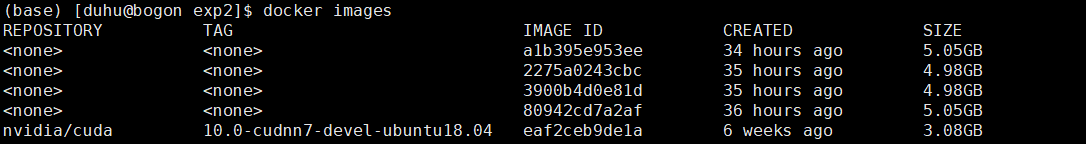
\includegraphics[width=0.9\textwidth]{docker-tag-none}
  \caption{Docker重复安装出现<none>:<none> \label{fig:docker-tag-none}}
\end{figure}

参考\href{https://stackoverflow.com/questions/30179716/what-are-none-repository-and-tags-why-do-they-appear-when-i-use-docker-build}{这里},那在这种情况下,首先我们可以使用指令\textcolor{magenta}{docker rmi \$(docker images -f "dangling=true" -q)}去除掉所有的无效镜像。
然后使用指令\textcolor{magenta}{docker rmi <REPOSITORY>:<TAG>}来删掉所有的镜像,然后重新安装,重新安装的时候,使用指令\textcolor{magenta}{docker build -t <REPOSITORY>:<TAG> -< Dockerfile}。
\chapter{端到端语音识别汇总}
%------------------------------------------------------------------------------
%                                CTC 
%------------------------------------------------------------------------------
\section{CTC}
CTC说实话,就是比较麻烦……我已经看过很多遍了,不过看的原理居多,代码这块,前后向的实现以及梯度的求取这些都没看过……先总结下CTC的基本原理吧还是。

列出本节参考的一些文献和博客:
\begin{enumerate}
  \item CTC的开山之作\upcite{Graves_ctc}\href{http://www.cs.toronto.edu/~graves/icml_2006.pdf}{《Connectionist Temporal Classification: Labelling Unsegmented Sequence Data with Recurrent Neural Networks》},不建议看这篇……因为这篇在讲到求输出序列的时候使用的前后向算法中前向和后向算法的时候对当前时刻$t$的输出概率算了两遍,后面还得再去掉,感觉没啥意思。其次在介绍前后向算法的时候不够简洁,比他的博士论文复杂不少;
  \item Graves大佬的博士毕业论文\upcite{Graves_thesis}\href{https://www.cs.toronto.edu/~graves/preprint.pdf}{《Supervised Sequence Labelling with Recurrent Neural Networks》}里面的推导过程写的就相对来说更清楚一些,过程非常简洁,虽然还有一点点小错误,但是不影响整体的理解,所以推荐看这个来搞清楚CTC的前世今生;
  \item 关于CTC的原理图形化描述请参考\href{https://distill.pub/2017/ctc/}{sequence modeling with ctc\upcite{ctc_graph}},用很多小例子来展现CTC的原理和解码等,有助于去理解结果;
  \item 关于CTC求导部分\upcite{ctc_grad}的得到最后一步结果可以参考\href{https://blog.csdn.net/w5688414/article/details/77867786}{教程:Connectionist Temporal Classification详解补充}。
\end{enumerate}

以上资料看完,我觉得就完全可以理解CTC的原理了,当然手推公式是少不了的,接下来进入正题。
\subsection{白话CTC}
首先明确:语音识别是一个序列分类的任务,那么其输入是逐帧的,如果不知道每一帧对应的标签,那么我们想要用 connectionist network 去干这件事,就得有目标函数。整个神经网络学习的准则就来自于目标函数,所以什么都可以没有,不能没有目标函数;话又说回来了,语音识别在训练的时候,逐帧输入,则必然对应着逐帧的输出,如果不想要对齐,想要端到端,那么就必须想办法把这些逐帧的输出映射成序列输出。真正难的地方就在这儿,怎么去映射,映射了之后怎么定义目标函数;

CTC就是来干这个事情的。

我们先回忆一下使用传统的HMM-DNN模型来搭建语音识别框架,其中包含很多个子任务。首先我们需要使用EM算法训练HMM-GMM模型以拿到对齐的数据,即一帧对应一个音素。其次以这些数据来训练DNN模型,训练好了DNN模型之后,通过HMM和vocabulary映射到更高的建模单元,再结合词典、语言模型来用WFST进行解码。

好的,这个过程很复杂,而且每一块信息量都很足,即要花很多的精力去学习和设计;

不用担心,现在端到端已经越来越火热,效果看上去也是越来越好了。那么咱们说一说CTC是怎么干的。

CTC呢,有一些很重要的设定:\textcolor{red}{(1)每一帧的输出是相互独立的;(2)只要最终映射出来的序列是对的,在任何时刻输出某个标签都可以。}

第一个设定是为了后面使用最大似然估计去定义loss函数的,第二个设定呢就是彻底扔掉对齐数据的限制,按照这个设定,是没有固定的对齐结果的。在讲怎么从连续帧的输出映射到一整个序列之前,我们还要再讲一讲一些规则。为了\textcolor{blue}{避免相邻输出相同和更好的对建模单元的边界进行建模},CTC引入了一个非常重要的输出标签:blank。你可以认为这个东西就是没有标签的意思,因为它的出现对句中无意义的片段比如静音段提供了建模单元。

假设字母表为$A$,则$A^{'}=A\cup\{blank\}$,激活函数的输出$y_k^{t}$为$t$时刻输出$A^{'}$中元素$k$的概率值,给定输入长度为$T$的音频序列$x$;基于输出标签集合$A^{'}$,定义$A^{'^{T}}$为长度为$T$的序列集合。

CTC有如下假设:\textcolor{red}{每一个时间步输出的标签概率值与其他时间步之间相互独立,或者说在$x$的条件下,相互独立}。

那么对于$\pi\in{A^{'^{T}}}$,其条件概率如公式\ref{eqn:ctc-pi}。
\begin{align}
\label{eqn:ctc-pi}
  P(\pi|x) = \prod_{t=1}^{T}y_{\pi_{t}}^{t}
\end{align}

为了和域$A$内的标签序列$l$区分开来,我们称$\pi$为域$A^{'}$内的一条路径。由此定义一个 many-to-one 的函数:$\mathcal{F}:A^{'^{T}}\mapsto{A^{\leq{T}}}$,因为最终系统要输出的是整个正常的序列,而不是穿插着一堆blank还有一堆重复label的奇奇怪怪的东西,我们得到的$\pi$是沿着时间线严格输出的标签值,而$l$是实际上某句话的内容,所以需要$\mathcal{F}$来映射成我们需要的结果,这样才能叫做端到端呀。举个例子,比如某一段音频有15帧,这15帧说的是英文单词"beef",这个就是$l$,那实际上有15帧就会输出15帧的输出结果,可能是这样的"\_ \_ b b \_ e \_ \_ e e \_ f f \_ \_",这个就是$\pi$,$\mathcal{F}$干的事就是把$\pi$映射成$l$,其规则是:
\begin{enumerate}
  \item 合并重复的标签:"\_ \_ b b \_ e \_ \_ e e \_ f f \_ \_" $\longrightarrow$ "\_ b \_ e \_ e \_ f \_";
  \item 移除blank:"\_ b \_ e \_ e \_ f \_" $\longrightarrow$ "beef"。
\end{enumerate}}

这样的路径有很多很多条,而每一条路径都是排他的,因此我们就可以通过公式\ref{eqn:ctc-p}计算出域$A$内某个标签序列的概率值了,即从一段音频中,输出一句话的概率值,CTC牛逼。
\begin{align}
\label{eqn:ctc-p}
  P(l|x) = \sum_{\pi\in{\mathcal{F}^{-1}(l)}}P(\pi|x)
\end{align}

这种整合的意义在于 我不在乎你在什么时间点输出什么,我只在乎最后映射的结果是我想要的。只要最终结果是一样的,中间有多少个blank,同样的标签重复了多少次,我不在乎。这就使得CTC可以使用没有对齐的数据来进行语音识别。

好的,现在还剩下一些问题,公式\ref{eqn:ctc-p}这玩意怎么计算,穷举吗?计算机表示:无能为力。序列越长,标签越多,尤其是碰到汉语这种用字建模的,基本上想都不要想。回想起HMM中讲到的前后向算法,CTC也可以这么干啊,毕竟都是路径概率求解问题。

\subsection{CTC中的前后向算法}
对于公式\ref{eqn:ctc-p},假设标签序列的长度为$U$,音频的长度为$T$,共有$2^{T-U^{2}+U(T-3)}3^{^{(U-1)(T-U)-2}}$条路径。

………………

说实话,我不知道这个是怎么算出来的,但是还是挺恐怖的,还是按照上面举的例子,$U=4$,$T=15$,算一下就是$2^{47}3^{31}$。

………………

再见!

前后向算法的核心是标签序列$l$对应的所有路径概率和可以转换成标签前缀的迭代求和。

为了能让blank出现在输出路径中,我们将$l$修改下,在$l$的前后都加上blank,同时在每个标签之间也都加上blank,记作 $l^{'}$即"b e e f"$\longrightarrow$"\_ b \_ e \_ e \_ f \_"。若$l$的长度为$U$,则$l^{'}$的长度为$U^{'}=2U+1$。为计算$l^{'}$的前缀概率,我们允许blank和non-blank、非重复的non-blank之间直接转换,多解释下这句话的意思:"beef"这个词,"b"在下一个时刻直接跳转到"b"、"e"或者"\_"都是可以的,但是第一个"e"只能跳转到自己本身"e"和"\_",不可以跳转到下一个"e",不然的话,在进行合并操作的时候,第二个"e"就没了,这个需要好好理解,因为后面的前后向算法里面有用到这个特点。

对于一个标签序列$l$,前向变量$\alpha(t,u)$表示所有长度为$t$的路径的概率和,这些路径通过$\mathcal{F}$映射到$l$中长度为$u/2$的前缀,$u/2$向下取整。对于序列$s$,$s_{p:q}$为$s$的子序列${s_p, s_{p+1}, ..., s_{q-1}, s_q}$,定义集合$V(t,u)=\{\pi\in{A^{'^{t}}}:\mathcal{F}(\pi)=l_{1:{u/2}}, \pi_{t}=l_{u}^{'}\}$,则$\alpha(t,u)$的计算如公式\ref{eqn:ctc-forward}。
\begin{align}
\label{eqn:ctc-forward}
  \alpha(t,u) = \sum_{\pi\in{V(t,u)}} \prod_{i=1}^{t}y_{\pi_i}^{i}
\end{align}

我们可以通过$t-1$时刻的前缀来计算$\alpha(t,u)$。

给定上面的公式,我们就可以求得$l$的概率,其等于$T$时刻标签为blank和non-blank的前向概率和,如公式\ref{eqn:ctc-forward-all}。
\begin{align}
\label{eqn:ctc-forward-all}
  p(l|x) = \alpha(T, U^{'}) + \alpha(T, U^{'}-1) 
\end{align}

所有正确的路径一定是以blank或者$l$中的第一个元素开头的,因此我们可以得到$\alpha(t,u)$的初始值,如公式\ref{eqn:ctc-forward-init}。
\begin{align}
\label{eqn:ctc-forward-init}
  \begin{split}
    \alpha(1,1) &= y_{b}^1  \\
    \alpha(1,2) &= y_{l_{1}}^1 \\
    \alpha(1,u) &= 0, \forall u > 2
  \end{split}
\end{align}

初始化的值得到之后,我们可以通过对前缀进行迭代求和的方式得到当前时刻标签索引为$u$的路径概率值,如公式\ref{eqn:ctc-forward-t}。
\begin{align}
\label{eqn:ctc-forward-t}
  \alpha(t,u) = y_{l_{u}^{'}}^{t}\sum_{i=f(u)}^{u} \alpha(t-1,i) 
\end{align}
其中$f(u)$如公式\ref{eqn:ctc-forward-t-start}。
\begin{equation}
\label{eqn:ctc-forward-t-start}
f(u)=\left\{
\begin{array}{rcl}
u-1 & & l_u^{'}=l_{u-2}^{'}\\
u-2 & & otherwise\\
\end{array} \right.
\end{equation}

我觉得有必要解释下公式\ref{eqn:ctc-forward-t-start}。

公式\ref{eqn:ctc-forward-t}左边表示的是在$t$时刻标签索引为$u$的输出概率,右边是在已经确定了$t$时刻输出索引为$u$的情况下,$t-1$时刻的前向概率。因为已经确定了$t$时刻的输出,因此我们需要知道在$t-1$时刻,哪些标签能够在下一个时刻转移到标签$u$。对这些可能的标签前向概率求和,再乘以当前时刻的概率,就得到了我们想要的$\alpha(t,u)$。

那么$t-1$时刻究竟可能是哪些标签呢?

我们还是拿"beef"举例子。

$l=$"b e e f",$l^{'}=$"\_ b \_ e \_ e \_ f \_",为了说的更清楚,我们来给$l^{'}$里面的字母都来标个号,$l^{'}=$"\_(1) b(2) \_(3) e(4) \_(5) e(6) \_(7) f(8) \_(9)"先来看第一种情况,如果$t$时刻的标签$u$有$l_u^{'}=l_{u-2}^{'}$,那么$l_{u}^{'}=$"e(6)"或者$l_{u}^{'}=$"\_(i)",i=\{3,5,7,9\}。
\begin{enumerate}
  \item $l_{u}^{'}=$"e(6)":那么$t-1$时刻的标签等于"e(6)"是完全有可能的;等于\_(5)也是完全可以的;那么能等于e(4)可以吗?假设可以,连起来看$t-1$和$t$时刻的子序列,就是"e(4)e(6)",乍一看好像没问题啊,但是要知道我们在训练的时候"e"是标签,是没有"e(4)"和"e(6)"这种形式的标签的,他们都是"e",根据上面说的CTC的合并规则,这俩就会合并成一个,无法表征两个相同的连续元素。也就是说,CTC是不允许两个相同的连续元素直接跳转过去的,"e(4)"是不可以直接跳转到"e(6)",所以啊,$f(u)=u-1$表示前一个时刻的标签索引只可能和当前时刻的索引相同或者是当前时刻的索引的前一个;
  \item $l_{u}^{'}=$"\_(i)",i=\{3,5,7,9\}:这个解释起来和上面是一样一样的。同样我们的输出标签里面就只有"\_"这个东西,所以按照合并规则,但凡重复了的"\_"都看作是同一个"\_",因此是没有办法表征序列$l^{'}$中的上一个"\_",因此$f(u)=u-1$。
\end{enumerate}

当$l_u^{'} \ne l_{u-2}^{'}$,这个就比较无所谓了,咱们举个例子,假设$l_{u}^{'}=$"f(8)",同样$t-1$时刻的输出为"f(8)"没得问题,"\_(7)"也没得问题,"e(6)"当然也没得问题,反正他们不会乱合并。所以有$f(u)=u-2$。

对应$t$时刻的$u$不能太小,太大无所谓大,大不了剩下的$T-t$帧都重复输出某一个标签或者blank就可以了。如果太小,剩下的$T-t$帧的输出都不够剩下还没有输出的标签了,所以考虑最极端的一种情况就是剩下的每一帧都输出一个$l$中的标签,且这些标签不会自身重复,也就是说每一帧输出的标签都只会输出一次,这样刚好够完整的输出$l$。这就是临界条件,因此我们可以得到$u$的取值范围:
\begin{align}
  T-t \ge \frac{U^{'}-u-1}{2}
\end{align}
解得:
\begin{align}
  u \ge U^{'}-2(T-t) - 1
\end{align}
反过来说,也就是意味着:
\begin{align}
  \alpha(t,u) &= 0, \forall u < U^{'}-2(T-t) - 1
\end{align}

前向算法讲完了,后向算法就很类似了。同样我们定义一个后向变量$\beta(t,u)$,如果说想要得到输出序列$l$,假定$t$时刻的输出是$l_{u}^{'}$,$\beta(t,u)$可以看成是这一些路径的后部分,我们定义$\beta(t,u)$为$t+1$时刻配合上$\alpha(t,u)$恰好构成完整的$l$的所有的后缀路径的概率总和。比照着$V(t,u)$,定义集合$W(t,u)=\{\pi\in{A^{'^{T-t}}:\mathcal{F}(\hat{\pi}+\pi)=l,\forall{\hat{\pi}}\in{V(t,u)}\}$。那么直接计算$\beta(t,u)$的公式如\ref{eqn:ctc-backward}。
\begin{align}
\label{eqn:ctc-backward}
  \beta(t,u) = \sum_{\pi\in{W(t,u)}} \prod_{i=1}^{T-t}y_{\pi_i}^{t+i}
\end{align}

后向算法的初始化如公式\ref{eqn:ctc-backward-init}。
\begin{align}
\label{eqn:ctc-backward-init}
  \begin{split}
    \beta(T,U^{'}) &= 1  \\
    \beta(T,U^{'}-1) &= 1 \\
    \beta(T,u) &= 0, \forall u < U^{'}-1 \\
    \beta(T,U^{'}+1) &= 0
  \end{split}
\end{align}

公式\ref{eqn:ctc-backward-t}描述了$\beta(t,u)$的计算方式。
\begin{align}
\label{eqn:ctc-backward-t}
  \beta(t,u) = \sum_{i=u}^{g(u)} \beta(t+1,i) y_{l_{i}^{'}}^{t+1}
\end{align}
其中:
\begin{equation}
\label{eqn:ctc-backward-t-start}
g(u)=\left\{
\begin{array}{rcl}
u+1 & & l_u^{'}=l_{u+2}^{'}\\
u+2 & & otherwise\\
\end{array} \right.
\end{equation}

公式\ref{eqn:ctc-backward-t-start}表明了对$t+1$时刻能达到的标签的限制,这部分和前向很类似,在此就不再赘述了。

同样后向算法中的$u$不能太大,因为$u$过大的意思就是前$t$个时刻得输出$u$个标签,如果说$t$稍微小了点,那就不够输出这么多标签了。同样,考虑临界条件:前$t$个时刻恰好能够无重复的输出non-blank标签。我们就可以得到如下不等式:
\begin{align}
  t \ge \frac{u}{2}
\end{align}
解得:
\begin{align}
  u \leq 2t
\end{align}
即:
\begin{align}
  \beta(t,u) &= 0, \forall u > 2t
\end{align}

到这儿,CTC中的前后向算法就讲完了,下一步是定义loss函数和求梯度。

\subsection{CTC中的loss函数和梯度}
对于数据集$\mathcal{S}$,CTC的损失函数$\mathcal{L}(\mathcal{S})$定义为数据集中所有输出序列正确的负$\log$概率,如公式\ref{eqn:ctc-loss}。
\begin{align}
\label{eqn:ctc-loss}
  \begin{split}
    \mathcal{L}(\mathcal{S}) &= -\ln{\prod_{(x,z)\in{S}}}p(z|x) \\
                             &= -\sum_{(x,z)\in{S}}\ln p(z|x)
  \end{split}
\end{align}

因为损失函数是可微分的,所以我们可以通过BPTT(以后这块也得写个总结)去求权重对的梯度。所以任何一个基于梯度的非线性优化函数都可用来训练CTC网络。我们先看下单个样本的loss,如公式\ref{eqn:ctc-loss-one}。
\begin{align}
\label{eqn:ctc-loss-one}
  \mathcal{L}(x,z) = -\ln p(z|x)
\end{align}
则有:
\begin{align}
 \mathcal{L}(\mathcal{S}) = \sum_{(x,z)\in{S}}\mathcal{L}(x,z)
\end{align}
从而有:
\begin{align}
 \frac{\partial{\mathcal{L}(\mathcal{S})}}{\partial{w}} = \sum_{(x,z)\in{S}} \frac{\partial{\mathcal{L}(x,z)}}{\partial{w}}
\end{align}

设$l=z$,定义集合$X(t,u)=\{\pi\in{A^{'^{T}}}:\mathcal{F}(\pi)=z, \pi_{t}=z_{u}^{'}\}$,这个$X(t,u)$表示的是所有最终整合之后的序列为$z$,且在$t$时刻输出索引为$u$的路径集合。根据公式\ref{eqn:ctc-forward}和公式\ref{eqn:ctc-backward},我们可以得到在集合$X(t,u)$中的所有路径元素的概率和,如公式\ref{eqn:ctc-forback}。
\begin{align}
\label{eqn:ctc-forback}
  \alpha(t,u)\beta(t,u) = \sum_{\pi\in{X(t,u)}}\prod_{t=1}^{T} y_{\pi_{t}}^{t}
\end{align}

公式\ref{eqn:ctc-forback}中说明了当$t$时刻,输出的标签索引为$u$的所有路径的可能性,那么我们希望获得的是输出$z$的概率值,那么我们只需要知道$t$时刻共有多少个可能的标签,然后对这些标签按照公式\ref{eqn:ctc-forback}去求解,最后将这些可能性都加起来,不就得到了输出序列$z$的概率值了吗?

所以我们得到了输出序列$z$的概率值如公式\ref{eqn:ctc-ouput-prob}。
\begin{align}
\label{eqn:ctc-ouput-prob}
  p(z|x) = \sum_{u=1}^{|z^{'}|}\alpha(t,u)\beta(t,u)
\end{align}

那么单个样本的损失函数我们就可以算出来了,如公式\ref{eqn:ctc-loss-var}。
\begin{align}
\label{eqn:ctc-loss-var}
 \mathcal{L}(x,z) &= -\ln \sum_{u=1}^{|z^{'}|}\alpha(t,u)\beta(t,u)
\end{align}

\subsection{CTC的解码}
CTC的解码常用的有两种方式,greedy search和prefix beam search。greedy解码速度很快,但是很容易出错,但是prefix beam search解码速度慢,准确率较高。接下来挨个介绍两种解码方式的算法和流程,以及对应的代码解释。

\subsubsection{greedy search}


\subsubsection{prefix beam search}
First-Pass Large Vocabulary Continuous Speech Recognition using Bi-Directional Recurrent DNNs\upcite{prefix-bs}中针对CTC提出了一种prefix beam search的算法,这种算法能够避免全局搜索的复杂度过高无法实现的问题,同时比greedy search的结果要好很多。

首先介绍下一些公式。公式\ref{eqn:with-lm}是最终的解码公式,配合语言模型和网络输出(声学模型),得到最有可能的$W$词序列。
\begin{align}
\label{eqn:with-lm}
W = \arg\mathop{\max}_{W}p_{net}(W;X)p_{lm}^{\alpha}(W)|W|^{\beta}
\end{align}
其中$p_{net}$是网络的输出,$p_{lm}$是语言模型的输出,$\alpha$和$\beta$分别为语言模型的权重和补偿系数。一般情况下,我们会降低语言模型对整体输出的影响,所以$\alpha$一般取$0.2$ \~ $0.7$。

接下来我们讲一下prefix beam search的demo\upcite{prefix-beam-search}。

总体是有三个循环,第一个是时间维度上的,时间$t$从$1$到$T$,也就是逐帧解码。第二个是对应候选输出序列的,这个是beam search,那么一定得设置一个beam size,那么会考虑所有的候选序列跟当前输出结合起来的概率值,那当前输出的话被剪枝之后还有很多个标签,再挨个的把每一个候选和每一个当前帧的标签进行结合计算。然后再利用这个结合的概率值进行重新排序得到新的候选。

\begin{lstlisting}[language = shell, numbers=left, 
         numberstyle=\tiny,keywordstyle=\color{blue!70},
         commentstyle=\color{red!50!green!50!blue!50},frame=shadowbox,
         rulesepcolor=\color{red!20!green!20!blue!20},basicstyle=\ttfamily]
pruned_alphabet = [alphabet[i] for i in np.where(ctc[t] > prune)[0]]
\end{lstlisting}

这一步是为了减少计算,也就是说先设定一个阈值,当前$t$时刻的时候,会做一个判断,只有当前时刻各个标签概率值大于 prune 的时候才会去做后续的操作,这就意味着当前时刻所有概率低于 prune 的标签都会被抛弃,不再参与到当前时刻的解码过程中。因为这些标签概率值太小,不太可能是正确的输出标签,留着只会增加计算量,还不如删掉,省时省心省力!

\begin{lstlisting}[language = shell, numbers=left, 
         numberstyle=\tiny,keywordstyle=\color{blue!70},
         commentstyle=\color{red!50!green!50!blue!50},frame=shadowbox,
         rulesepcolor=\color{red!20!green!20!blue!20},basicstyle=\ttfamily]
if len(l) > 0 and l[-1] == '>':
  Pb[t][l] = Pb[t - 1][l]
  Pnb[t][l] = Pnb[t - 1][l]
  continue 
\end{lstlisting}

这一步就是判断下是不是到结尾了,结尾的表示符号是">"。如果到了结尾呢,说明这个时候输出的标签序列和$t-1$时刻是一毛一样滴。$t$时刻输出序列$l$以 blank 结尾的概率跟$t-1$时刻以 blank 结尾的概率是一样的,$t$时刻输出序列$l$以 non-blank 结尾的概率跟$t-1$时刻以 non-blank 结尾的概率是一样的。然后就跳出当前时刻,因为当前时刻表示这个序列已经到了结尾了,没必要再折腾下去了。
 
\begin{lstlisting}[language = shell, numbers=left, 
         numberstyle=\tiny,keywordstyle=\color{blue!70},
         commentstyle=\color{red!50!green!50!blue!50},frame=shadowbox,
         rulesepcolor=\color{red!20!green!20!blue!20},basicstyle=\ttfamily]
if c == '%':
  Pb[t][l] += ctc[t][-1] * (Pb[t - 1][l] + Pnb[t - 1][l])
\end{lstlisting}

我们假设$\%$代表blank这个标签。剪枝之后,会对还剩下的那些标签走一遍遍历,每一个标签都会尝试着和之前存起来的候选序列进行结合,算出来一个概率值。那么既然是遍历,当然会轮到牛逼的 blank。所以首先看看当前的这个标签是不是blank。如果是blank的话,我们就没必要对当前的这个候选序列做啥子改动了,也就是当前时刻的输出标签序列还是$l$,因为最终输出的时候,blank也不会出现。既然当前这个标签是blank,那么$t$时刻的标签序列$l$的概率需要和当前时刻输出为 blank 的概率结合一下,变成当前时刻的 $Pb[t][l]$。其计算公式从代码里就可以看到。

\begin{lstlisting}[language = shell, numbers=left, 
         numberstyle=\tiny,keywordstyle=\color{blue!70},
         commentstyle=\color{red!50!green!50!blue!50},frame=shadowbox,
         rulesepcolor=\color{red!20!green!20!blue!20},basicstyle=\ttfamily]
l_plus = l + c
if len(l) > 0 and c == l[-1]:
  Pnb[t][l_plus] += ctc[t][c_ix] * Pb[t - 1][l]
  Pnb[t][l] += ctc[t][c_ix] * Pnb[t - 1][l]
\end{lstlisting}

如果说当前时刻的标签不是 blank,而是上个时刻的这个候选序列的最后一个输出标签,也就是说当前时刻的输出和上一个时刻的候选序列尾部产生了重复,这个时候其实是有两种情况的,第一种情况是上一个时刻的输出标签正好是 blank,因为从上面那一步代码中我们可以看出来,候选序列中是不会出现blank的,那如果是这种的情况,说明实际的输出序列就是有两个一样的字母,输出就是$l\_plus$,其尾部有两个一样的字母,这个时候候选序列的概率就等于当前时刻的标签概率乘以上一个时刻输出为blank的序列概率,也就是$Pb[t - 1][l]$;第二种情况是上一个时刻的输出确实也是这个标签,那么说明这个时候的候选序列不需要做啥变动,但是概率值需要变一下,当前时刻标签概率乘以上一个时刻输出是 non-blank 的序列概率值。

\begin{figure}[h]
  \centering
  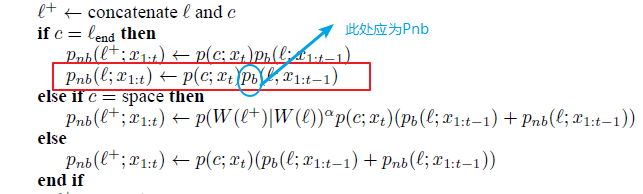
\includegraphics[width=0.6\textwidth]{error-prefix}
  \caption{Prefix Beam Search原论文中算法错误地方 \label{fig:error-prefix}}
\end{figure}

另外原论文中关于这一块的计算步骤写错了,也就是算法中的这一步,如图\ref{fig:error-prefix}。简直坑死个人。

\begin{lstlisting}[language = shell, numbers=left, 
         numberstyle=\tiny,keywordstyle=\color{blue!70},
         commentstyle=\color{red!50!green!50!blue!50},frame=shadowbox,
         rulesepcolor=\color{red!20!green!20!blue!20},basicstyle=\ttfamily]
elif len(l.replace(' ', '')) > 0 and c in (' ', '>'):
  lm_prob = lm(l_plus.strip(' >')) ** alpha
  Pnb[t][l_plus] += lm_prob * ctc[t][c_ix] * (Pb[t - 1][l] + Pnb[t - 1][l])
\end{lstlisting}

那还有可能当前的输出是 ' '(space),也就是说输出是空格或者是结尾,这个时候说明一个完整的词出现了,我们就可以利用语言模型(LM)来对输出进行修正和约束,避免出现毫无意义的结果。那么这个词代入到语言模型中会出现一个概率值,当前候选序列的概率值就通过公式\ref{eqn:with-lm}来计算,从代码中也可以看出来。

\begin{lstlisting}[language = shell, numbers=left, 
         numberstyle=\tiny,keywordstyle=\color{blue!70},
         commentstyle=\color{red!50!green!50!blue!50},frame=shadowbox,
         rulesepcolor=\color{red!20!green!20!blue!20},basicstyle=\ttfamily]
Pnb[t][l_plus] += ctc[t][c_ix] * (Pb[t - 1][l] + Pnb[t - 1][l])
\end{lstlisting}

还有最后一种情况,就是既不是 blank,又不是 space,当前输出标签和候选标签序列的最后一个字母也不一样,这个时候,就直接算出候选标签序列和当前标签的概率乘积就行,候选标签序列也有两种情况:上一个时刻以blank或者以non-blank结尾。综上集中基本的情况都已经讲完了。

\begin{lstlisting}[language = shell, numbers=left, 
         numberstyle=\tiny,keywordstyle=\color{blue!70},
         commentstyle=\color{red!50!green!50!blue!50},frame=shadowbox,
         rulesepcolor=\color{red!20!green!20!blue!20},basicstyle=\ttfamily]
if l_plus not in A_prev:
  Pb[t][l_plus] += ctc[t][-1] * (Pb[t - 1][l_plus] + Pnb[t - 1][l_plus])
  Pnb[t][l_plus] += ctc[t][c_ix] * Pnb[t - 1][l_plus]
\end{lstlisting}

按照原始论文中,还有上面这个公式。也就是说算出来的$l\_plus$不在候选标签序列里面,就会去之前时刻的候选序列里面去找,再利用之前的后续序列概率计算当前的概率值。百度的Deep Speech2代码里面说:这个部分不知道在干啥,还没啥用,所以就给去掉了。

我觉得……也不太好理解……

讲到这儿核心的代码部分已经讲完了,剩下的就是把当前时刻的标签,不管是以blank结尾的还是非blank结尾的综合起来,然后进行排序,根据beam size的大小得到新的候选序列,如此循环往复,直到这个序列输出到了尽头,就可以得到最终的结果啦\~\~\~

完整代码如下:

%%%%%%%%%%%%%%%%%%%%%%%Code for Prefix Beam Search%%%%%%%%%%%%%%%%%%%%%%%%%%%%%%%%%
\begin{lstlisting}[language = python, numbers=left, 
         numberstyle=\tiny,keywordstyle=\color{blue!70},
         commentstyle=\color{red!50!green!50!blue!50},frame=shadowbox,
         rulesepcolor=\color{red!20!green!20!blue!20},basicstyle=\ttfamily]
from collections import defaultdict, Counter
from string import ascii_lowercase
import re
import numpy as np

def prefix_beam_search(ctc, lm=None, k=25, alpha=0.30, beta=5, prune=0.001):
  """
  Performs prefix beam search on the output of a CTC network.

  Args:
    ctc (np.ndarray): The CTC output. Should be a 2D array (timesteps x alphabet_size)
    lm (func): Language model function. Should take as input a string and output a probability.
    k (int): The beam width. Will keep the 'k' most likely candidates at each timestep.
    alpha (float): The language model weight. Should usually be between 0 and 1.
    beta (float): The language model compensation term. The higher the 'alpha', the higher the 'beta'.
    prune (float): Only extend prefixes with chars with an emission probability higher than 'prune'.

  Retruns:
    string: The decoded CTC output.
  """

  lm = (lambda l: 1) if lm is None else lm # if no LM is provided, just set to function returning 1
  W = lambda l: re.findall(r'\w+[\s|>]', l)
  alphabet = list(ascii_lowercase) + [' ', '>', '%']
  F = ctc.shape[1]
  ctc = np.vstack((np.zeros(F), ctc)) # just add an imaginative zero'th step (will make indexing more intuitive)
  T = ctc.shape[0]

  # STEP 1: Initiliazation
  O = ''
  Pb, Pnb = defaultdict(Counter), defaultdict(Counter)
  Pb[0][O] = 1
  Pnb[0][O] = 0
  A_prev = [O]
  # END: STEP 1

  # STEP 2: Iterations and pruning
  for t in range(1, T):
    pruned_alphabet = [alphabet[i] for i in np.where(ctc[t] > prune)[0]]
    for l in A_prev:
      
      if len(l) > 0 and l[-1] == '>':
        Pb[t][l] = Pb[t - 1][l]
        Pnb[t][l] = Pnb[t - 1][l]
        continue  

      for c in pruned_alphabet:
        c_ix = alphabet.index(c)
        # END: STEP 2
        
        # STEP 3: “Extending” with a blank
        if c == '%':
          Pb[t][l] += ctc[t][-1] * (Pb[t - 1][l] + Pnb[t - 1][l])
        # END: STEP 3
        
        # STEP 4: Extending with the end character
        else:
          l_plus = l + c
          if len(l) > 0 and c == l[-1]:
            Pnb[t][l_plus] += ctc[t][c_ix] * Pb[t - 1][l]
            Pnb[t][l] += ctc[t][c_ix] * Pnb[t - 1][l]
        # END: STEP 4

          # STEP 5: Extending with any other non-blank character and LM constraints
          elif len(l.replace(' ', '')) > 0 and c in (' ', '>'):
            lm_prob = lm(l_plus.strip(' >')) ** alpha
            Pnb[t][l_plus] += lm_prob * ctc[t][c_ix] * (Pb[t - 1][l] + Pnb[t - 1][l])
          else:
            Pnb[t][l_plus] += ctc[t][c_ix] * (Pb[t - 1][l] + Pnb[t - 1][l])
          # END: STEP 5

          # STEP 6: Make use of discarded prefixes
          if l_plus not in A_prev:
            Pb[t][l_plus] += ctc[t][-1] * (Pb[t - 1][l_plus] + Pnb[t - 1][l_plus])
            Pnb[t][l_plus] += ctc[t][c_ix] * Pnb[t - 1][l_plus]
          # END: STEP 6

    # STEP 7: Select most probable prefixes
    A_next = Pb[t] + Pnb[t]
    sorter = lambda l: A_next[l] * (len(W(l)) + 1) ** beta
    A_prev = sorted(A_next, key=sorter, reverse=True)[:k]
    # END: STEP 7

  return A_prev[0].strip('>')

\end{lstlisting}

%------------------------------------------------------------------------------
%                                RNN Tranducer 
%------------------------------------------------------------------------------
\section{RNN-Tranducer}

%------------------------------------------------------------------------------
%                                Attention 
%------------------------------------------------------------------------------
\section{Attention}

%------------------------------------------------------------------------------
%                                Transformer 
%------------------------------------------------------------------------------
\section{Transformer}


%------------------------------------------------------------------------------
%                                CNNs 
%------------------------------------------------------------------------------
\section{CNNs}

%------------------------------------------------------------------------------
%                                Mixed Models 
%------------------------------------------------------------------------------
\section{Mixed Models}

\subsection{Self-Attention Transducers for End-to-End Speech Recognition}
这篇论文的作者是田正坤,来自中国科学院自动化所。本论文的主要贡献有:
\begin{enumerate}
  \item 用self-attention模块替代了原来RNN-T中的RNN部分,可以用于并行计算;
  \item 利用 path-aware regularization 帮助SA-T学习对齐;
  \item 使用了chunk-flow机制来进行解码。
\end{enumerate}

\subsubsection{SA-T的基本结构}

\subsubsection{path-aware regularization}

\subsubsection{chunk flow mechanism}


\chapter{论文阅读笔记}

\section{Light Gated Recurrent Units for Speech Recogntion}

\href{https://arxiv.org/abs/1803.10225}{Li-GRU}是Mirco Ravanelli于2018年发表的论文,他也是\href{https://arxiv.org/abs/1811.07453}{pytorch-kaldi}的作者。这篇论文主要针对的是对\href{https://arxiv.org/abs/1406.1078}{GRU}(Gated Recurrent Units)的改进,而且Li-GRU是专门为语音识别去设计的。本论文主要的工作有两方面:

(1)去掉了重置门(reset gate),去掉重置门对于模型的效果没什么影响,而且原始的GRU的重置门和更新门之间有冗余,因此去掉重置门的模型结构更合理;
  
(2)将原始GRU中的激活函数Tanh换成了Relu,由于Relu本身函数具备的特性,其效果比Relu要好多。之所以以前的RNN(包括GRU和LSTM)不用Relu,是因为Relu的值可以任意大,RNN不停的迭代中,Relu的值无法控制,容易导致数值不稳定(numerical instability)。本文作者采用了批量正则(Batch Normalization)的方式来避免数值不稳定的情况。这么做既可以避免梯度消失,又可以加速网络收敛,减少网络的时间。


本节的论文笔记分为三个部分:(1)GRU的介绍;(2)Li-GRU的学习;(3)实验配置和结果;(4)个人心得体会。

\subsection{GRU的介绍}
\label{sub:gru}
语音识别是一个序列任务,那么上下文的信息对当前时刻信息的影响很大,RNN的结构表明其可以动态的决定对于当前时间步使用多少上下文的信息。但是RNN存在的梯度消失和爆炸问题使得其学习长期依赖变得困难。所以一般我们都会使用一种门控RNN(Gated RNN)来解决这个问题。门控RNN的核心思想是引入一种门机制来控制不同时间步之间的信息流动。

常用的门控RNN有两种:LSTM和GRU。LSTM的结构复杂且运算效率比较低,LSTM有三个门,而GRU只有两个,所以运算起来快很多。而本论文也是基于GRU做的改进,所以不讨论LSTM。

GRU的计算公式如下:
\begin{align}
z_t &= \sigma(W_{z}x_{t}+U_{z}h_{t-1}+b_z) \label{eqn:up-gate} \\
r_t &= \sigma(W_{r}x_{t}+U_{r}h_{t-1}+b_r) \label{eqn:re-gate} \\
\tilde{h}_{t} &= tanh(W_{h}x_{t}+U_{h}(h_{t-1}\odot{r_{t}})+b_{h}) \label{eqn:candi-h} \\
h_{t} &= z_{t}\odot{h_{t-1}} + (1-z_{t})\odot\tidle{h}_{t}  \label{eqn:final-h}
\end{align}
其中
\begin{itemize}
  \item \textit{$x_t$:t时刻输入特征向量} 
  \item \textit{$r_t$:t时刻重置门向量}  
  \item \textit{$u_t$:t时刻更新门向量}
  \item \textit{$h_t$:t时刻状态向量}
  \item \textit{$\tidle{h}_t$:t时刻候选状态向量}
  \item \textit{$W,U,b$:参数矩阵和向量}

\end{itemize}\\


由公式\ref{eqn:final-h}可知,当前状态向量$h_t$是前一刻状态向量$h_{t-1}$和当前时刻的状态候选向量$\tilde{h}_{t}$之间的一个\href{https://zh.wikipedia.org/zh-hans/\%E7\%BA\%BF\%E6\%80\%A7\%E6\%8F\%92\%E5\%80\%BC}{线性插值}。两者之间的权重由更新门$z_{t}$决定,权重的值表示了更新信息的多少。这个线性插值就是GRU学习长期依赖的核心。如果$z_{t}$接近于$1$,那么先前状态的信息就得以保留,以此学习到间隔长的时间步之间的信息关联。如果$z_t$接近于$0$,那么网络更倾向于候选状态$\tilde{h}_{t}$,而候选状态更依赖于当前输入和临近时间步的状态。同时候选状态还依赖于重置门$r_{t}$,其使得模型通过忘记之前计算的状态来清除过去的记忆。

GRU的模型结构图如\ref{fig:gru}所示。
\begin{figure}[htbp]
  \centering
  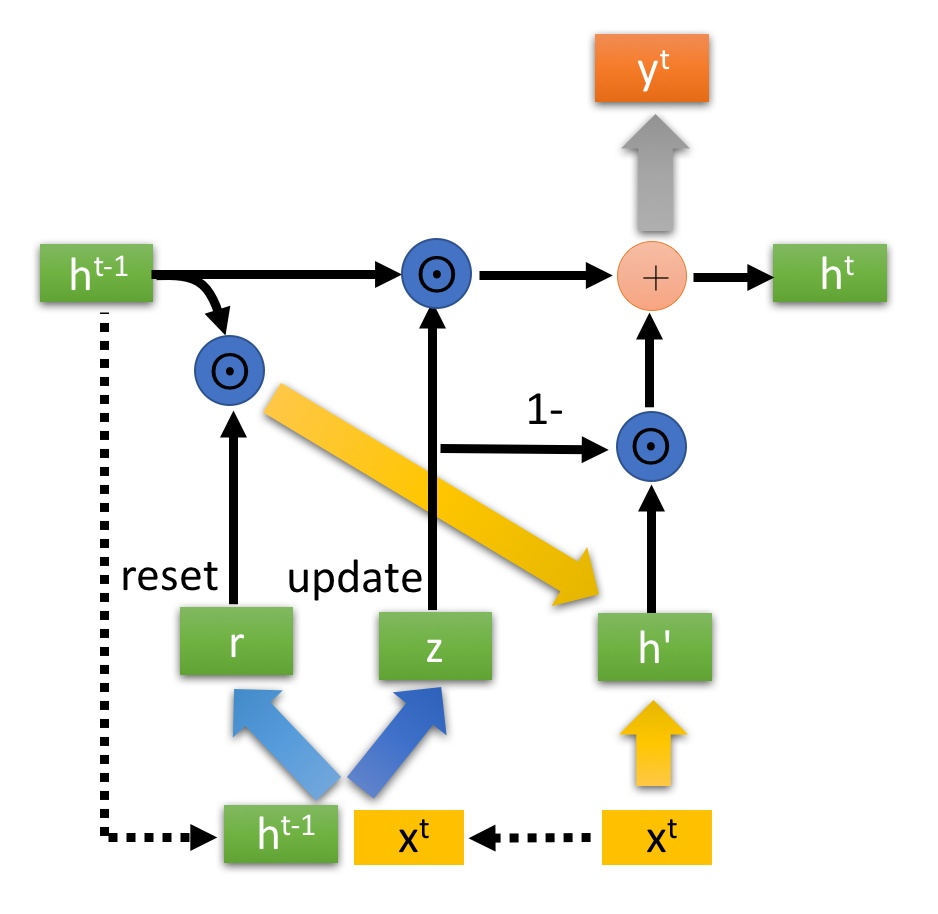
\includegraphics[width=0.45\textwidth]{gru-architecture}
  \caption{GRU模型结构图 \label{fig:gru}}
\end{figure}

\subsection{Li-GRU的学习}
\label{sec:li-gru}
本论文对GRU的改进主要涉及到三个部分:重置门、ReLU激活函数和BN。

1.移除重置门:

对于序列中可能出现的 significant discontinuity,重置门可以起到一个清除过去信息的作用。比如说语言建模,当输入从一个句子跳转到另一个语义无关的句子的时候,重置门就可以起到很好的作用:避免过去无关信息对当前状态的干扰。但是对于语音识别来说,重置门的作用可能就不明显了,语音识别中的输入变化都比较小(一般的偏移量才10ms),这表明过去的信息还是挺有用的。即便是元音(Vowel)和擦音(Fricative)间的边界有很强的不连续现象,完全去掉过去信息也可能是有害的。另外基于一些音素的转移更相似,存住 phonotactic features 还是很有用的。

与此同时,重置门和更新门之间存在着某种冗余。也就是说$z_t$和$r_t$的变化比较同步,当前输入信息比较重要的时候,$z_t$和$r_t$都比较小;过去时刻信息比较重要的时候,$z_t$和$r_t$都比较大。拿TIMIT中的一段音频来看,更新门和重置门的平均激活值有着时域上的关联性,如图\ref{fig:ru-correlation}。
\begin{figure}[htbp]
  \centering
  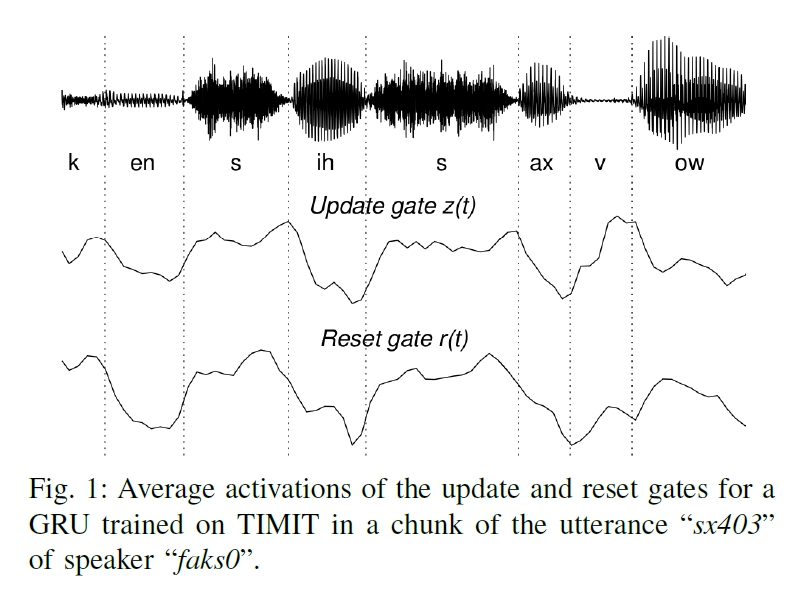
\includegraphics[width=0.45\textwidth]{rucor}
  \caption{TIMIT中更新门与重置门音频上的时域关联 \label{fig:ru-correlation}}
\end{figure}

两个门之间的冗余程度可以量化描述,其公式 cross-correlation $C(z,r)$如下:
\begin{align}
\label{eqn:rucor}
C(z,r) = \bar{z}_t \star \bar{r}_t
\end{align}
其中:
\begin{itemize}
  \item \textit{$\bar{z}_t$:更新门神经元的平均激活值}
  \item \textit{$\bar{r}_t$:重置门神经元的平均激活值}
  \item \textit{$\star$:cross-correlation 的算子} 
\end{itemize}

图\ref{fig:aver-cor}显示了重置门和更新门的 cross-correlation。门激活值计算的是所有的输入帧,所有的隐藏神经元的激活值计算了个平均。从图中我们可以看到重置门和更新门之间相似度还挺高,因此冗余程度也很高。
\begin{figure}[htbp]
  \centering
  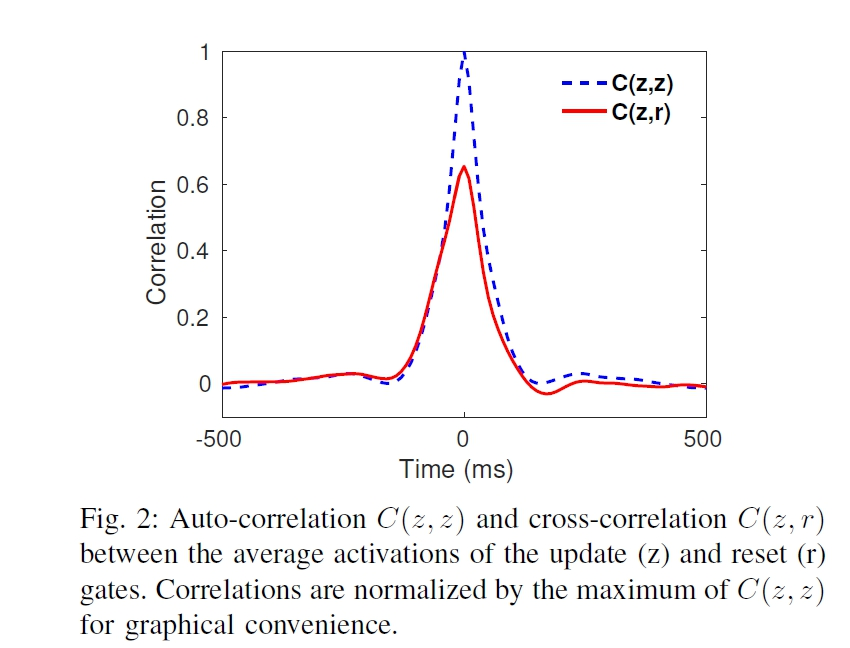
\includegraphics[width=0.45\textwidth]{aver-cor}
  \caption{Auto-correlation $C(z,z)$和cross-correlation $C(z,r)$ \label{fig:aver-cor}}
\end{figure}

因此我们决定去掉重置门,那么公式\ref{eqn:candi-h}就变成了公式\ref{eqn:candi-h-no-reset}。这么处理之后,运算效率就提高了,就剩下一个门,所以GRU的结构变得更紧凑了。
\begin{align}
\label{eqn:candi-h-no-reset}
\tilde{h}_{t} &= tanh(W_{h}x_{t}+U_{h}h_{t-1}+b_{h})
\end{align}

2. ReLU激活函数

我们将tanh替换成ReLU。tanh其实在前馈神经网络中很少使用,因为当神经网络的层数变深时,它就容易陷入左右的边界值$-1$和$1$,此时的梯度接近于$0$,网络参数更新缓慢,收敛的也就很慢。ReLU就不存在这样的问题,但是ReLu的值域没有边界,因此容易出现一些数值问题,为了解决这个问题,我们将ReLU和BN一起使用,这样就很不存在数值问题了。将tanh改为ReLU之后,GRU的公式如下:
\begin{align}
\label{eqn:candi-h-no-reset-relu}
\tilde{h}_{t} &= ReLU(W_{h}x_{t}+U_{h}h_{t-1}+b_{h})
\end{align}

3.BN

神经网络训练时,计算每一个 mini-batch 每层激活前输出的均值和方差,再利用均值和方差对激活前输出进行归一化能够解决所谓的 internal covariate shift 问题,这个就是传说中的Batch Normalization。BN既可以加快网络训练速度,又可以提高模型的效果。本文中只对前馈部分进行BN操作,因为其只对前馈神经网络进行操作,完全可以实现并行计算。其公式如下:
\begin{align}
z_t &= \sigma(BN(W_{z}x_{t})+U_{z}h_{t-1}) \label{eqn:bn-up-gate} \\
\tilde{h}_{t} &= ReLU(BN(W_{h}x_{t})+U_{h}h_{t-1}) \label{bn-eqn:candi-h} \\
h_{t} &= z_{t}\odot{h_{t-1}} + (1-z_{t})\odot\tidle{h}_{t}  \label{eqn:bn-final-h}
\end{align}
其中$BN(\cdot)$如公式\ref{eqn:bn}所示,$\mu_{b}$和$\sigma_{b}$分别为当前mini-batch的均值和方差。
\begin{align}
\label{eqn:bn}
BN(a) = \gamma \odot \frac{a-\mu_{b}}{\sqrt{(\sigma_b)^{2}+\epsilon}} + \beta
\end{align}

因为BN中已经包含了$\beta$,因此之前公式中的偏置$b_z$和$b_h$就不再需要了。Li-GRU将ReLU和BN结合起来,既利用了ReLU和BN两者的优点,同时还避免了ReLU的数值不稳定问题。

\subsection{个人心得体会}
\label{sec:ligru-pers}
综上所言,Li-GRU通过减少了一个重置门来达到轻量级的效果,与此同时根据语音识别任务的特殊性,其认为语音序列任务中,对过往记忆清零对模型效果是有伤害的,而且重置门和更新门之间关联比较深,两个门显得冗余,因此其去掉了重置门。为了让网络更新更快,效果更好,以Relu函数代替了tanh作为候选状态的激活函数,同时以BN来解决Relu无边界的数值问题。BN还可以帮助快速训练和提升效果。

附上一些音素的分类,如表\ref{tab:phone-category}
\begin{table}[htbp]
   \centering
   \caption{音素分类及示例}
     \begin{tabular*}{1\textwidth}{@{\extracolsep{\fill}}ccc}
     \toprule
     Phonetic Cat. &音素类别       & Phone Lists \\
     \midrule
     Vowels        &元音          & \{iy, ih, eh, ae, ..., oy, aw, ow, er\}  \\
     Liquids       &流音          & \{l, r, y, w, el\}  \\
     Nasals        &鼻音          & \{en, m, n, ng\}  \\
     Fricatives    &擦音          & \{ch, jh, dh, z, v, f, th, s, sh, hh, ,zh\}   \\
     Stops         &塞音          & \{b, d, g, p, t, k, dx, cl, vcl, epi\}   \\
     \bottomrule
     \end{tabular}%
   \label{tab:phone-category}%
 \end{table}%


\chapter{深度学习框架笔记}
\section{paddlepaddle}
本处记录一些用paddlepaddle跑百度的DeepSpeech2的笔记和问题:
\begin{enumerate}
	\item 基于一些原因,服务器A上的GPU暂时不可用,因此在服务器B上重新部署了百度基于paddlepaddle的\href{https://github.com/PaddlePaddle/DeepSpeech}{DS2}。A和B有共享目录,因此这个repository是放在一个共享目录下的,但是在运行./run_\train.sh之后,模型初始化没有任何问题,log显示已经开始在训练了,但是在存模型那块死活不动。因为之前在服务器A上训练过一段时间,所以对应存储checkpoint的路径是服务器A的用户创建的,如果没有给够权限的话,服务器B是没有办法存储checkpoint到原来服务器A的那个文件夹下的,所以两种办法:给够路径足够的权限或者以服务器B的用户重新创建一个路径;
	\item 在利用训练和测试数据生成vocab.txt的时候,因为是从对应的文本中提取的vocab.txt,不同的数据库文本不一样,所以最终生成的vocab.txt也是不一样的。千万不要用其他数据库的vocab.txt来对当前库进行训练或者测试,因为结果会惨不忍睹;
	\item DS2提取的音频特征是80维的fbank。
\end{enumerate}}

\section{pytorch}

\section{tensorflow}


%\bibliography{reference/chap1,reference/chap2} %多个章节的参考文献
\bibliography{references/asr-references}

%%%%%%%%%%%%%%%%%%%%%%%%%%%%%%
%% 后置部分
%%%%%%%%%%%%%%%%%%%%%%%%%%%%%%

%% 附录(章节编号重新计算,使用字母进行编号)
%\appendix
%\renewcommand\theequation{\Alph{chapter}--\arabic{equation}}  % 附录中编号形式是"A-1"的样子
%\renewcommand\thefigure{\Alph{chapter}--\arabic{figure}}
%\renewcommand\thetable{\Alph{chapter}--\arabic{table}}

%\include{chapters/app1} 
%\include{chapters/app2} 


\end{document}
